% Options for packages loaded elsewhere
\PassOptionsToPackage{unicode}{hyperref}
\PassOptionsToPackage{hyphens}{url}
%
\documentclass[
]{article}
\usepackage{amsmath,amssymb}
\usepackage{lmodern}
\usepackage{ifxetex,ifluatex}
\ifnum 0\ifxetex 1\fi\ifluatex 1\fi=0 % if pdftex
  \usepackage[T1]{fontenc}
  \usepackage[utf8]{inputenc}
  \usepackage{textcomp} % provide euro and other symbols
\else % if luatex or xetex
  \usepackage{unicode-math}
  \defaultfontfeatures{Scale=MatchLowercase}
  \defaultfontfeatures[\rmfamily]{Ligatures=TeX,Scale=1}
\fi
% Use upquote if available, for straight quotes in verbatim environments
\IfFileExists{upquote.sty}{\usepackage{upquote}}{}
\IfFileExists{microtype.sty}{% use microtype if available
  \usepackage[]{microtype}
  \UseMicrotypeSet[protrusion]{basicmath} % disable protrusion for tt fonts
}{}
\makeatletter
\@ifundefined{KOMAClassName}{% if non-KOMA class
  \IfFileExists{parskip.sty}{%
    \usepackage{parskip}
  }{% else
    \setlength{\parindent}{0pt}
    \setlength{\parskip}{6pt plus 2pt minus 1pt}}
}{% if KOMA class
  \KOMAoptions{parskip=half}}
\makeatother
\usepackage{xcolor}
\IfFileExists{xurl.sty}{\usepackage{xurl}}{} % add URL line breaks if available
\IfFileExists{bookmark.sty}{\usepackage{bookmark}}{\usepackage{hyperref}}
\hypersetup{
  pdftitle={Using generalized additive models to analyze biomedical non-linear longitudinal data},
  hidelinks,
  pdfcreator={LaTeX via pandoc}}
\urlstyle{same} % disable monospaced font for URLs
\usepackage[margin=1in]{geometry}
\usepackage{listings}
\newcommand{\passthrough}[1]{#1}
\lstset{defaultdialect=[5.3]Lua}
\lstset{defaultdialect=[x86masm]Assembler}
\usepackage{longtable,booktabs,array}
\usepackage{calc} % for calculating minipage widths
% Correct order of tables after \paragraph or \subparagraph
\usepackage{etoolbox}
\makeatletter
\patchcmd\longtable{\par}{\if@noskipsec\mbox{}\fi\par}{}{}
\makeatother
% Allow footnotes in longtable head/foot
\IfFileExists{footnotehyper.sty}{\usepackage{footnotehyper}}{\usepackage{footnote}}
\makesavenoteenv{longtable}
\usepackage{graphicx}
\makeatletter
\def\maxwidth{\ifdim\Gin@nat@width>\linewidth\linewidth\else\Gin@nat@width\fi}
\def\maxheight{\ifdim\Gin@nat@height>\textheight\textheight\else\Gin@nat@height\fi}
\makeatother
% Scale images if necessary, so that they will not overflow the page
% margins by default, and it is still possible to overwrite the defaults
% using explicit options in \includegraphics[width, height, ...]{}
\setkeys{Gin}{width=\maxwidth,height=\maxheight,keepaspectratio}
% Set default figure placement to htbp
\makeatletter
\def\fps@figure{htbp}
\makeatother
\setlength{\emergencystretch}{3em} % prevent overfull lines
\providecommand{\tightlist}{%
  \setlength{\itemsep}{0pt}\setlength{\parskip}{0pt}}
\setcounter{secnumdepth}{5}
\usepackage{lineno}
\usepackage{authblk}
\usepackage{hyperref}
\usepackage{graphicx}

%set a box to put the ORCID logo
\newbox{\myorcidaffilbox}
\sbox{\myorcidaffilbox}{\large
\includegraphics[height=1.7ex]{orcid}}

%add hyperlink to the box
\newcommand{\orcidaffila}[1]{%
  \href{https://orcid.org/0000-0002-6014-4538}{\usebox{\myorcidaffilbox}}}

\newcommand{\orcidaffilb}[1]{%
  \href{https://orcid.org/0000-0002-6135-8191}{\usebox{\myorcidaffilbox}}}


%command for the package lineno
\linenumbers

%authors
\author[1]{Ariel I. Mundo \orcidaffila{}}
\author[2]{John R. Tipton \orcidaffilb{}}
\author[1]{Timothy J. Muldoon \thanks{Corresponding author, tmuldoon@uark.edu}}
\affil[1]{\footnotesize Department of Biomedical Engineering, University of Arkansas, Fayetteville, AR, USA}
\affil[2]{\footnotesize Department of Mathematical Sciences, University of Arkansas, Fayetteville, AR, USA}

%theme colors for the code chunks (originally from latex-solarized on GitHub)
%https://github.com/jez/latex-solarized
\usepackage{xcolor}
\definecolor{sbase03}{HTML}{002B36}
\definecolor{sbase02}{HTML}{073642}
\definecolor{sbase01}{HTML}{586E75}
\definecolor{sbase00}{HTML}{657B83}
\definecolor{sbase0}{HTML}{839496}
\definecolor{sbase1}{HTML}{93A1A1}
\definecolor{sbase2}{HTML}{EEE8D5}
\definecolor{sbase3}{HTML}{FDF6E3}
\definecolor{syellow}{HTML}{B58900}
\definecolor{sorange}{HTML}{CB4B16}
\definecolor{sred}{HTML}{DC322F}
\definecolor{smagenta}{HTML}{D33682}
\definecolor{sviolet}{HTML}{6C71C4}
\definecolor{sblue}{HTML}{268BD2}
\definecolor{scyan}{HTML}{2AA198}
\definecolor{sgreen}{HTML}{859900}
%command to set parameter(s) in package listings
\lstset{
    % How/what to match
    sensitive=true,
    % Border (above and below)
    frame=lines,
    % Extra margin on line (align with paragraph)
    xleftmargin=\parindent,
    % Put extra space under caption
    belowcaptionskip=1\baselineskip,
    % Colors
    backgroundcolor=\color{sbase3},
    basicstyle=\color{sbase00}\ttfamily,
    keywordstyle=\color{scyan},
    commentstyle=\color{sbase1},
    stringstyle=\color{sblue},
    numberstyle=\color{sviolet},
    identifierstyle=\color{sbase00},
    % Break long lines into multiple lines?
    breaklines=true,
    % Show a character for spaces?
    showstringspaces=false,
    tabsize=2
}


%\lstset{
%  breaklines=true,
%  stringstyle=\ttfamily,
%  backgroundcolor=\color{gray}
%}
\usepackage{placeins}
\usepackage{subfig}
\usepackage{breqn}
\usepackage[font={small}]{caption}
\usepackage{float}
\ifluatex
  \usepackage{selnolig}  % disable illegal ligatures
\fi
\newlength{\cslhangindent}
\setlength{\cslhangindent}{1.5em}
\newlength{\csllabelwidth}
\setlength{\csllabelwidth}{3em}
\newenvironment{CSLReferences}[2] % #1 hanging-ident, #2 entry spacing
 {% don't indent paragraphs
  \setlength{\parindent}{0pt}
  % turn on hanging indent if param 1 is 1
  \ifodd #1 \everypar{\setlength{\hangindent}{\cslhangindent}}\ignorespaces\fi
  % set entry spacing
  \ifnum #2 > 0
  \setlength{\parskip}{#2\baselineskip}
  \fi
 }%
 {}
\usepackage{calc}
\newcommand{\CSLBlock}[1]{#1\hfill\break}
\newcommand{\CSLLeftMargin}[1]{\parbox[t]{\csllabelwidth}{#1}}
\newcommand{\CSLRightInline}[1]{\parbox[t]{\linewidth - \csllabelwidth}{#1}\break}
\newcommand{\CSLIndent}[1]{\hspace{\cslhangindent}#1}

\title{\textbf{Using generalized additive models to analyze biomedical non-linear longitudinal data}}
\usepackage{etoolbox}
\makeatletter
\providecommand{\subtitle}[1]{% add subtitle to \maketitle
  \apptocmd{\@title}{\par {\large #1 \par}}{}{}
}
\makeatother
\subtitle{\emph{Beyond repeated measures ANOVA and Linear Mixed Models}}
\date{\vspace{-2.5em}}

\begin{document}
\maketitle

\hypertarget{abstract}{%
\section{Abstract}\label{abstract}}

In biomedical research, the outcome of longitudinal studies has been traditionally analyzed using the \emph{repeated measures analysis of variance} (rm-ANOVA) or more recently, \emph{linear mixed models} (LMEMs). Although LMEMs are less restrictive than rm-ANOVA in terms of correlation and missing observations, both methodologies share an assumption of linearity in the measured response, which results in biased estimates and unreliable inference when they are used to analyze data where the trends are non-linear. In contrast, generalized additive models (GAMs) relax the linearity assumption, and allow the data to determine the fit of the model while permitting missing observations and different correlation structures. Therefore, GAMs present an excellent choice to analyze non-linear longitudinal data in the context of biomedical research. This paper summarizes the limitations of rm-ANOVA and LMEMs and uses simulated data to visually show how both methods produce biased estimates when used on non-linear data. We also present the basic theory of GAMs, and use simulated data that follows trends reported in the biomedical literature to demonstrate how these models are implemented in \(\textsf{R}\) via the package \emph{mgcv}, showing that GAMs are able to produce estimates that are consistent with the trends of non-linear data even if the case when missing observations exist. To make this work reproducible, the code and data used in this paper are available at: \url{https://github.com/aimundo/GAMs-biomedical-research}.

\hypertarget{background}{%
\section{Background}\label{background}}

Longitudinal studies are designed to repeatedly measure a variable of interest in a group (or groups) of subjects, with the intention of observing the evolution of effect across time rather than analyzing a single time point (e.g., a cross-sectional study). Biomedical research frequently uses longitudinal studies to analyze the evolution of a ``treatment'' effect across multiple time points; and in such studies the subjects of analysis range from animals (mice, rats, rabbits), to human patients, cells, or blood samples, among many others. Tumor response {[}\protect\hyperlink{ref-roblyer2011}{1}--\protect\hyperlink{ref-demidov2018}{4}{]}, antibody expression {[}\protect\hyperlink{ref-ritter2001}{5},\protect\hyperlink{ref-roth2017}{6}{]}, and cell metabolism {[}\protect\hyperlink{ref-jones2018}{7},\protect\hyperlink{ref-skala2010}{8}{]} are examples of the different situations where researchers have used longitudinal designs to study some physiological response. Because the frequency of the measurements in a longitudinal study is dependent on the biological phenomena of interest and the experimental design of the study, the frequency of such measurements can range from minute intervals to study a short-term response such as anesthesia effects in animals{[}\protect\hyperlink{ref-greening2018}{9}{]}, to weekly measurements to analyze a mid-term response like the evolution of dermatitis symptoms in breast cancer patients {[}\protect\hyperlink{ref-sio2016}{10}{]}, to monthly measurements to study a long-term response such as mouth opening following radiotherapy (RT) in neck cancer patients {[}\protect\hyperlink{ref-kamstra2015}{11}{]}.

Traditionally, a ``frequentist'' or ``classical'' statistical paradigm is used in biomedical research to derive inferences from a longitudinal study. The frequentist paradigm regards probability as the limit of the expected outcome when an experiment is repeated a large number of times {[}\protect\hyperlink{ref-wagenmakers2008}{12}{]}, and such view is applied to the analysis of longitudinal data by assuming a null hypothesis under a statistical model that is often an \emph{analysis of variance over repeated measures} (repeated measures ANOVA or rm-ANOVA). The rm-ANOVA model makes three key assumptions regarding longitudinal data: 1) linearity of the response across time, 2) constant correlation across same-subject measurements, and 3) observations from each subject are obtained at all time points through the study (a condition also known as \emph{complete observations}) {[}\protect\hyperlink{ref-gueorguieva2004}{13},\protect\hyperlink{ref-schober2018}{14}{]}.

The expected linear behavior of the response through time is a key requisite in rm-ANOVA {[}\protect\hyperlink{ref-pinheiro2006}{15}{]}. This ``linearity assumption'' in rm-ANOVA implies that the model is misspecified when the data does not follow a linear trend, which results in unreliable inference. In biomedical research, non-linear trends are the norm rather than the exception in longitudinal studies. A particular example of this non-linear behavior in longitudinal data arises in measurements of tumor response to chemo and/or radiotherapy in preclinical and clinical settings {[}\protect\hyperlink{ref-roblyer2011}{1},\protect\hyperlink{ref-skala2010}{8},\protect\hyperlink{ref-vishwanath2009}{16}{]}. These studies have shown that the collected signal does not follow a linear trend over time, and presents extreme variability at different time points, making the fit of rm-ANOVA model inconsistent with the observed variation. Therefore, when rm-ANOVA is used to draw inference of such data the estimates are inevitably biased, because the model is only able to accommodate linear trends that fail to adequately represent the biological phenomenon of interest.

A \emph{post hoc} analysis is often used in conjunction with rm-ANOVA to perform repeated comparisons to estimate a \emph{p-value}, which in turn is used as a measure of significance.
Although it is possible that a \emph{post hoc} analysis of rm-ANOVA is able to find ``significant'' \emph{p-values}( \emph{p}\textless0.05) from non-linear data, the validity of such metric is dependent on how adequate the model fits the data. In other words, \emph{p-values} are valid only if the model and the data have good agreement; if that is not the case, a ``Type III'' error (known as ``model misspecification'') occurs{[}\protect\hyperlink{ref-dennis2019}{17}{]}. For example, model misspecification will occur when a model that is only able to explain linear responses (such as rm-ANOVA) is fitted to data that follows a quadratic trend, thereby causing the resulting \emph{p-values} and parameter estimates to be invalid {[}\protect\hyperlink{ref-wang2019}{18}{]}.

Additionally, the \emph{p-value} itself is highly variable, and multiple comparisons can inflate the false positivity rate (Type I error or \(\alpha\)) {[}\protect\hyperlink{ref-liu2010}{19},\protect\hyperlink{ref-halsey2015}{20}{]}, consequently biasing the conclusions of the study. Corrections exist to address the Type I error issue of multiple comparisons (such as Bonferroni {[}\protect\hyperlink{ref-abdi2010}{21}{]}), but they in turn reduce statistical power (1-\(\beta\)){[}\protect\hyperlink{ref-nakagawa2004}{22}{]}, and lead to increased Type II error (failing to reject the null hypothesis when the null hypothesis is false) {[}\protect\hyperlink{ref-gelman2012}{23},\protect\hyperlink{ref-albers2019}{24}{]}. Therefore, the tradeoff of \emph{post hoc} comparisons in rm-ANOVA between Type I, II and III errors might be difficult to resolve in a biomedical longitudinal study where a delicate balance exists between statistical power and sample size.

On the other hand, the assumption of constant correlation in rm-ANOVA (often known as the \emph{compound symmetry assumption}) is typically unreasonable because correlation between the measured responses often diminishes as the time interval between the observation increases {[}\protect\hyperlink{ref-ugrinowitsch2004}{25}{]}. Corrections can be made in rm-ANOVA in the absence of compound symmetry {[}\protect\hyperlink{ref-huynh1976}{26},\protect\hyperlink{ref-greenhouse1959}{27}{]}, but the effectiveness of the correction is limited by the size of the sample, the number of measurements{[}\protect\hyperlink{ref-haverkamp2017}{28}{]}, and group sizes {[}\protect\hyperlink{ref-keselman2001}{29}{]}. In the case of biomedical research, where living subjects are frequently used, sample sizes are often not ``large'' due to ethical and budgetary reasons {[}\protect\hyperlink{ref-charan2013}{30}{]} which might cause the corrections for lack of compound symmetry to be ineffective.

Due to a variety of causes, the number of observations during a study can vary between all subjects. For example, in a clinical trial patients may voluntarily withdraw, whereas attrition due to injury or weight loss in preclinical animal studies is possible. It is even plausible that unexpected complications with equipment or supplies arise that prevent the researcher from collecting measurements at certain time points. In each of these missing data scenarios, the \emph{complete observations} assumption of classical rm-ANOVA is violated. When incomplete observations occur, a rm-ANOVA model is fit by excluding all subjects with missing observations from the analysis {[}\protect\hyperlink{ref-gueorguieva2004}{13}{]}. This elimination of partially missing data from the analysis can result in increased costs if the desired statistical power is not met with the remaining observations, because it would be necessary to enroll more subjects. At the same time, if the excluded observations contain insightful information that is not used, their elimination from the analysis may limit the demonstration of significant differences between groups.

During the last decade, the biomedical community has started to recognize the limitations of rm-ANOVA in the analysis of longitudinal data. The recognition on the shortcomings of rm-ANOVA is exemplified by the use of linear mixed effects models (LMEMs) by certain groups to analyze longitudinal tumor response data {[}\protect\hyperlink{ref-skala2010}{8},\protect\hyperlink{ref-vishwanath2009}{16}{]}. Briefly, LMEMs incorporate \emph{fixed effects}, which correspond to the levels of experimental factors in the study (e.g., the different drug regimens in a clinical trial), and \emph{random effects}, which account for random variation within the population (e.g., the individual-level differences not due to treatment such as weight or age). When compared to the traditional rm-ANOVA, LMEMs are more flexible as they can accommodate missing observations for multiple subjects and allow different modeling strategies for the variability within each measure in every subject {[}\protect\hyperlink{ref-pinheiro2006}{15}{]}. However, LMEMs impose restrictions in the distribution of the errors of the random effects, which need to be normally distributed and independent {[}\protect\hyperlink{ref-gueorguieva2004}{13},\protect\hyperlink{ref-barr2013}{31}{]}. And even more importantly, LMEMs also assume a linear relationship between the response and time {[}\protect\hyperlink{ref-pinheiro2006}{15}{]}, making them unsuitable to analyze non-linear data.

As the rm-ANOVA and the more flexible LMEM approaches make overly restrictive assumptions regarding the linearity of the response, there is a need for biomedical researchers to explore the use of additional statistical tools that allow the data (and not an assumption in trend) to determine the trend of the fitted model, to enable appropriate inference. In this regard, generalized additive models (GAMs) present an alternative approach to analyze longitudinal data. Although not frequently used by the biomedical community, these semi-parametric models are customarily used in other fields to analyze longitudinal data. Examples of the use of GAMs include the analysis of temporal variations in geochemical and palaeoecological data {[}\protect\hyperlink{ref-rose2012}{32}--\protect\hyperlink{ref-simpson2018}{34}{]}, health-environment interactions {[}\protect\hyperlink{ref-yang2012}{35}{]} and the dynamics of government in political science {[}\protect\hyperlink{ref-beck1998}{36}{]} . There are several advantages of GAMs over LMEMs and rm-ANOVA models: 1) GAMs can fit a more flexible class of smooth responses that enable the data to dictate the trend in the fit of the model, 2) they can model non-constant correlation between repeated measurements {[}\protect\hyperlink{ref-wood2017}{37}{]} and 3) can easily accommodate missing observations. Therefore, GAMs can provide a more flexible statistical approach to analyze non-linear biomedical longitudinal data than LMEMs and rm-ANOVA.

The current advances in programming languages designed for statistical analysis (specifically \(\textsf{R}\)), have eased the computational implementation of traditional models such as rm-ANOVA and more complex approaches such as LMEMs and GAMs. In particular, \(\textsf{R}\) {[}\protect\hyperlink{ref-r}{38}{]} has an extensive collection of documentation and functions to fit GAMs in the package \emph{mgcv} {[}\protect\hyperlink{ref-wood2017}{37},\protect\hyperlink{ref-wood2016}{39}{]} that not only speed up the initial stages of the analysis but also enable the use of advanced modeling structures (e.g.~hierarchical models, confidence interval comparisons) without requiring advanced programming skills from the user. At the same time, \(\textsf{R}\) has many tools that simplify data simulation, an emerging strategy used to test statistical models {[}\protect\hyperlink{ref-haverkamp2017}{28}{]}. Data simulation methods allow the researcher to create and explore different alternatives for analysis without collecting information in the field, reducing the time window between experiment design and its implementation, and simulation can be also used for power calculations and study design questions.

This work provides biomedical researchers with a clear understanding of the theory and the practice of using GAMs to analyze longitudinal data using by focusing on four areas. First, the limitations of LMEMs and rm-ANOVA regarding linearity of response, constant correlation structures and missing observations are explained in detail. Second, the key theoretical elements of GAMs are presented using clear and simple mathematical notation while explaining the context and interpretation of the equations. Third, we illustrate the type of non-linear longitudinal data that often occurs in biomedical research using simulated data that reproduces patterns in previously reported studies {[}\protect\hyperlink{ref-vishwanath2009}{16}{]}. The simulated data experiments highlight the differences in inference between rm-ANOVA, LMEMs and GAMs on data similar to what is commonly observed in biomedical studies. Finally, reproducibility is emphasized by providing the code to generate the simulated data and the implementation of different models in \(\textsf{R}\), in conjunction with a step-by-step guide demonstrating how to fit models of increasing complexity.

In summary, this work will allow biomedical researchers to identify when the use of GAMs instead of rm-ANOVA or LMEMs is appropriate to analyze longitudinal data, and provide guidance on the implementation of these models to improve the standards for reproducibility in biomedical research.

\FloatBarrier

\hypertarget{challenges-presented-by-longitudinal-studies}{%
\section{Challenges presented by longitudinal studies}\label{challenges-presented-by-longitudinal-studies}}

\hypertarget{the-repeated-measures-anova-and-linear-mixed-model}{%
\subsection{The repeated measures ANOVA and Linear Mixed Model}\label{the-repeated-measures-anova-and-linear-mixed-model}}

The \emph{repeated measures analysis of variance} (rm-ANOVA) and the \emph{linear mixed model} (LMEM) are the most commonly used statistical analysis for longitudinal data in biomedical research. These statistical methodologies require certain assumptions for the model to be valid. From a practical view, the assumptions can be divided in three areas: 1) linear relationship between covariates and response, 2) a constant correlation between measurements, and, 3) complete observations for all subjects. Each one of these assumptions is discussed below.

\hypertarget{linear-relationship}{%
\subsection{Linear relationship}\label{linear-relationship}}

\hypertarget{the-repeated-measures-anova-case}{%
\subsubsection{The repeated measures ANOVA case}\label{the-repeated-measures-anova-case}}

In a longitudinal biomedical study, two or more groups of subjects (e.g., human subject, mice, samples) are subject to different treatments (e.g., a ``treatment'' group receives a novel drug or intervention vs.~a ``control'' group that receives a placebo), and measurements from each subject within each group are collected at specific time points. The collected response is modeled with \emph{fixed} components. The \emph{fixed} component can be understood as a constant value in the response which the researcher is interested in measuring, i.e., the average effect of the novel drug/intervention in the ``treatment'' group.

Mathematically speaking, a rm-ANOVA model with an interaction can be written as:

\begin{equation}
y_{ijt} = \beta_0+\beta_1 \times time_{t} +\beta_2 \times treatment_{j} +\beta_3 \times time_{t}\times treatment_{j}+\varepsilon_{ijt}\\ 
\label{eq:linear-model}
\end{equation}

In this model \(y_{ijt}\) is the response for subject \(i\), in treatment group \(j\) at time \(t\), which can be decomposed in a mean value \(\beta_0\), \emph{fixed effects} of time (\(time_t\)), treatment (\(treatment_j\)) and their interaction \(time_t*treatment_j\) which have linear slopes given by \(\beta_1, \beta_2\) and \(\beta_3\), respectively. Independent errors \(\varepsilon_{ijt}\) represent random variation not explained by the \emph{fixed} effects, and are assumed to be \(\sim N(0,\sigma^2)\) (independently and identically normally distributed with mean zero and variance \(\sigma^2\)).
In a biomedical research context, suppose two treatments groups are used in a study (e.g., ``placebo'' vs.~``novel drug'' or ``saline'' vs.~``chemotherapy''). Then, the group terms in Equation \eqref{eq:linear-model} can be written as below with \(treatment_j=0\) representing the first treatment group (Group A) and \(treatment_j=1\) representing the second treatment group (Group B). With this notation, the linear model then can be expressed as

\begin{equation}
y_{ijt} = \begin{cases}
\beta_0 + \beta_1\times time_{t}+\varepsilon_{ijt}   & \mbox{if Group A}\\
\beta_0 + \beta_2+\beta_1 \times time_{t} +\beta_3 \times time_{t}+\varepsilon_{ijt}  & \mbox{if Group B}\\
\end{cases}
\label{eq:ANOVA-by-group}
\end{equation}

To further simplify the expression, substitute \(\widetilde{\beta_{0}}=\beta_0+\beta_{2}\) and \(\widetilde{\beta_{1}}=\beta_{1}+\beta_{3}\) in the equation for Group B. This substitution allows for a different intercept and slope for Groups A and B. The model is then written as

\begin{equation}
y_{ijt} = \begin{cases}
\beta_0 + \beta_1\times time_{t}+\varepsilon_{ijt}   & \mbox{if Group A}\\
\widetilde{\beta_{0}} + \widetilde{\beta_1} \times time_{t}+\varepsilon_{ijt}  & \mbox{if Group B}\\
\end{cases}
\label{eq:ANOVA-lines}
\end{equation}

Presenting the model in this manner makes clear that when treating different groups, an rm-ANOVA model is able to accommodate non-parallel lines in each case (different intercepts and slopes per group). In other words, the rm-ANOVA model ``expects'' a linear relationship between the covariates and the response, this means that either presented as Equation \eqref{eq:linear-model}, Equation \eqref{eq:ANOVA-by-group} or Equation \eqref{eq:ANOVA-lines}, an rm-ANOVA model is only able to accommodate linear patterns in the data. If the data show non-linear behavior, the rm-ANOVA model will approximate this behavior with non-parallel lines.

\hypertarget{the-linear-mixed-model-case-lmem}{%
\subsubsection{The Linear Mixed Model Case (LMEM)}\label{the-linear-mixed-model-case-lmem}}

A LMEM is a class of statistical models that incorporates \emph{fixed effects} to model the relationship between the covariates and the response, and \emph{random effects} to model subject variability that is not the primary focus of the study but that might be important to distinguish {[}\protect\hyperlink{ref-pinheiro2006}{15},\protect\hyperlink{ref-west2014}{40}{]}. A LMEM with interaction between time and treatment for a longitudinal study can be written as:

\begin{equation}
y_{ijt} = \beta_0+ \beta_1 \times time_{t} + \beta_2 \times treatment_{j} + \beta_3 \times time_{t}\times treatment_{j}+\mu_{ij} +\varepsilon_{ijt}\\ 
\label{eq:LMEM}
\end{equation}

When Equation \eqref{eq:linear-model} and Equation \eqref{eq:LMEM} are compared, it is easily noticeable that LMEM and rm-ANOVA have the same construction regarding the \emph{fixed effects} of time and treatment, but that the LMEM incorporates an additional source of variation (the term \(\mu_{ij}\)). This term \(\mu_{ij}\) is the one that corresponds to the \emph{random effect}, accounting for variability in each subject (subject\(_i\)) within each group (group\(_j\)). The \emph{random} component can also be understood as used to model some ``noise'' in the response, but that is intended to be analyzed and disentangled from the ``global noise'' term \(\varepsilon_{ijt}\) from Equation \eqref{eq:linear-model}.

For example, if the blood concentration of the drug is measured in certain subjects in the early hours of the morning while other subjects are measured in the afternoon, it is possible that the difference in the collection time introduces some ``noise'' in the data. As the name suggests, this ``random'' variability needs to be modeled as a variable rather than as a constant value. The \emph{random effect} \(\mu_{ij}\) in Equation \eqref{eq:LMEM} is assumed to be \(\mu_{ij} \sim N(0,\sigma^2_\mu)\). In essence, the \emph{random effect} in a LMEM enables to fit models with different slopes at the subject-level{[}\protect\hyperlink{ref-pinheiro2006}{15}{]}. However, the expected linear relationship of the covariates and the response in Equation \eqref{eq:linear-model} and in Equation \eqref{eq:LMEM} is essentially the same, representing a major limitation of LMEMs to fit a non-linear response.

\hypertarget{covariance-in-rm-anova-and-lmems}{%
\subsection{Covariance in rm-ANOVA and LMEMs}\label{covariance-in-rm-anova-and-lmems}}

In a longitudinal study there is an expected \emph{covariance} between repeated measurements on the same subject, and because repeated measures occur in the subjects within each group, there is a \emph{covariance} between measurements at each time point within each group. The \emph{covariance matrix} (also known as the variance-covariance matrix) is a matrix that captures the variation between and within subjects in a longitudinal study{[}\protect\hyperlink{ref-wolfinger1996}{41}{]} (For an in-depth analysis of the covariance matrix see {[}\protect\hyperlink{ref-west2014}{40},\protect\hyperlink{ref-weiss2005}{42}{]}).

In the case of an rm-ANOVA analysis, it is typically assumed that the covariance matrix has a specific construction known as \emph{compound symmetry} (also known as ``sphericity'' or ``circularity''). Under this assumption, the between-subject variance and within-subject correlation are constant across time {[}\protect\hyperlink{ref-huynh1976}{26},\protect\hyperlink{ref-weiss2005}{42},\protect\hyperlink{ref-geisser1958}{43}{]}. However, it has been shown that this condition is frequently not justified because the correlation between measurements tends to change over time {[}\protect\hyperlink{ref-maxwell2017}{44}{]}; and it is higher between consecutive measurements {[}\protect\hyperlink{ref-gueorguieva2004}{13},\protect\hyperlink{ref-ugrinowitsch2004}{25}{]}. Although corrections can be made (such as Huyhn-Feldt or Greenhouse-Geisser){[}\protect\hyperlink{ref-huynh1976}{26},\protect\hyperlink{ref-greenhouse1959}{27}{]} the effectiveness of each correction is limited because it depends on the size of the sample,the number of repeated measurements{[}\protect\hyperlink{ref-haverkamp2017}{28}{]}, and they are not robust if the group sizes are unbalanced {[}\protect\hyperlink{ref-keselman2001}{29}{]}. Because biomedical longitudinal studies are often limited in sample size and can have an imbalanced design, the corrections required to use an rm-ANOVA model may not be able to provide a reasonable adjustment that makes the model valid.

In the case of LMEMs, one key advantage over rm-ANOVA is that they allow different structures for the variance-covariance matrix including exponential, autoregressive of order 1, rational quadratic and others {[}\protect\hyperlink{ref-pinheiro2006}{15}{]}. Nevertheless, the analysis required to determine an appropriate variance-covariance structure for the data can be a challenging process by itself. Overall, the spherical assumption for rm-ANOVA may not capture the natural variations of the correlation in the data, and can bias the inferences from the analysis.

\hypertarget{missing-observations}{%
\subsection{Missing observations}\label{missing-observations}}

Missing observations are an issue that arises frequently in longitudinal studies. In biomedical research, this situation can be caused by reasons beyond the control of the investigator {[}\protect\hyperlink{ref-molenberghs2004}{45}{]}. Dropout from patients and attrition or injury in animals are among the reasons for missing observations. Statistically, missing information can be classified as \emph{missing at random} (MAR), \emph{missing completely at random} (MCAR), and \emph{missing not at random} (MNAR) {[}\protect\hyperlink{ref-weiss2005}{42}{]}. In a MAR scenario, the pattern of the missing information is related to some variable in the data, but it is not related to the variable of interest {[}\protect\hyperlink{ref-scheffer2002}{46}{]}. If the data are MCAR, this means that the missingness is completely unrelated to the collected information {[}\protect\hyperlink{ref-potthoff2006}{47}{]}, and in the case of MNAR the missing values are dependent on their value.

An rm-ANOVA model assumes complete observations for all subjects, and therefore subjects with one or more missing observations are excluded from the analysis. This is inconvenient because the remaining subjects might not accurately represent the population, and statistical power is affected by this reduction in sample size {[}\protect\hyperlink{ref-ma2012}{48}{]}. In the case of LMEMs, inferences from the model are valid when missing observations in the data exist that are MAR or MCAR {[}\protect\hyperlink{ref-west2014}{40}{]}. For example, if attrition occurs in all mice that had lower weights at the beginning of a chemotherapy response study, the missing data can be considered MAR because the missigness is unrelated to other variables of interest.

\hypertarget{simulation}{%
\subsection{What do an rm-ANOVA and LMEM fit look like? A visual representation using simulated data}\label{simulation}}

To visually demonstrate the limitations of rm-ANOVA an LMEMs for non-linear longitudinal data, this section presents a simulation experiment of a normally distributed response of two groups of 10 subjects each. An rm-ANOVA model (Equation \eqref{eq:linear-model}), and a LMEM (Equation \eqref{eq:LMEM}) are fitted to each group, using \(\textsf{R}\) {[}\protect\hyperlink{ref-r}{38}{]} and the package \emph{nlme} {[}\protect\hyperlink{ref-nlme}{49}{]}.

Briefly, two cases for the mean responses for each group are considered: in the first case, the mean response in each group is a linear function over time with different intercepts and slopes; a negative slope is used for Group 1 and a positive slope is used for Group 2 (Figure \ref{fig:l-q-response}A). In the second case, a second-degree polynomial (quadratic) function is used for the mean response per group: the quadratic function is concave down for Group 1 and it is concave up for Group 2 (Figure \ref{fig:l-q-response}C). In both the linear and quadratic simulated data, the groups start with the same mean value at the first time point. This is intentional in order to simulate the expected temporal evolution of some physiological quantity, which is typical in biomedical experiments where a strong non-linear trend is present.

Specifically, the rationale for the chosen linear and quadratic functions is the expectation that a measured response in two treatment groups is similar in the initial phase of the study, but as therapy progresses a divergence in the trend of the response indicates a treatment effect. In other words, Group 1 can be thought as a ``Control'' group and Group 2 as a ``Treatment'' group. From the mean response per group (linear or quadratic), the variability or ``error'' of individual responses within each group is simulated using a covariance matrix with compound symmetry (constant variance across time). Thus, the response per subject in both the linear and quadratic simulation corresponds to the mean response per group plus the error (Figure \ref{fig:l-q-response} B,D).

A more comprehensive exploration of the fit of rm-ANOVA and LMEMs for linear and non-linear longitudinal appears in Figure \ref{fig:linear-cases-Appendix} and Figure \ref{fig:quadratic-cases-Appendix} in the Appendix, where simulation with compound symmetry and independent errors (errors generated from a normal distribution that are not constant over time) and the plot of simulated errors, and fitted parameters in presented. We are aware that the simulated data used in this section present an extreme case that might not occur frequently in biomedical research, but they are used as a representation of the consequences of modeling non-linear data with a linear model such as rm-ANOVA or LMEMs. Of notice, in Section \ref{longitudinal-GAMs} we use simulated data that does follow reported trends in the biomedical literature to implement GAMs.



\begin{figure}[H]

{\centering 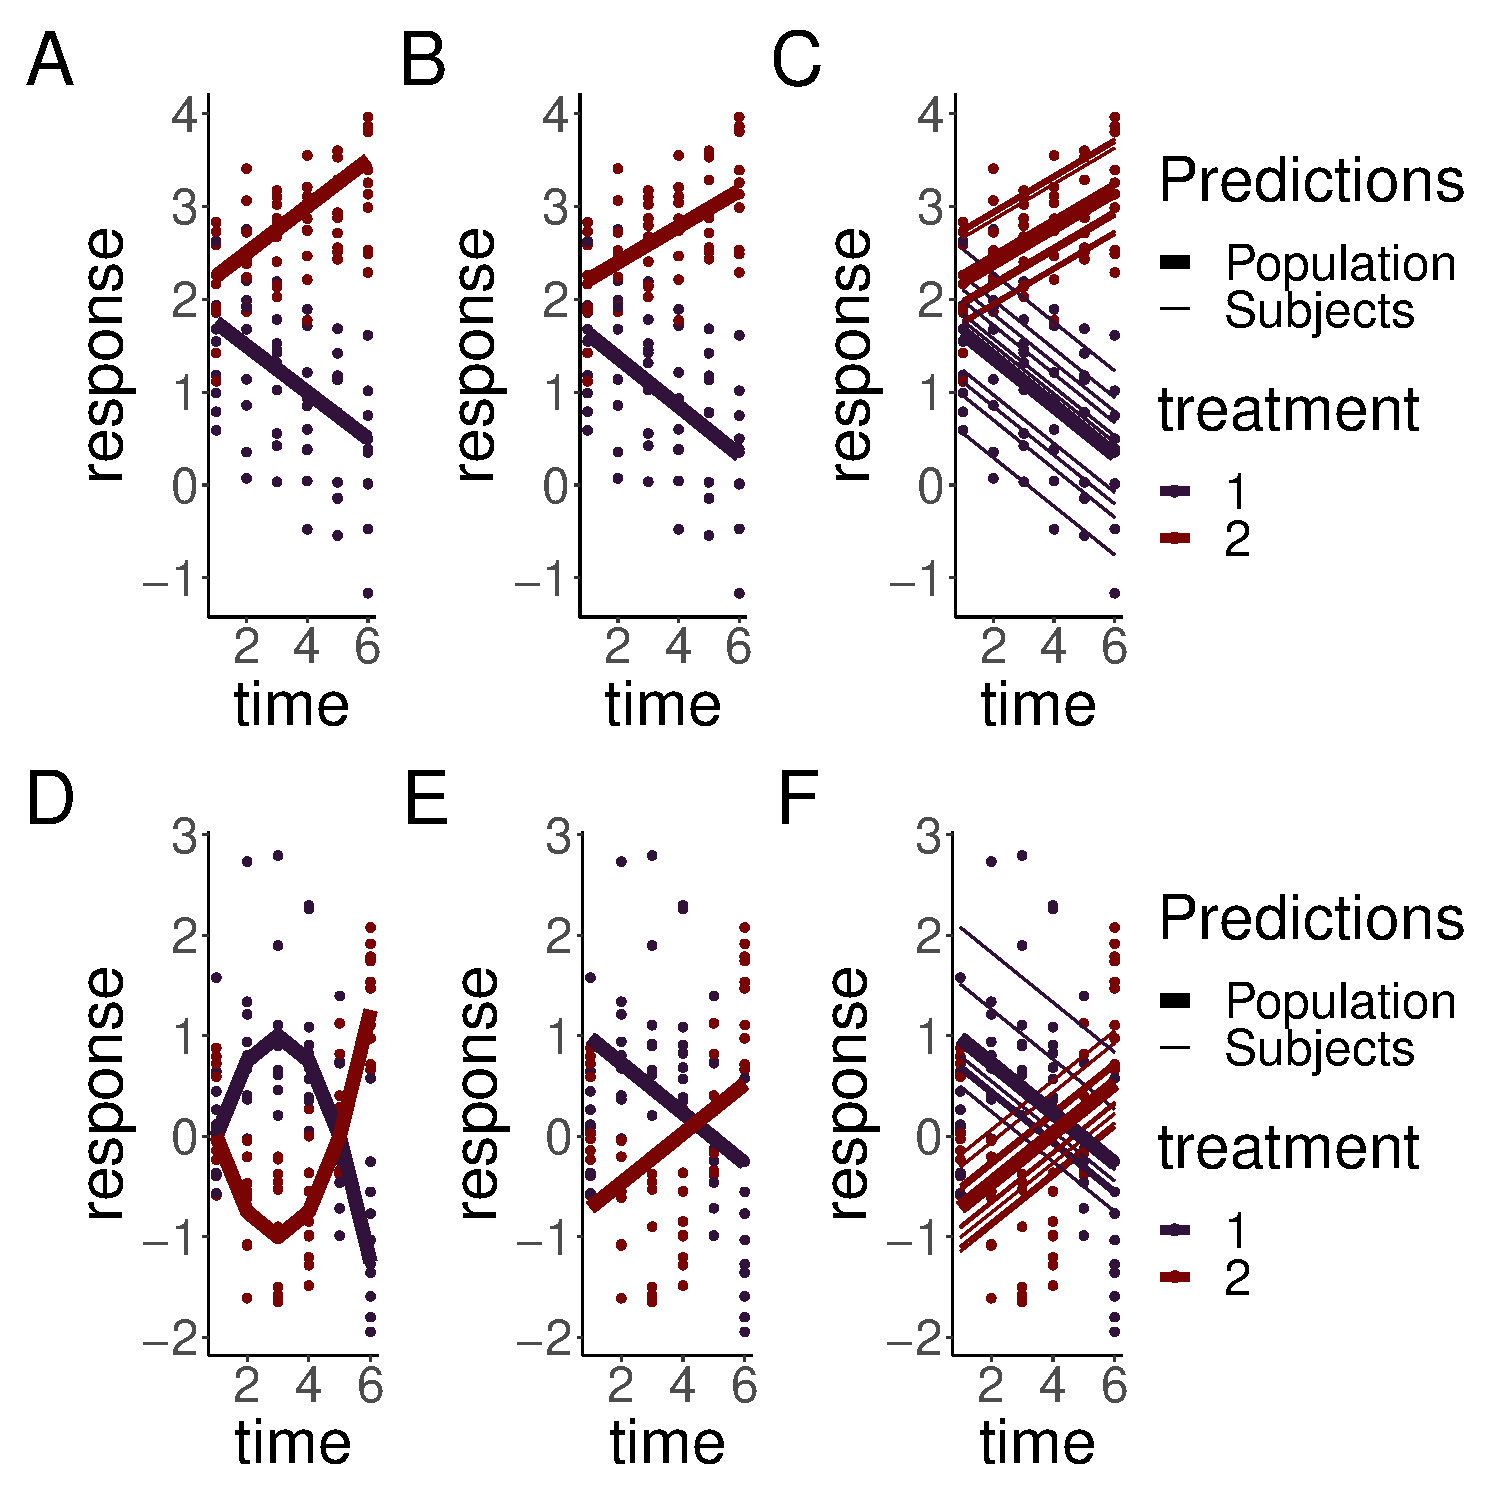
\includegraphics[width=0.75\linewidth,]{00-Full_document_files/figure-latex/l-q-response-1} 

}

\caption{Simulated responses from two groups with correlated errors using a LMEM and a rm-ANOVA model. Top row: linear response, bottom row: quadratic response. A: Simulated linear data with known mean response (thin lines) and individual responses (points) showing the dispersion of the data. D: Simulated quadratic data with known mean response (thin lines) and individual responses (points) showing the dispersion of the data. B,E: Estimates from the rm-ANOVA model for the mean group response (linear of quadratic). Points represent the original raw data. The rm-ANOVA model not only fails to pick the trend of the quadratic data (D) but also assigns a global estimate that does not take between-subject variation. C, F: Estimates from the LMEM in the linear and quadratic case. The LMEM incorporates a random effect for each subject, but this model and the rm-ANOVA model are unable to follow the trend of the data and grossly bias the initial estimates for each group in the quadratic case (bottom row).}\label{fig:l-q-response}
\end{figure}

The simulation shows that the fits produced by the LMEM and the rm-ANOVA model are good for linear data, as the predictions for the mean response are reasonably close to the ``truth'' of the simulated data (Figure \ref{fig:l-q-response}A). When the linearity and compound symmetry assumptions are met, the rm-ANOVA model approximates well the global trend by group (Figure \ref{fig:l-q-response}B). Note that because the LMEM incorporates \emph{random effects}, is able to provide estimates for each subject and a ``global'' estimate (Figure \ref{fig:l-q-response}C).

However, consider the case when the data follows a non-linear trend, such as the simulated data in Figure \ref{fig:l-q-response}D. Here, the mean response per group was simulated using a quadratic function, and errors and individual responses were produced as in Figure \ref{fig:l-q-response}A. The mean response in the simulated data with quadratic behavior changes in each group through the timeline, and the mean value is the same as the initial value by the fifth time point for each group. Fitting an rm-ANOVA model (Equation \eqref{eq:linear-model}) or a LMEM (Equation \eqref{eq:LMEM}) to this data produces the fit that appears in Figure \ref{fig:l-q-response}E, F.

Comparing the fitted responses of the LMEM and the rm-ANOVA models used in the simulated quadratic data (Figure \ref{fig:l-q-response}E, F) indicates that the models are not capturing the changes within each group. Specifically, note that the fitted mean response of both models shows that the change (increase for Treatment 1 or decrease for Treatment 2) in the response through time points 2 and 4 is not being captured. The LMEM is only able to account for between-subject variation by providing estimates for each subject (Figure \ref{fig:l-q-response}F), but both models are unable to capture the fact that the initial values are the same in each group, and instead fit non-parallel lines that have initial values that are markedly different from the ``true'' initial values in each case (compare Figure \ref{fig:l-q-response}D with Figure \ref{fig:l-q-response}E, F). If such a change has important physiological implications, both rm-ANOVA and LMEMs omit it from the fitted mean response. Thus, even though the model correctly detects a divergence between treatment groups, the exact nature of this difference is not correctly identified, limiting valuable inferences from the data.

This section has used simulation to better convey the limitations of linearity and correlation in the response in non-linear data. The models fitted to the simulated data were an rm-ANOVA model and a LMEM, where the main issue is the expected linear trend in the response. In the following section, we present generalized additive models (GAMs) as a data-driven alternative method to analyze longitudinal non-linear data that overcomes the linearity assumption.

\FloatBarrier

\hypertarget{GAM-theory}{%
\section{GAMs as a special case of Generalized Linear Models}\label{GAM-theory}}

\hypertarget{gams-and-basis-functions}{%
\subsection{GAMs and Basis Functions}\label{gams-and-basis-functions}}

Generalized linear models (GLMs) are a family of models (which include rm-ANOVA and LMEMs) that fit a linear response function to data that may not have normally distributed errors {[}\protect\hyperlink{ref-nelder1972}{50}{]}. In contrast, GAMs are a family of regression-based methods for estimating smoothly varying trends and are a broader class of models that contain the GLM family as a special case{[}\protect\hyperlink{ref-simpson2018}{34},\protect\hyperlink{ref-wood2017}{37},\protect\hyperlink{ref-hastie1987}{51}{]}. A GAM model can be written as:

\begin{equation}
  y_{ijt}=\beta_0+f(x_t\mid \beta_j)+\varepsilon_{ijt}
  \label{eq:GAM}
\end{equation}

Where \(y_{ijt}\) is the response at time \(t\) of subject \(i\) in group \(j\), \(\beta_0\) is the expected value at time 0, the change of \(y_{ijt}\) over time is represented by the \emph{smooth function} \(f(x_t\mid \beta_j)\) with inputs as the covariates \(x_t\) and parameters \(\beta_j\), and \(\varepsilon_{ijt}\) represents the residual error.

In contrast to the linear functions used to model the relationship between the covariates and the response in rm-ANOVA or LMEM, GAMs use more flexible \emph{smooth functions}. This approach is advantageous as it does not restrict the model to a linear relationship, although a GAM can estimate a linear relationship if the data is consistent with a linear response. One possible set of functions for \(f(x_t\mid \beta_j)\) that allow for non-linear responses are polynomials, but a major limitation is that polynomials create a ``global'' fit as they assume that the same relationship exists everywhere, which can cause problems with inference {[}\protect\hyperlink{ref-beck1998}{36}{]}. In particular, polynomial fits are known to show boundary effects because as \(t\) goes to \(\pm \infty\), \(f(x_t \mid \beta_j)\) goes to \(\pm \infty\) which is almost always unrealistic and causes bias at the endpoints of the time period.

The smooth functional relationship between the covariates and the response in GAMs is specified using a semi-parametric relationship that can be fit within the GLM framework, by using \emph{basis function} expansions of the covariates and by estimating random coefficients associated with these basis functions. A \emph{basis} is a set of functions that spans the mathematical space where the smooths that approximate \(f(x_t\mid \beta_j)\) exist {[}\protect\hyperlink{ref-simpson2018}{34}{]}. For the linear model in Equation \eqref{eq:linear-model}, the basis coefficients are \(\beta_1\), \(\beta_2\) and \(\beta_3\) and the basis vectors are \(time_t\), \(treatment_j\) and \(time_t \times treatment_j\). The basis function then, is the combination of basis coefficients and basis vectors that map the possible relationship between the covariates and the response {[}\protect\hyperlink{ref-hefley2017}{52}{]}, which in the case of Equation \eqref{eq:linear-model} is restricted to a linear family of functions. In the case of Equation \eqref{eq:GAM}, the basis functions are contained in the expression \(f(x_t\mid \beta_j)\), which means that the model allows for non-linear relationships among the covariates.

Splines (cubic, thin plate, etc.) are commonly used \emph{basis functions}; a cubic spline is a smooth curve constructed from cubic polynomials joined together in a manner that enforces smoothness, and thin plate regression splines are an optimized version that work well with noisy data {[}\protect\hyperlink{ref-simpson2018}{34},\protect\hyperlink{ref-wood2017}{37}{]}. Splines have a long history in solving semi-parametric statistical problems and are often a default choice to fit GAMs as they are a simple, flexible and powerful option to obtain smoothness {[}\protect\hyperlink{ref-wegman1983}{53}{]}. Therefore, this data-driven flexibility in GAMs overcomes the limitation that occurs in LMEMs and rm-ANOVA when the data is non linear.

To further clarify the concept of basis functions and smooth functions, consider the simulated response for Group 1 in Figure \ref{fig:l-q-response}C. The simplest GAM model that can be used to estimate such response is that of a single smooth term for the time effect; i.e., a model that fits a smooth to the trend of the group through time. The timeline can be divided in equally spaced \emph{knots}, each knot being a region where a different set of basis functions will be used. Because there are six timepoints for this group, five knots can be used. The model with five knots to construct the smooth term means that it will have four basis functions (plus one that corresponds to the intercept). The choice of basis functions is set using default values in the package \emph{mgcv} depending on the number of knots. In Figure \ref{fig:basis-plot}A, the four basis functions (and the intercept) are shown. Each of the basis functions is composed of six different points (because there are six points on the timeline). To control the ``wiggliness'' of the fit, each of the basis functions of Figure \ref{fig:basis-plot}A is weighted by multiplying it by a coefficient according to the matrix of Figure \ref{fig:basis-plot}B. The parameter estimates are penalized (shrunk towards 0) where the penalty reduces the ``wiggliness'' of the smooth fit to prevent overfitting. A weak penalty estimate will result in wiggly functions whereas a strong penalty estimate provides evidence that a linear response is appropriate.

To get the weighted basis functions, each basis (from Figure Figure \ref{fig:basis-plot}A) is multiplied by the corresponding coefficients in Figure \ref{fig:basis-plot}B, thereby increasing or decreasing the original basis functions. Figure \ref{fig:basis-plot}C shows the resulting weighted basis functions. Note that the magnitude of the weighting for the first basis function has resulted in a decrease of its overall value (because the coefficient for that basis function is less than 1). On the other hand, the third basis function has roughly doubled its value. Finally, the weighted basis functions are added at each timepoint to produce the smooth term. The resulting smooth term for the effect of \emph{time} is shown in Figure \ref{fig:basis-plot}D (orange line), along the simulated values per group, which appear as points.



\begin{figure}[H]

{\centering 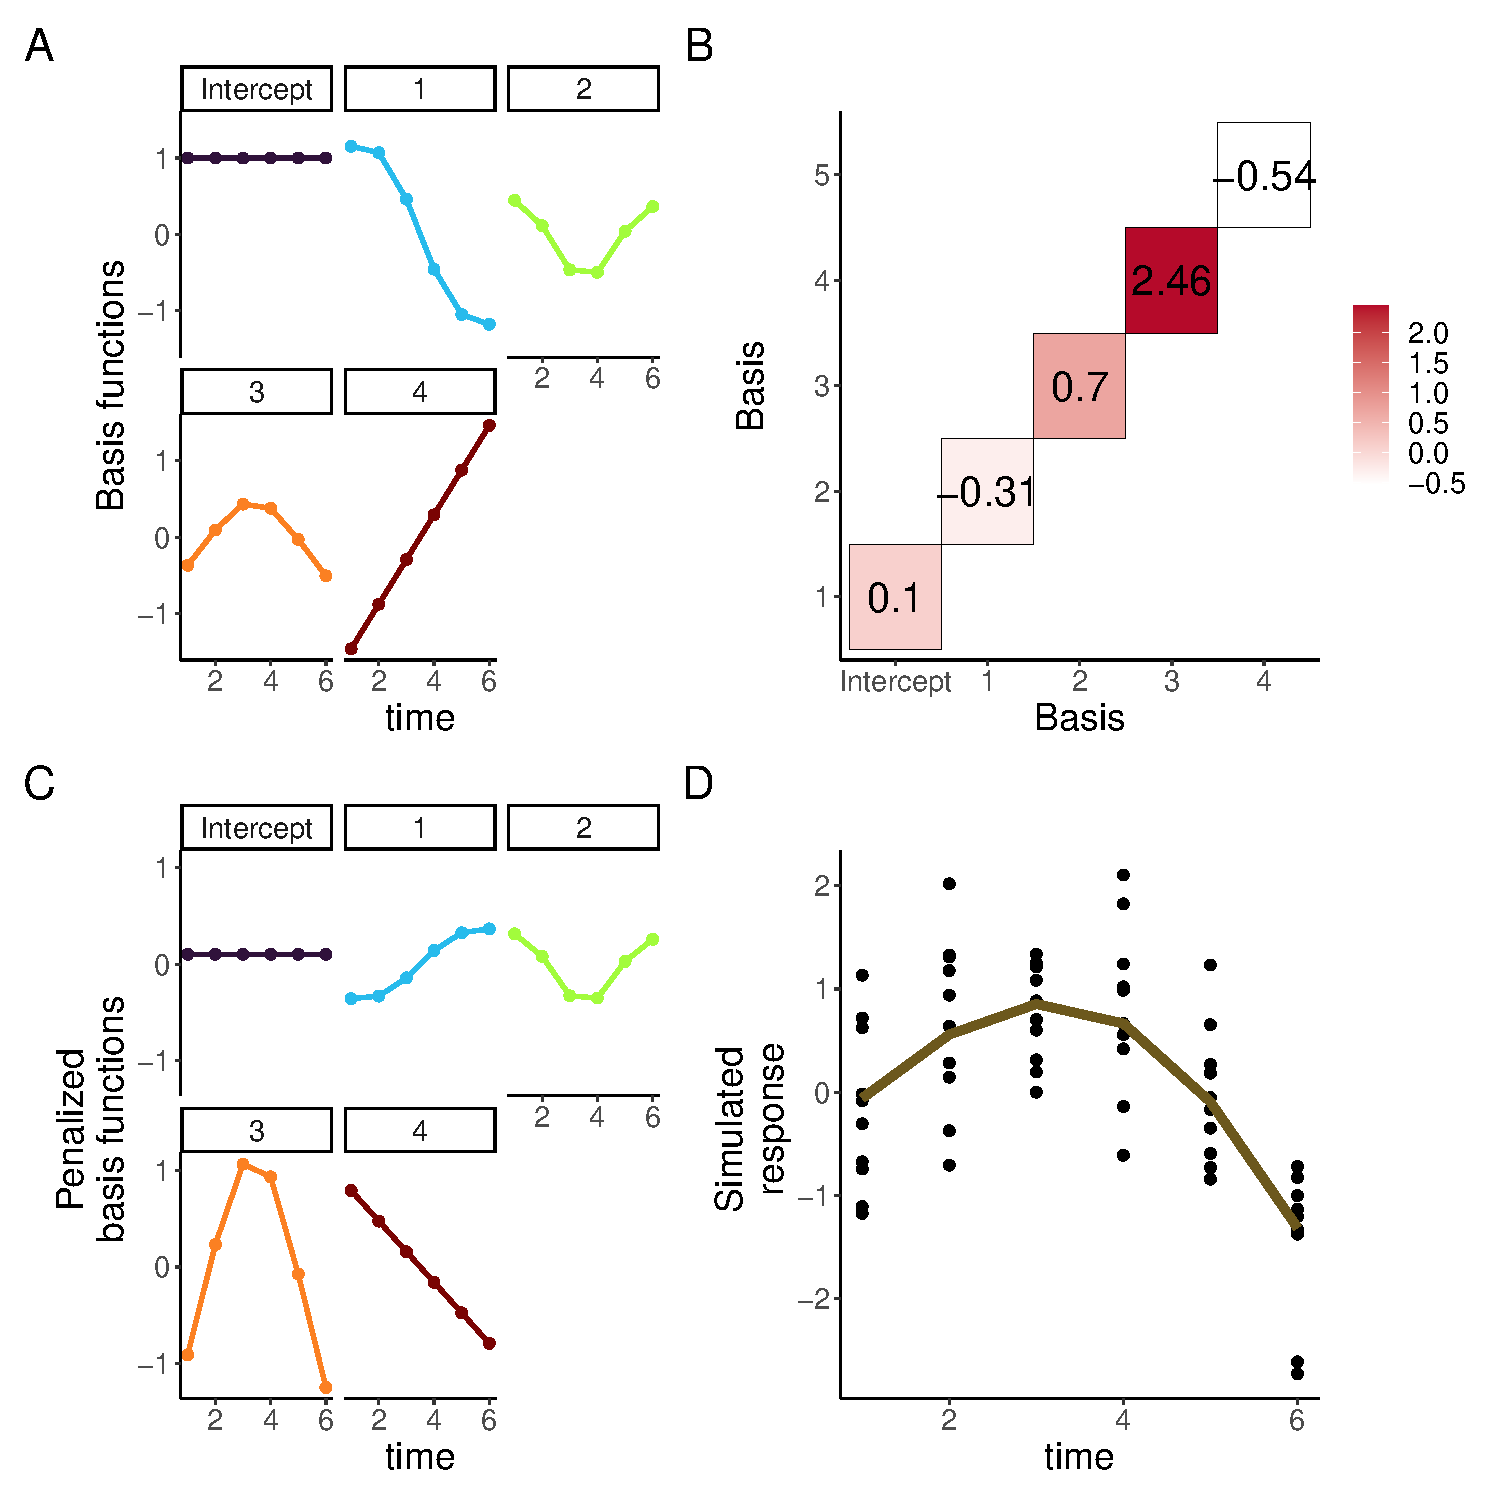
\includegraphics[width=0.75\linewidth,]{00-Full_document_files/figure-latex/basis-plot-1} 

}

\caption{Basis functions for a single smoother for time with five knots. A: Basis functions for a single smoother for time for the simulated data of Group 1 from Figure 2. B: Matrix of basis function weights. Each basis function is multiplied by a coefficient which can be positive or negative. The coefficient determines the overall effect of each basis in the final smoother. C: Weighted basis functions. Each of the four basis functions of panel A has been weighted by the corresponding coefficient shown in Panel B. Note the corresponding increase (or decrease) in magnitude of each weighted basis function. D: Smoother for time and original data points. The smoother (line) is the result of the sum of each weighted basis function at each time point, with simulated values for the group shown as points.}\label{fig:basis-plot}
\end{figure}

\hypertarget{a-bayesian-interpretation-of-gams}{%
\section{A Bayesian interpretation of GAMs}\label{a-bayesian-interpretation-of-gams}}

Bayes' theorem states that the probability of an event can be calculated using prior knowledge or belief {[}\protect\hyperlink{ref-mcelreath2018}{54}{]}. In the case of non-linear data, the belief that the \emph{true} trend of the data is likely to be smooth rather than ``wiggly'' introduces the concept of a prior distribution for wiggliness (and therefore a Bayesian view) of GAMs {[}\protect\hyperlink{ref-wood2017}{37}{]}. GAMs are considered ``empirical'' Bayesian models because the smoothing parameters are estimated from the data (and not from a prior distribution as in the ``Full Bayes'' case) {[}\protect\hyperlink{ref-miller2019}{55}{]}. Moreover, the use of the restricted maximum likelihood (REML) to estimate the smoothing parameters gives an empirical estimate of the smooth model {[}\protect\hyperlink{ref-pedersen2019}{33},\protect\hyperlink{ref-laird1982}{56}{]}. Therefore, the confidence intervals calculated for the smooth terms using the package \emph{mgcv} are considered empirical Bayesian posterior credible intervals {[}\protect\hyperlink{ref-pedersen2019}{33}{]}, which have good ``frequentist'' coverage (pointwise coverage or ``single point'' coverage), and \emph{across the function} coverage {[}\protect\hyperlink{ref-wood2017}{37}{]}. This last part means that contrary to a pointwise coverage (where the coverage of the interval is correct for a single point) the estimated confidence intervals for the smooths will contain \emph{on average} the true function of the data 95\% of the time across the entire timeline (in the case of longitudinal data for which smooths are calculated), which allows to obtain better inference from the model. In-depth theory of the Bayesian interpretation of GAMs is beyond the scope of this paper, but can be found in {[}\protect\hyperlink{ref-simpson2018}{34},\protect\hyperlink{ref-wood2017}{37},\protect\hyperlink{ref-miller2019}{55}{]} and {[}\protect\hyperlink{ref-marra2012}{57}{]}. With this brief introduction to the Bayesian interpretation of GAMs, we henceforth refer to the confidence intervals for the smooths in GAMs as ``empirical Bayesian'' through the rest of this paper.

\FloatBarrier

\hypertarget{longitudinal-GAMs}{%
\section{The analyisis of longitudinal biomedical data using GAMs}\label{longitudinal-GAMs}}

The previous sections provided the basic framework to understand the GAM framework and how these models are more advantageous to analyze non-linear longitudinal data when compared to rm-ANOVA or LMEMs. This section will use simulation to present the practical implementation of GAMs for longitudinal biomedical data using \(\textsf{R}\) and the package \passthrough{\lstinline!mgcv!}. The code for the simulated data and figures, and a brief guide for model selection and diagnostics appear in the Appendix.

\hypertarget{simulated-data}{%
\subsection{Simulated data}\label{simulated-data}}

The simulated data is based on the reported longitudinal changes in oxygen saturation (\(\mbox{StO}_2\)) in subcutaneous tumors that appear in Figure 3C in {[}\protect\hyperlink{ref-vishwanath2009}{16}{]}. In the paper, diffuse reflectance spectroscopy was used to quantify \(\mbox{StO}_2\) changes in both groups at the same time points (days 0, 2, 5, 7 and 10). In the ``Treatment'' group (chemotherapy) an increase in \(\mbox{StO}_2\) is observed through time, while a decrease is seen in the ``Control'' (saline) group. Following the reported trend, we simulated 10 normally distributed observations at each time point with a standard deviation (SD) of 10\% (matching the SD in the original paper).
The simulated and real data appear in Figure \ref{fig:sim-smooth-plot}A and the inset, respectively.

\hypertarget{an-interaction-gam-for-longitudinal-data}{%
\subsection{An interaction GAM for longitudinal data}\label{an-interaction-gam-for-longitudinal-data}}

An interaction effect is typically the main interest in longitudinal biomedical data, as it takes into account treatment, time, and their combination. In a practical sense, when a GAM is implemented for longitudinal data, a smooth can be added to the model for the \emph{time} effect to account for the repeated measures over time. Although specific methods of how GAMs model correlation structures is a topic beyond the scope of this paper, it suffices to say that GAMs are flexible and can handle correlation structures beyond compound symmetry. A detailed description on basis functions and correlations can be found in {[}\protect\hyperlink{ref-hefley2017}{52}{]}.

For the data in Figure \ref{fig:sim-smooth-plot}, A the main effect of interest is how \(\mbox{StO}_2\) changes over time for each treatment. To estimate this, the model incorporates independent smooths for \emph{Group} and \emph{Day}, respectively. The main thing to consider is that model syntax accounts for the fact that one of the variables is numeric (\emph{Day}) and the other is a factor (\emph{Group}). Because the smooths are centered at 0, the factor variable needs to be specified as a parametric term in order to identify any differences between the groups. Using \(\textsf{R}\) and the package \passthrough{\lstinline!mgcv!} the model syntax is:

\passthrough{\lstinline!m1 <- gam(StO2\_sim \~ Group + s(Day, by=Group, k=5), method='REML, data = dat\_sim)!}

This syntax specifies that \passthrough{\lstinline!m1!} will store the model, and that the change in the simulated oxygen saturation (\passthrough{\lstinline!StO2\_sim!}) is modeled using independent smooths over \passthrough{\lstinline!Day!} for each \passthrough{\lstinline!Group!} (the parenthesis preceded by \passthrough{\lstinline!s!}) using 5 knots. The smooth is constructed by default using thin plate regression splines, but other splines can be used if desired, including Gaussian process smooths {[}\protect\hyperlink{ref-simpson2018}{34}{]}. The parametric term \passthrough{\lstinline!Group!} is added to quantify overall mean differences in the effect of treatment between groups, and the \passthrough{\lstinline!method!} chosen to estimate the smoothing parameters is the restricted maximum likelihood (REML) {[}\protect\hyperlink{ref-wood2017}{37}{]}. When the smooths are plotted over the raw data, it is clear that the model has been able to capture the trend of the change of \(\mbox{StO}_2\) for each group across time (Figure \ref{fig:sim-smooth-plot}B). Model diagnostics can be obtained using the \passthrough{\lstinline!gam.check!} function, and the function \passthrough{\lstinline!appraise!} from the package \emph{gratia} {[}\protect\hyperlink{ref-gratia}{58}{]}. A guide for model selection and diagnostics is in the \protect\hyperlink{workflow}{Appendix}, and an in-depth analysis can be found in {[}\protect\hyperlink{ref-wood2017}{37}{]} and {[}\protect\hyperlink{ref-harezlak2018}{59}{]}.

One question that might arise at this point is ``what is the fit that an rm-ANOVA model produces for the simulated data?'' The rm-ANOVA model, which corresponds to Equation \eqref{eq:linear-model} is presented in Figure \ref{fig:sim-smooth-plot}C. This is a typical case of model misspecification: The slopes of each group are different, which would lead to a \emph{p-value} indicating significance for the treatment and time effects, but the model is not capturing the changes that occur at days 2 and between days 5 and 7, whereas the GAM model is able to reliably estimate the trend over all timepoints (Figure \ref{fig:sim-smooth-plot}B) .

Because GAMs do not require equally-spaced or complete observations for all subjects, they are advantageous to analyze longitudinal data where missingness exists. The rationale behind this is that GAMs are able to pick the trend in the data even when some observations are missing. However, this usually causes the resulting smooths to have wider confidence intervals and less ability to pick certain trends. Consider the simulated \(\mbox{StO}_2\) values from Figure \ref{fig:sim-smooth-plot}B. If 40\% of the total observations are randomly deleted and the same interaction GAM fitted for the complete dataset is used, the resulting smooths are still able to show a different trend for each group, but because the empirical Bayesian credible intervals for the smooths overlap during the first 3 days with fewer data points, the trend is less pronounced than in the full dataset (Figure \ref{fig:sim-smooth-plot}D). Although the confidence intervals have increased for both smooths, the model still shows different trends with as little as 4 observations per group at certain time points.



\begin{figure}[H]

{\centering 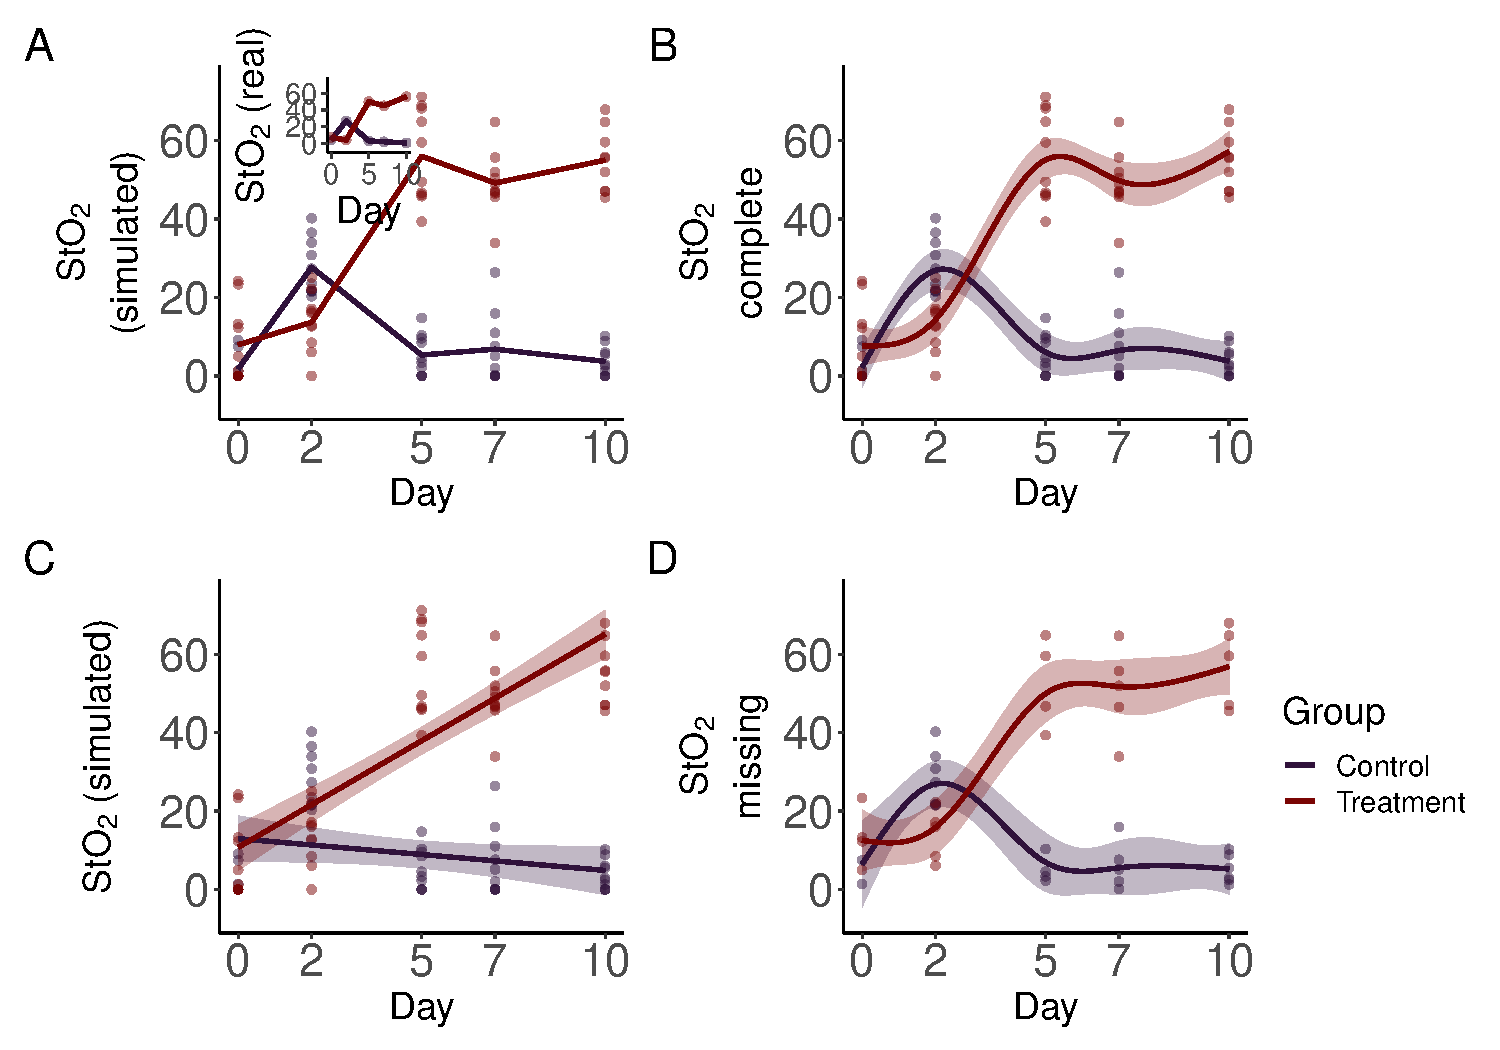
\includegraphics[width=0.75\linewidth,]{00-Full_document_files/figure-latex/sim-smooth-plot-1} 

}

\caption{Simulated data and smooths for oxygen saturation in tumors. A: Simulated data that follows previously reported trends (inset) in tumors under chemotherapy (Treatment) or saline (Control) treatment. Simulated data is from a normal distribution with standard deviation of 10\% with 10 observations per time point. Lines indicate mean oxygen saturation B: Smooths from the GAM model for the full simulated data with interaction of Group and Treatment. Lines represent trends for each group, shaded regions are 95\% confidence intervals. C: The rm-ANOVA model for the simulated data, which does not capture the changes in each group over time. D: Smooths for the GAM model for the simulated data with 40\% of its observations missing. Lines represent trends for each group, shaded regions are 95\% empirical Bayesian confidence intervals.}\label{fig:sim-smooth-plot}
\end{figure}



\begin{figure}[H]

{\centering 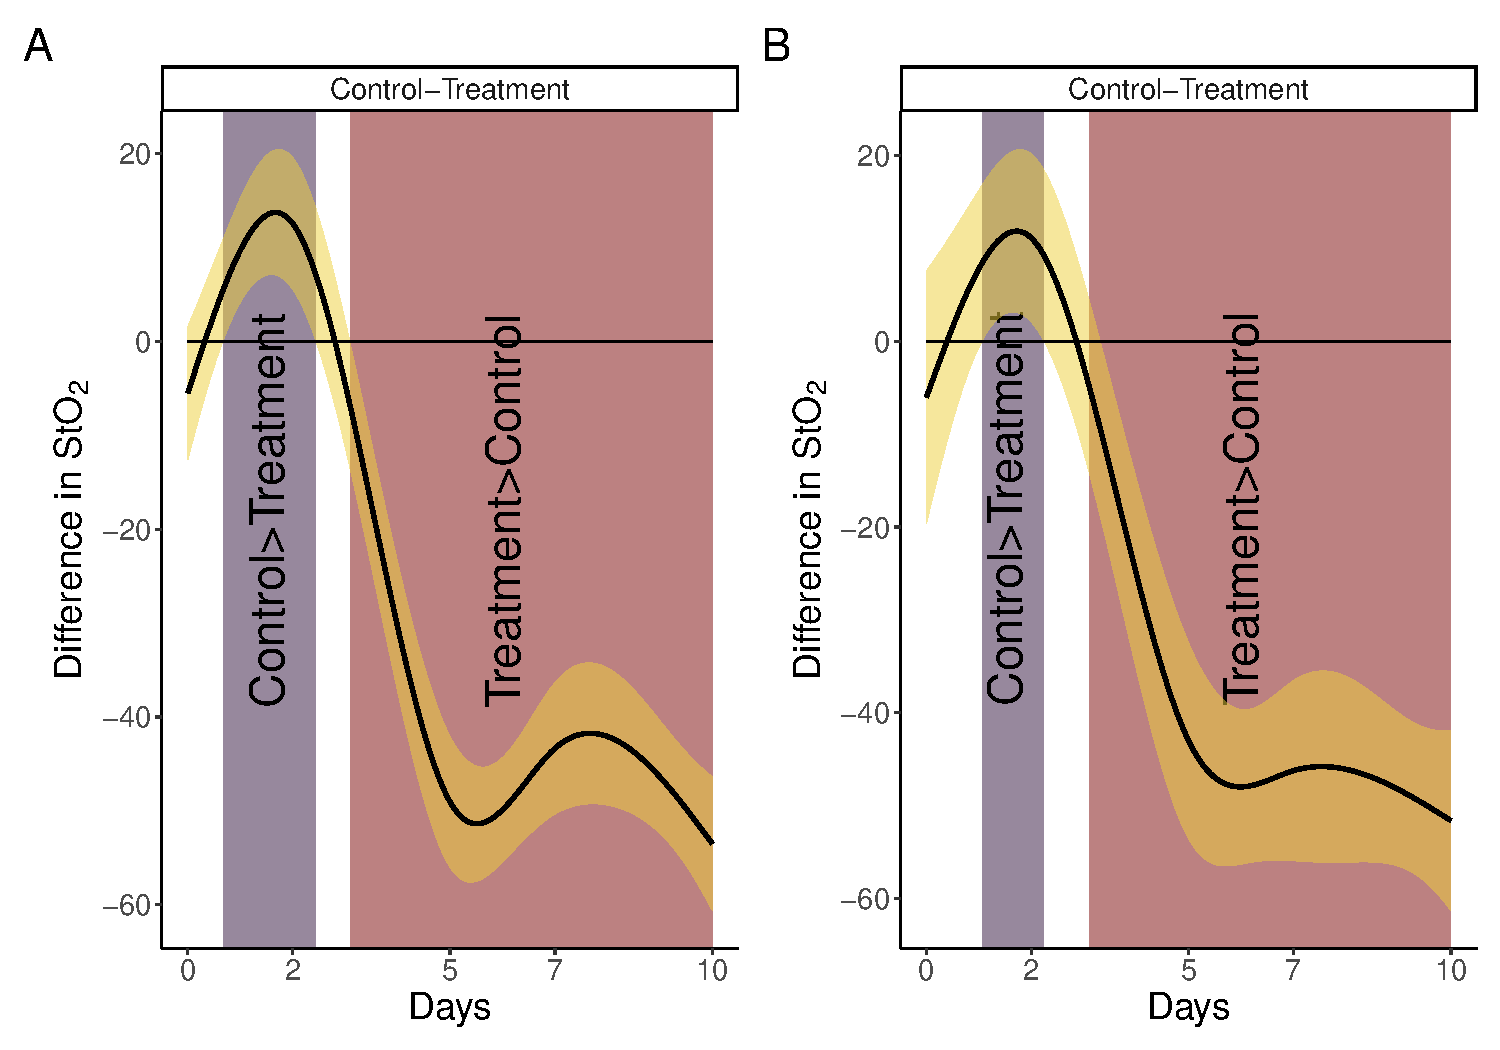
\includegraphics[width=0.75\linewidth,]{00-Full_document_files/figure-latex/plot-pairwise-comp-1} 

}

\caption{Pairwise comparisons for smooth terms. A: Pairwise comparisons for the full dataset. B: Pairwise comparisons for the dataset with missing observations. Significant differences exist where the 95\% empirical Bayesian credible interval does not cover 0. In both cases the effect of treatment is significant after day 3.}\label{fig:plot-pairwise-comp}
\end{figure}

\hypertarget{GAM-significance}{%
\subsection{Determination of significance in GAMs for longitudinal data}\label{GAM-significance}}

At the core of a biomedical longitudinal study lies the question of a significant difference between the effect of two or more treatments in different groups. Whereas in rm-ANOVA a \emph{post-hoc} analysis is required to answer such question by calculating some \emph{p-values} after multiple comparisons, GAMs can use a different approach to estimate significance. In essence, the idea behind the estimation of significance in GAMs across different treatment groups is that if the \emph{difference} between the empirical Bayesian confidence intervals of the fitted smooths for such groups is non-zero, then a significant difference exists at that time point(s). The absence of a \emph{p-value} in this case might seem odd, but the empirical Bayesian confidence interval interpretation can be conceptualized in the following manner: Different trends in each group are an indication of an effect by the treatment. This is what happens for the simulated data in Figure \ref{fig:sim-smooth-plot}A, where the chemotherapy causes \(\mbox{StO}_2\) to increase over time.

With this expectation of different trends in each group, computing the difference between the trends will identify if the observed change is significant. The difference between groups with similar trends is likely to yield zero, which would indicate that the treatment is not causing a change in the response in one of the groups (assuming the other group is a Control or Reference group).

Consider the calculation of pairwise differences for the smooths in Figure \ref{fig:sim-smooth-plot}B and Figure \ref{fig:sim-smooth-plot}D. Figure \ref{fig:plot-pairwise-comp} shows the comparison between each treatment group for the full and missing datasets. Here, the ``Control'' group is used as the reference to which ``Treatment'' group is being compared. Of notice, the pairwise comparison has been set on the response scale (see Appendix for code details), because otherwise the comparison appears shifted and is not intuitively easy to relate to the original data.

With this correction in mind, the shaded regions over the confidence interval (where it does not cover 0) indicate the time interval where each group has a higher effect than the other. Notice that the shaded region between days 0 and \(\approx\) 2 for the full dataset indicates that through that time, the ``Control'' group has higher mean \(\mbox{StO}_2\), but as therapy progresses the effect is reversed and by \(\approx\) 3 day it is the ``Treatment'' group the one that on average, has greater \(\mbox{StO}_2\). This would suggest that the effect of chemotherapy in the ``Treatment'' group becomes significant after day 3 for the given model. Moreover, notice that although there is no actual measurement at day 3, the model is capable of providing an estimate of when the shift in mean \(\mbox{StO}_2\) occurs.

On the data with missing observations (Figure \ref{fig:sim-smooth-plot}D), the empirical Bayesian credible intervals of the smooths overlap between days 0 and 3. Consequently, the smooth pairwise comparison (Figure \ref{fig:plot-pairwise-comp}B) shows that there is no evidence of a significant difference between the groups during that period, but is still able to pick the change on day 3 as the full dataset smooth pairwise comparison.

In a sense, the pairwise smooth comparison is more informative than a \emph{post-hoc} \emph{p-value}. For biomedical studies, the smooth comparison is able to provide an estimate of \emph{when} and by \emph{how much} a biological process becomes significant. This is advantageous because it can help researchers gain insight on metabolic changes and other biological processes that can be worth examining, and can help refine the experimental design of future studies in order to obtain measurements at time points where a significant change might be expected.

\FloatBarrier

\hypertarget{discussion}{%
\section{Discussion}\label{discussion}}

Biomedical longitudinal non-linear data is particularly challenging to analyze due to the likelihood of missing observations and different correlation structures in the data, which limit the use of rm-ANOVA. Although LMEMs have started to replace rm-ANOVA as the choice to analyze biomedical data, both methods yield biased estimates when they are used to fit non-linear data as we have visually demonstrated in Section \ref{simulation}. This ``model misspecification'' error, also is known as a ``Type III'' error {[}\protect\hyperlink{ref-dennis2019}{17}{]} is particularly important because although the \emph{p-value} is the common measure of statistical significance, the validity of its interpretation is determined by the agreement of the data and the model. Guidelines for statistical reporting in biomedical journals exist (the SAMPL guidelines) {[}\protect\hyperlink{ref-lang2015}{60}{]} but they have not been widely adopted and in the case of longitudinal data, we consider that researchers would benefit from reporting a visual assessment of the correspondence between the model fit and the data, instead of merely relying on a \(R^2\) value.

In this paper we have presented GAMs as a suitable method to analyze non-linear longitudinal data. It is interesting to note that although GAMs are a well established method to analyze temporal data in different fields (among which are palaeoecology, geochemistry, and ecology) {[}\protect\hyperlink{ref-pedersen2019}{33},\protect\hyperlink{ref-hefley2017}{52}{]} they are not routinely used in biomedical research despite an early publication from Hastie and Tibshirani that demonstrated their use in medical research {[}\protect\hyperlink{ref-hastie1995}{61}{]}. This is possibly due to the fact that the theory behind GAMs can seem very different from that of rm-ANOVA and LMEMs, but the purpose of Section \ref{GAM-theory} is to demonstrate that at its core the theory quite simple: Instead of using a linear relationship to model the response (as rm-ANOVA and LMEMs do), GAMs use basis functions to build smooths that are capable of following non-linear trends in the data.

However, from a practical standpoint is equally important to demonstrate how GAMs are computationally implemented. We have provided an example on how GAMs can be fitted using simulated data that follows trends reported in biomedical literature {[}\protect\hyperlink{ref-vishwanath2009}{16}{]} using \(\textsf{R}\) and the package \emph{mgcv}{[}\protect\hyperlink{ref-wood2017}{37}{]} in Section \ref{longitudinal-GAMs}, while a basic workflow for model selection is in the \protect\hyperlink{workflow}{Appendix}. One of the features of GAMs is that their Bayesian interpretation allows to indicate differences between groups without the need of a \emph{p-value}, and in turn provide a time-based estimate of shifts in the response that can be directly tied to biological values as the pairwise smooth comparisons in Figure \ref{fig:plot-pairwise-comp} indicate. The model is therefore able to provide an estimate of significant change between the groups at time points were data was not directly measured even with missing data exists ( \(\approx\) day 3 in Figure \ref{fig:plot-pairwise-comp} A, B ), which can be used by researchers as feedback on experiment design and to further evaluate important biological changes in future studies.

We have used \(\textsf{R}\) as the software of choice for this paper because not only provides a fully developed environment to fit GAMs, but also eases simulation (which is becoming increasingly used for exploratory statistical analysis and power calculations) and provides powerful and convenient methods of visualization, which are key aspects that biomedical researchers might need to consider to make their work reproducible. In this regard, reproducibility is still an issue in biomedical research {[}\protect\hyperlink{ref-begley2015}{62},\protect\hyperlink{ref-weissgerber2018}{63}{]}, but it is becoming apparent that what other disciplines have experienced in this aspect is likely to impact sooner rather than later this field. Researchers need to plan on how they will make their data, code, and any other materials open and accessible as more journals and funding agencies recognize the importance and benefits of open science in biomedical research. We have made all the data and code used in this paper accessible, and we hope that this will encourage other researchers to do the same with future projects.

\FloatBarrier

\hypertarget{conclusion}{%
\section{Conclusion}\label{conclusion}}

We have presented GAMs as a method to analyze longitudinal biomedical data. Future directions of this work will include simulation-based estimations of statistical power using GAMs, as well as demonstrating the prediction capabilities of these models using large datasets.
By making the data and code used in this paper accessible, we hope to address the need of creating and sharing reproducible work in biomedical research.

\hypertarget{acknowledgements}{%
\section{Acknowledgements}\label{acknowledgements}}

This work was supported by the National Science Foundation Career Award (CBET 1751554, TJM) and the Arkansas Biosciences Institute.

\FloatBarrier

\begin{center}\rule{0.5\linewidth}{0.5pt}\end{center}

\newpage

\hypertarget{references}{%
\section{References}\label{references}}

\hypertarget{refs}{}
\begin{CSLReferences}{0}{0}
\leavevmode\hypertarget{ref-roblyer2011}{}%
\CSLLeftMargin{{[}1{]} }
\CSLRightInline{D. Roblyer, S. Ueda, A. Cerussi, W. Tanamai, A. Durkin, R. Mehta, D. Hsiang, J.A. Butler, C. McLaren, W.P. Chen, B. Tromberg, Optical imaging of breast cancer oxyhemoglobin flare correlates with neoadjuvant chemotherapy response one day after starting treatment, Proceedings of the National Academy of Sciences of the United States of America. 108 (2011) 14626--14631. \url{https://doi.org/10.1073/pnas.1013103108}.}

\leavevmode\hypertarget{ref-tank2020}{}%
\CSLLeftMargin{{[}2{]} }
\CSLRightInline{A. Tank, H.M. Peterson, V. Pera, S. Tabassum, A. Leproux, T. O'Sullivan, E. Jones, H. Cabral, N. Ko, R.S. Mehta, B.J. Tromberg, D. Roblyer, Diffuse optical spectroscopic imaging reveals distinct early breast tumor hemodynamic responses to metronomic and maximum tolerated dose regimens, Breast Cancer Research. 22 (2020) 1--10. \url{https://doi.org/doi:10.1186/s13058-020-01262-1}.}

\leavevmode\hypertarget{ref-pavlov2018}{}%
\CSLLeftMargin{{[}3{]} }
\CSLRightInline{M.V. Pavlov, T.I. Kalganova, Y.S. Lyubimtseva, V.I. Plekhanov, G.Y. Golubyatnikov, O.Y. Ilyinskaya, A.G. Orlova, P.V. Subochev, D.V. Safonov, N.M. Shakhova, A.V. Maslennikova, {Multimodal approach in assessment of the response of breast cancer to neoadjuvant chemotherapy}, {Journal of Biomedical Optics}. {23} (2018). \url{https://doi.org/\%7B10.1117/1.JBO.23.9.091410\%7D}.}

\leavevmode\hypertarget{ref-demidov2018}{}%
\CSLLeftMargin{{[}4{]} }
\CSLRightInline{V. Demidov, A. Maeda, M. Sugita, V. Madge, S. Sadanand, C. Flueraru, I.A. Vitkin, {Preclinical longitudinal imaging of tumor microvascular radiobiological response with functional optical coherence tomography}, {Scientific Reports}. {8} (2018). \url{https://doi.org/\%7B10.1038/s41598-017-18635-w\%7D}.}

\leavevmode\hypertarget{ref-ritter2001}{}%
\CSLLeftMargin{{[}5{]} }
\CSLRightInline{G. Ritter, L. Cohen, C. Williams, E. Richards, L. Old, S. Welt, {Serological analysis of human anti-human antibody responses in colon cancer patients treated with repeated doses of humanized monoclonal antibody A33}, {Cancer Research}. {61} (2001) 6851--6859.}

\leavevmode\hypertarget{ref-roth2017}{}%
\CSLLeftMargin{{[}6{]} }
\CSLRightInline{E.M. Roth, A.C. Goldberg, A.L. Catapano, A. Torri, G.D. Yancopoulos, N. Stahl, A. Brunet, G. Lecorps, H.M. Colhoun, {Antidrug antibodies in atients treated with alirocumab}, {New England Journal of Medicine}. {376} (2017) 1589--1590. \url{https://doi.org/\%7B10.1056/NEJMc1616623\%7D}.}

\leavevmode\hypertarget{ref-jones2018}{}%
\CSLLeftMargin{{[}7{]} }
\CSLRightInline{J.D. Jones, H.E. Ramser, A.E. Woessner, K.P. Quinn, {In vivo multiphoton microscopy detects longitudinal metabolic changes associated with delayed skin wound healing}, {Communications Biology}. {1} (2018). \url{https://doi.org/\%7B10.1038/s42003-018-0206-4\%7D}.}

\leavevmode\hypertarget{ref-skala2010}{}%
\CSLLeftMargin{{[}8{]} }
\CSLRightInline{M.C. Skala, A. Fontanella, L. Lan, J.A. Izatt, M.W. Dewhirst, Longitudinal optical imaging of tumor metabolism and hemodynamics, Journal of Biomedical Optics. 15 (2010). \url{https://doi.org/10.1117/1.3285584}.}

\leavevmode\hypertarget{ref-greening2018}{}%
\CSLLeftMargin{{[}9{]} }
\CSLRightInline{G.J. Greening, K.P. Miller, C.R. Spainhour, M.D. Cato, T.J. Muldoon, {Effects of isoflurane anesthesia on physiological parameters in murine subcutaneous tumor allografts measured via diffuse reflectance spectroscopy}, {Biomedical Optics Express}. {9} (2018) 2871--2886. \url{https://doi.org/\%7B10.1364/BOE.9.002871\%7D}.}

\leavevmode\hypertarget{ref-sio2016}{}%
\CSLLeftMargin{{[}10{]} }
\CSLRightInline{T.T. Sio, P.J. Atherton, B.J. Birckhead, D.J. Schwartz, J.A. Sloan, D.K. Seisler, J.A. Martenson, C.L. Loprinzi, P.C. Griffin, R.F. Morton, J.C. Anders, T.J. Stoffel, R.E. Haselow, R.B. Mowat, M.A.N. Wittich, J.D. Bearden III, R.C. Miller, {Repeated measures analyses of dermatitis symptom evolution in breast cancer patients receiving radiotherapy in a phase 3 randomized trial of mometasone furoate vs placebo (N06C4 {{[}}alliance{]})}, {Supportive Care in Cancer}. {24} (2016) 3847--3855. \url{https://doi.org/\%7B10.1007/s00520-016-3213-3\%7D}.}

\leavevmode\hypertarget{ref-kamstra2015}{}%
\CSLLeftMargin{{[}11{]} }
\CSLRightInline{J.I. Kamstra, P.U. Dijkstra, M. van Leeuwen, J.L.N. Roodenburg, J.A. Langendijk, {Mouth opening in patients irradiated for head and neck cancer: A prospective repeated measures study}, {Oral Oncology}. {51} (2015) 548--555. \url{https://doi.org/\%7B10.1016/j.oraloncology.2015.01.016\%7D}.}

\leavevmode\hypertarget{ref-wagenmakers2008}{}%
\CSLLeftMargin{{[}12{]} }
\CSLRightInline{E.-J. Wagenmakers, M. Lee, T. Lodewyckx, G.J. Iverson, Bayesian versus frequentist inference, in: H. Hoijtink, I. Klugkist, P.A. Boelen (Eds.), Bayesian Evaluation of Informative Hypotheses, Springer New York, New York, NY, 2008: pp. 181--207. \url{https://doi.org/10.1007/978-0-387-09612-4_9}.}

\leavevmode\hypertarget{ref-gueorguieva2004}{}%
\CSLLeftMargin{{[}13{]} }
\CSLRightInline{R. Gueorguieva, J.H. Krystal, {Move over ANOVA - Progress in analyzing repeated-measures data and its reflection in papers published in the archives of general psychiatry}, Archives of General Psychiatry. 61 (2004) 310--317. \url{https://doi.org/10.1001/archpsyc.61.3.310}.}

\leavevmode\hypertarget{ref-schober2018}{}%
\CSLLeftMargin{{[}14{]} }
\CSLRightInline{P. Schober, T.R. Vetter, Repeated measures designs and analysis of longitudinal data: If at first you do not succeed-try, try again, Anesthesia and Analgesia. 127 (2018) 569--575. \url{https://doi.org/10.1213/ane.0000000000003511}.}

\leavevmode\hypertarget{ref-pinheiro2006}{}%
\CSLLeftMargin{{[}15{]} }
\CSLRightInline{J. Pinheiro, D. Bates, {Mixed-effects models in S and S-PLUS}, Springer Science \& Business Media, 2006. https://doi.org/\url{https://doi.org/10.1007/b98882}.}

\leavevmode\hypertarget{ref-vishwanath2009}{}%
\CSLLeftMargin{{[}16{]} }
\CSLRightInline{K. Vishwanath, H. Yuan, W.T. Barry, M.W. Dewhirst, N. Ramanujam, Using optical spectroscopy to longitudinally monitor physiological changes within solid tumors, Neoplasia. 11 (2009) 889--900. \url{https://doi.org/10.1593/neo.09580}.}

\leavevmode\hypertarget{ref-dennis2019}{}%
\CSLLeftMargin{{[}17{]} }
\CSLRightInline{B. Dennis, J.M. Ponciano, M.L. Taper, S.R. Lele, {Errors in statistical inference under model misspecification: evidence, hypothesis testing, and AIC}, {Frontiers in Ecology and Evolution}. {7} (2019). \url{https://doi.org/\%7B10.3389/fevo.2019.00372\%7D}.}

\leavevmode\hypertarget{ref-wang2019}{}%
\CSLLeftMargin{{[}18{]} }
\CSLRightInline{B. Wang, Z. Zhou, H. Wang, X.M. Tu, C. Feng, {The p-value and model specification in statistics}, {General Psychiatry}. {32} (2019). \url{https://doi.org/\%7B10.1136/gpsych-2019-100081\%7D}.}

\leavevmode\hypertarget{ref-liu2010}{}%
\CSLLeftMargin{{[}19{]} }
\CSLRightInline{C. Liu, T.P. Cripe, M.-O. Kim, Statistical issues in longitudinal data analysis for treatment efficacy studies in the biomedical sciences, Molecular Therapy. 18 (2010) 1724--1730. \url{https://doi.org/10.1038/mt.2010.127}.}

\leavevmode\hypertarget{ref-halsey2015}{}%
\CSLLeftMargin{{[}20{]} }
\CSLRightInline{L.G. Halsey, D. Curran-Everett, S.L. Vowler, G.B. Drummond, {The fickle \(p\) value generates irreproducible results}, {Nature Methods}. {12} (2015) 179--185. \url{https://doi.org/\%7B10.1038/nmeth.3288\%7D}.}

\leavevmode\hypertarget{ref-abdi2010}{}%
\CSLLeftMargin{{[}21{]} }
\CSLRightInline{H. Abdi, {Holm's sequential Bonferroni procedure}, Encyclopedia of Research Design. 1 (2010) 1--8. \url{https://doi.org/10.4135/9781412961288.n178}.}

\leavevmode\hypertarget{ref-nakagawa2004}{}%
\CSLLeftMargin{{[}22{]} }
\CSLRightInline{S. Nakagawa, {A farewell to Bonferroni: the problems of low statistical power and publication bias}, {Behavioral Ecology}. {15} (2004) 1044--1045. \url{https://doi.org/\%7B10.1093/beheco/arh107\%7D}.}

\leavevmode\hypertarget{ref-gelman2012}{}%
\CSLLeftMargin{{[}23{]} }
\CSLRightInline{A. Gelman, J. Hill, M. Yajima, {Why we (usually) don't have to worry about multiple comparisons}, {Journal of Research on Educational Effectiveness}. {5} (2012) 189--211. \url{https://doi.org/\%7B10.1080/19345747.2011.618213\%7D}.}

\leavevmode\hypertarget{ref-albers2019}{}%
\CSLLeftMargin{{[}24{]} }
\CSLRightInline{C. Albers, {The problem with unadjusted multiple and sequential statistical testing}, {Nature Communications}. {10} (2019). \url{https://doi.org/\%7B10.1038/s41467-019-09941-0\%7D}.}

\leavevmode\hypertarget{ref-ugrinowitsch2004}{}%
\CSLLeftMargin{{[}25{]} }
\CSLRightInline{C. Ugrinowitsch, G.W. Fellingham, M.D. Ricard, Limitations of ordinary least squares models in analyzing repeated measures data, Medicine and Science in Sports and Exercise. 36 (2004) 2144--2148. \url{https://doi.org/10.1249/01.mss.0000147580.40591.75}.}

\leavevmode\hypertarget{ref-huynh1976}{}%
\CSLLeftMargin{{[}26{]} }
\CSLRightInline{H. Huynh, L.S. Feldt, {Estimation of the Box correction for degrees of freedom from sample data in randomized block and split-plot designs}, Journal of Educational Statistics. 1 (1976) 69--82. \url{https://doi.org/10.3102/10769986001001069}.}

\leavevmode\hypertarget{ref-greenhouse1959}{}%
\CSLLeftMargin{{[}27{]} }
\CSLRightInline{S.W. Greenhouse, S. Geisser, On methods in the analysis of profile data, Psychometrika. 24 (1959) 95--112. \url{https://doi.org/10.1007/bf02289823}.}

\leavevmode\hypertarget{ref-haverkamp2017}{}%
\CSLLeftMargin{{[}28{]} }
\CSLRightInline{N. Haverkamp, A. Beauducel, {Violation of the sphericity assumption and its effect on type-I error rates in repeated measures ANOVA and multi-level linear models (MLM)}, {Frontiers in Psychology}. {8} (2017). \url{https://doi.org/\%7B10.3389/fpsyg.2017.01841\%7D}.}

\leavevmode\hypertarget{ref-keselman2001}{}%
\CSLLeftMargin{{[}29{]} }
\CSLRightInline{H. Keselman, J. Algina, R. Kowalchuk, {The analysis of repeated measures designs: A review}, {British Journal of Mathematica \& Statistical Psychology}. {54} (2001) 1--20. \url{https://doi.org/\%7B10.1348/000711001159357\%7D}.}

\leavevmode\hypertarget{ref-charan2013}{}%
\CSLLeftMargin{{[}30{]} }
\CSLRightInline{Jaykaran. Charan, N. Kantharia, {How to calculate sample size in animal studies?}, Journal of Pharmacology and Pharmacotherapeutics. 4 (2013) 303--306. \url{https://doi.org/10.4103/0976-500X.119726}.}

\leavevmode\hypertarget{ref-barr2013}{}%
\CSLLeftMargin{{[}31{]} }
\CSLRightInline{D.J. Barr, R. Levy, C. Scheepers, H.J. Tily, {Random effects structure for confirmatory hypothesis testing: Keep it maximal}, {Journal of Memory and Language}. {68} (2013) 255--278. \url{https://doi.org/\%7B10.1016/j.jml.2012.11.001\%7D}.}

\leavevmode\hypertarget{ref-rose2012}{}%
\CSLLeftMargin{{[}32{]} }
\CSLRightInline{N.L. Rose, H.D. Yang, S.D. Turner, G.L. Simpson, {An assessment of the mechanisms for the transfer of lead and mercury from atmospherically contaminated organic soils to lake sediments with particular reference to Scotland, UK}, Geochimica Et Cosmochimica Acta. 82 (2012) 113--135. \url{https://doi.org/10.1016/j.gca.2010.12.026}.}

\leavevmode\hypertarget{ref-pedersen2019}{}%
\CSLLeftMargin{{[}33{]} }
\CSLRightInline{E.J. Pedersen, D.L. Miller, G.L. Simpson, N. Ross, Hierarchical generalized additive models in ecology: An introduction with mgcv, {PeerJ}. 7 (2019). \url{https://doi.org/10.7717/peerj.6876}.}

\leavevmode\hypertarget{ref-simpson2018}{}%
\CSLLeftMargin{{[}34{]} }
\CSLRightInline{G.L. Simpson, Modelling palaeoecological time series using generalised additive models, Frontiers in Ecology and Evolution. 6 (2018). \url{https://doi.org/10.3389/fevo.2018.00149}.}

\leavevmode\hypertarget{ref-yang2012}{}%
\CSLLeftMargin{{[}35{]} }
\CSLRightInline{L. Yang, G. Qin, N. Zhao, C. Wang, G. Song, {Using a generalized additive model with autoregressive terms to study the effects of daily temperature on mortality}, {BMC Medical Research Methodology}. {12} (2012). \url{https://doi.org/\%7B10.1186/1471-2288-12-165\%7D}.}

\leavevmode\hypertarget{ref-beck1998}{}%
\CSLLeftMargin{{[}36{]} }
\CSLRightInline{N. Beck, S. Jackman, Beyond linearity by default: Generalized additive models, American Journal of Political Science. (1998) 596--627.}

\leavevmode\hypertarget{ref-wood2017}{}%
\CSLLeftMargin{{[}37{]} }
\CSLRightInline{S.N. Wood, {Generalized additive models: An introduction with R, Second Edition}, CRC Press LLC, Philadelphia, PA, 2017.}

\leavevmode\hypertarget{ref-r}{}%
\CSLLeftMargin{{[}38{]} }
\CSLRightInline{R Core Team, R: A language and environment for statistical computing, R Foundation for Statistical Computing, Vienna, Austria, 2020. \url{https://www.R-project.org/}.}

\leavevmode\hypertarget{ref-wood2016}{}%
\CSLLeftMargin{{[}39{]} }
\CSLRightInline{S.N. Wood, N. Pya, B. Saefken, Smoothing parameter and model selection for general smooth models, {Journal of the American Statistical Association}. {111} (2016) 1548--1563. \url{https://doi.org/\%7B10.1080/01621459.2016.1180986\%7D}.}

\leavevmode\hypertarget{ref-west2014}{}%
\CSLLeftMargin{{[}40{]} }
\CSLRightInline{B.T. West, K.B. Welch, A.T. Galecki, Linear mixed models: A practical guide using statistical software, second edition, Taylor \& Francis, 2014. \url{https://books.google.com/books?id=hjT6AwAAQBAJ}.}

\leavevmode\hypertarget{ref-wolfinger1996}{}%
\CSLLeftMargin{{[}41{]} }
\CSLRightInline{R.D. Wolfinger, Heterogeneous variance: Covariance structures for repeated measures, Journal of Agricultural, Biological, and Environmental Statistics. 1 (1996) 205--230. \url{http://www.jstor.org/stable/1400366}.}

\leavevmode\hypertarget{ref-weiss2005}{}%
\CSLLeftMargin{{[}42{]} }
\CSLRightInline{R.E. Weiss, Modeling longitudinal data, Springer New York, 2005. \url{https://books.google.com/books?id=MQ/_bvWDPsEAC}.}

\leavevmode\hypertarget{ref-geisser1958}{}%
\CSLLeftMargin{{[}43{]} }
\CSLRightInline{S. Geisser, S.W. Greenhouse, {An extension of Box's results on the use of the \(F\) distribution in multivariate analysis}, The Annals of Mathematical Statistics. 29 (1958) 885--891. \url{https://doi.org/10.1214/aoms/1177706545}.}

\leavevmode\hypertarget{ref-maxwell2017}{}%
\CSLLeftMargin{{[}44{]} }
\CSLRightInline{S.E. Maxwell, H.D. Delaney, K. Kelley, Designing experiments and analyzing data: A model comparison perspective, third edition, Taylor \& Francis, 2017. \url{https://books.google.com/books?id=NmFQDwAAQBAJ}.}

\leavevmode\hypertarget{ref-molenberghs2004}{}%
\CSLLeftMargin{{[}45{]} }
\CSLRightInline{G. Molenberghs, H. Thijs, I. Jansen, C. Beunckens, M. Kenward, C. Mallinckrodt, R. Carroll, {Analyzing incomplete longitudinal clinical trial data}, {Biostatistics}. {5} (2004) 445--464. \url{https://doi.org/\%7B10.1093/biostatistics/kxh001\%7D}.}

\leavevmode\hypertarget{ref-scheffer2002}{}%
\CSLLeftMargin{{[}46{]} }
\CSLRightInline{J. Scheffer, Dealing with missing data, Research Letters in the Information and Mathematical Sciences. 3 (2002) 153--160.}

\leavevmode\hypertarget{ref-potthoff2006}{}%
\CSLLeftMargin{{[}47{]} }
\CSLRightInline{R.F. Potthoff, G.E. Tudor, K.S. Pieper, V. Hasselblad, {Can one assess whether missing data are missing at random in medical studies?}, {Statistical Methods in Medical Research}. {15} (2006) 213--234. \url{https://doi.org/\%7B10.1191/0962280206sm448oa\%7D}.}

\leavevmode\hypertarget{ref-ma2012}{}%
\CSLLeftMargin{{[}48{]} }
\CSLRightInline{Y. Ma, M. Mazumdar, S.G. Memtsoudis, Beyond repeated-measures analysis of variance advanced statistical methods for the analysis of longitudinal data in anesthesia research, {Regional Anesthesia and Pain Medicine}. {37} (2012) 99--105. \url{https://doi.org/\%7B10.1097/AAP.0b013e31823ebc74\%7D}.}

\leavevmode\hypertarget{ref-nlme}{}%
\CSLLeftMargin{{[}49{]} }
\CSLRightInline{J. Pinheiro, D. Bates, S. DebRoy, D. Sarkar, R Core Team, {nlme}: Linear and nonlinear mixed effects models, 2020. \url{https://CRAN.R-project.org/package=nlme}.}

\leavevmode\hypertarget{ref-nelder1972}{}%
\CSLLeftMargin{{[}50{]} }
\CSLRightInline{J.A. Nelder, R.W.M. Wedderburn, Generalized linear models, Journal of the Royal Statistical Society. Series A (General). 135 (1972) 370--384. \url{http://www.jstor.org/stable/2344614}.}

\leavevmode\hypertarget{ref-hastie1987}{}%
\CSLLeftMargin{{[}51{]} }
\CSLRightInline{T. Hastie, R. Tibshirani, Generalized additive models: Some applications, Journal of the American Statistical Association. 82 (1987) 371--386. \url{https://doi.org/10.1080/01621459.1987.10478440}.}

\leavevmode\hypertarget{ref-hefley2017}{}%
\CSLLeftMargin{{[}52{]} }
\CSLRightInline{T.J. Hefley, K.M. Broms, B.M. Brost, F.E. Buderman, S.L. Kay, H.R. Scharf, J.R. Tipton, P.J. Williams, M.B. Hooten, {The basis function approach for modeling autocorrelation in ecological data}, {Ecology}. {98} (2017) 632--646. \url{https://doi.org/\%7B10.1002/ecy.1674\%7D}.}

\leavevmode\hypertarget{ref-wegman1983}{}%
\CSLLeftMargin{{[}53{]} }
\CSLRightInline{E.J. Wegman, I.W. Wright, Splines in statistics, Journal of the American Statistical Association. 78 (1983) 351--365. \url{https://doi.org/10.1080/01621459.1983.10477977}.}

\leavevmode\hypertarget{ref-mcelreath2018}{}%
\CSLLeftMargin{{[}54{]} }
\CSLRightInline{R. McElreath, {Statistical rethinking: A Bayesian course with examples in R and Stan}, {Chapman and Hall/CRC}, 2018. \url{https://doi.org/10.1201/9781315372495}.}

\leavevmode\hypertarget{ref-miller2019}{}%
\CSLLeftMargin{{[}55{]} }
\CSLRightInline{D.L. Miller, Bayesian views of generalized additive modelling, arXiv Preprint arXiv:1902.01330. (2019).}

\leavevmode\hypertarget{ref-laird1982}{}%
\CSLLeftMargin{{[}56{]} }
\CSLRightInline{N.M. Laird, J.H. Ware, Random-effects models for longitudinal data, Biometrics. 38 (1982) 963--974. \url{http://www.jstor.org/stable/2529876}.}

\leavevmode\hypertarget{ref-marra2012}{}%
\CSLLeftMargin{{[}57{]} }
\CSLRightInline{G. Marra, S.N. Wood, Coverage properties of confidence intervals for generalized additive model components, {Scandinavian Journal of Statistics}. {39} (2012) 53--74. \url{https://doi.org/\%7B10.1111/j.1467-9469.2011.00760.x\%7D}.}

\leavevmode\hypertarget{ref-gratia}{}%
\CSLLeftMargin{{[}58{]} }
\CSLRightInline{G.L. Simpson, Gratia: Graceful 'ggplot'-based graphics and other functions for GAMs fitted using 'mgcv', 2020. \url{https://CRAN.R-project.org/package=gratia}.}

\leavevmode\hypertarget{ref-harezlak2018}{}%
\CSLLeftMargin{{[}59{]} }
\CSLRightInline{J. Harezlak, D. Ruppert, M.P. Wand, {Semiparametric Regression with R}, Springer New York, 2018. \url{https://doi.org/10.1007/978-1-4939-8853-2}.}

\leavevmode\hypertarget{ref-lang2015}{}%
\CSLLeftMargin{{[}60{]} }
\CSLRightInline{T.A. Lang, D.G. Altman, {Basic statistical reporting for articles published in Biomedical Journals: The ``Statistical Analyses and Methods in the Published Literature{''} or the SAMPL Guidelines}, INTERNATIONAL JOURNAL OF NURSING STUDIES. {52} (2015) 5--9. \url{https://doi.org/\%7B10.1016/j.ijnurstu.2014.09.006\%7D}.}

\leavevmode\hypertarget{ref-hastie1995}{}%
\CSLLeftMargin{{[}61{]} }
\CSLRightInline{T. Hastie, R. Tibshirani, Generalized additive models for medical research, {Statistical Methods in Medical Research}. 4 (1995) 187--196. \url{https://doi.org/10.1177/096228029500400302}.}

\leavevmode\hypertarget{ref-begley2015}{}%
\CSLLeftMargin{{[}62{]} }
\CSLRightInline{C.G. Begley, J.P.A. Ioannidis, {Reproducibility in Science Improving the Standard for Basic and Preclinical Research}, {Circulation Research}. {116} (2015) 116--126. \url{https://doi.org/\%7B10.1161/CIRCRESAHA.114.303819\%7D}.}

\leavevmode\hypertarget{ref-weissgerber2018}{}%
\CSLLeftMargin{{[}63{]} }
\CSLRightInline{T.L. Weissgerber, O. Garcia-Valencia, V.D. Garovic, N.M. Milic, S.J. Winham, {Meta-Research: Why we need to report more than 'Data were Analyzed by t-tests or ANOVA'}, Elife. 7 (2018) e36163. \url{https://doi.org/10.7554/eLife.36163}.}

\end{CSLReferences}

\hypertarget{appendix-appendix}{%
\appendix}


\hypertarget{code-for-manuscript-data}{%
\section{Code for Manuscript data}\label{code-for-manuscript-data}}

This section presents the code used to generate figures, models and simulated data from Sections 3 and 4 from the main manuscript.

\hypertarget{compound-symmetry-and-independent-errors-in-linear-and-quadratic-responses}{%
\subsection{Compound symmetry and independent errors in linear and quadratic responses}\label{compound-symmetry-and-independent-errors-in-linear-and-quadratic-responses}}

This section simulated linear and quadratic data in the same manner as in Section \ref{simulation}. The linear simulations using Figure \ref{fig:linear-cases-Appendix} show in panels A and D the simulated mean responses and individual data points. Panels C and G show a visual interpretation of ``correlation'' in the responses: In panel C, subjects that have a value of the random error \(\varepsilon\) either above or below the mean group response are more likely to have other observations that follow the same trajectory, thereby demonstrating correlation in the response. In panel G,because the errors are independent, there is no expectation that responses are likely to follow a similar pattern. Panels D and H show the predictions from the rm-ANOVA model.

The following code produces a more comprehensive exploration of Figure \ref{fig:l-q-response} in the main manuscript.

\begin{lstlisting}[language=R]
##########Section for calculations###########


## Example with linear response

#This function simulates data using a linear or quadratic mean response and each with correlated
#or uncorrelated errors. Each group has a different slope/concavity.
example <- function(n_time = 6, #number of time points
                    fun_type = "linear", #type of response
                    error_type = "correlated") {
  
  if (!(fun_type %in% c("linear", "quadratic")))
    stop('fun_type must be either "linear", or "quadratic"')
  if (!(error_type %in% c("correlated", "independent")))
    stop('fun_type must be either "correlated", or "independent"')
  
  
  x <- seq(1,6, length.out = n_time)
  
  #Create mean response matrix: linear or quadratic
  mu <- matrix(0, length(x), 2)
  # linear response
  if (fun_type == "linear") {
    mu[, 1] <- - (0.25*x)+2  
    mu[, 2] <- 0.25*x+2
  } else {
    # quadratic response (non-linear)
    
    mu[, 1] <-  -(0.25 * x^2) +1.5*x-1.25
    mu[, 2] <- (0.25 * x^2) -1.5*x+1.25
  }
  
  #create an array where individual observations per each time point for each group are to be stored. Currently using 10 observations per timepoint
  y <- array(0, dim = c(length(x), 2, 10))
  
  #Create array to store the "errors" for each group at each timepoint. The "errors" are the 
  #between-group variability in the response.
  errors <- array(0, dim = c(length(x), 2, 10))
  #create an array where 10 observations per each time point for each group are to be stored
  
  #The following cycles create independent or correlated responses. To each value of mu (mean response per group) a randomly generated error (correlated or uncorrelated) is added and thus the individual response is created.
  if (error_type == "independent") {
    ## independent errors
    for (i in 1:2) {
      for (j in 1:10) {
        errors[, i, j] <- rnorm(6, 0, 0.25)
        y[, i, j] <- mu[, i] + errors[, i, j]
      }
    }
  } else {
    for (i in 1:2) {     # number of treatments
      for (j in 1:10) {  # number of subjects
        # compound symmetry errors: variance covariance matrix
        errors[, i, j] <- rmvn(1, rep(0, length(x)), 0.1 * diag(6) + 0.25 * matrix(1, 6, 6))
        y[, i, j] <- mu[, i] + errors[, i, j]
      }
    }
  }    
  
  
  ## subject random effects
  
  ## visualizing the difference between independent errors and compound symmetry
  ## why do we need to account for this -- overly confident inference
  
#labeling y and errors  
  dimnames(y) <- list(time = x, 
                      treatment = 1:2, 
                      subject = 1:10)

  dimnames(errors) <- list(time = x, 
                           treatment = 1:2, 
                           subject = 1:10)
  
  #labeling the mean response
  dimnames(mu) <- list(time = x, 
                       treatment = 1:2)
  
  #convert y, mu and errors to  dataframes with time, treatment and subject columns
  dat <- as.data.frame.table(y, 
                             responseName = "y")
  dat_errors <- as.data.frame.table(errors, 
                                    responseName = "errors")
  dat_mu <- as.data.frame.table(mu, 
                                responseName = "mu")
  
  #join the dataframes to show mean response and errors per subject
  dat <- left_join(dat, dat_errors, 
                   by = c("time", "treatment", "subject"))
  dat <- left_join(dat, dat_mu, 
                   by = c("time", "treatment"))
  #add time
  dat$time <- as.numeric(as.character(dat$time))
  #label subjects per group
  dat <- dat %>%
    mutate(subject = factor(paste(subject, 
                                  treatment, 
                                  sep = "-")))
  
  
  ## repeated measures ANOVA 
  
  fit_anova <- lm(y ~ time + treatment + time * treatment, data = dat)
  
#LMEM: time and treatment interaction model, compound symmetry 
  fit_lme <- lme(y ~ treatment + time + treatment:time,
                 data = dat,
                 random = ~ 1 | subject,
                 correlation = corCompSymm(form = ~ 1 | subject)
  )
  
  #create a prediction frame where the model can be used for plotting purposes
  pred_dat <- expand.grid(
    treatment = factor(1:2), 
    time = unique(dat$time)
  )
  
  #add model predictions to the dataframe that has the simulated data
  dat$pred_anova <- predict(fit_anova)
  dat$pred_lmem <- predict(fit_lme)

  #return everything in a list
  return(list(
    dat = dat,
    pred_dat = pred_dat,
    fit_anova=fit_anova,
    fit_lme = fit_lme
  ))
}
##################Section for plotting#################################
#######################################################################
#This function will create the plots for either a "linear" or "quadratic" response

plot_example <- function(sim_dat) {
  ## Plot the simulated data (scatterplot)
  
  p1 <- sim_dat$dat %>%
    ggplot(aes(x = time, 
               y = y, 
               group = treatment, 
               color = treatment)
           ) +
    geom_point(show.legend=FALSE) +
    labs(y='response')+
    geom_line(aes(x = time, 
                  y = mu, 
                  color = treatment),
              show.legend=FALSE) +
    theme_classic() +
    theme(plot.title = element_text(size = 30, 
                                  face = "bold"),
        text=element_text(size=30))+
    thm
  
  #plot the simulated data with trajectories per each subject
  p2 <- sim_dat$dat %>%
    ggplot(aes(x = time, 
               y = y, 
               group = subject, 
               color = treatment)
           ) +
    geom_line(aes(size = "Subjects"),
              show.legend = FALSE) +
    # facet_wrap(~ treatment) +
    geom_line(aes(x = time, 
                  y = mu, 
                  color = treatment,
                  size = "Simulated Truth"), 
              lty = 1,show.legend = FALSE) +
    labs(y='response')+
    scale_size_manual(name = "Type", values=c("Subjects" = 0.5, "Simulated Truth" = 3)) +
    theme_classic()+
     theme(plot.title = element_text(size = 30, 
                                face = "bold"),
     text=element_text(size=30))+
    thm
  
  #plot the errors
   p3 <- sim_dat$dat %>%
    ggplot(aes(x = time, 
               y = errors,
               group = subject, 
               color = treatment)) +
    geom_line(show.legend=FALSE) +
     labs(y='errors')+
     theme_classic()+
     theme(plot.title = element_text(size = 30, 
                                  face = "bold"),
        text=element_text(size=30))+
    thm
  
   #plot the model predictions for rm-ANOVA
  p4 <- ggplot(sim_dat$dat, 
               aes(x = time, 
                   y = y, 
                   color = treatment)) +
    geom_point(show.legend=FALSE)+
    labs(y='response')+
    geom_line(aes(y = predict(sim_dat$fit_anova), 
                  group = subject, size = "Subjects"),show.legend = FALSE) +
    geom_line(data = sim_dat$pred_dat, 
              aes(y = predict(sim_dat$fit_anova, 
                              level = 0, 
                              newdata = sim_dat$pred_dat), 
                  size = "Population"),
              show.legend=FALSE) +
    guides(color = guide_legend(override.aes = list(size = 2)))+
    scale_size_manual(name = "Predictions", 
                      values=c("Subjects" = 0.5, "Population" = 3)) +
    theme_classic() +
    theme(plot.title = element_text(size = 30, 
                                  face = "bold"),
        text=element_text(size=30))+
    thm
   
   
   
   #plot the LMEM predictions
  p5 <- ggplot(sim_dat$dat, 
               aes(x = time, 
                   y = y, 
                   color = treatment)) +
    geom_point()+
    labs(y='response')+
    geom_line(aes(y = predict(sim_dat$fit_lme), 
                  group = subject, size = "Subjects")) +
    geom_line(data = sim_dat$pred_dat, 
              aes(y = predict(sim_dat$fit_lme, 
                              level = 0, 
                              newdata = sim_dat$pred_dat), 
                  size = "Population")) +
    guides(color = guide_legend(override.aes = list(size = 2)))+
    scale_size_manual(name = "Predictions", 
                      values=c("Subjects" = 0.5, "Population" = 3)) +
    theme_classic() +
    theme(plot.title = element_text(size = 30, 
                                  face = "bold"),
        text=element_text(size=30))+
    thm
  
  return((p1+p3+p2+p4+p5)+plot_layout(nrow=1)+plot_annotation(tag_levels = 'A')) 
  
    
}

txt<-18

#Store each plot in a separate object
A1<-plot_example(example(fun_type = "linear", error_type = "correlated")) 

B1<-plot_example(example(fun_type = "linear", error_type = "independent")) 
  
C1<-plot_example(example(fun_type = "quadratic", error_type = "correlated")) 
  
D1<-plot_example(example(fun_type = "quadratic", error_type = "independent")) 
\end{lstlisting}



\begin{figure}[H]
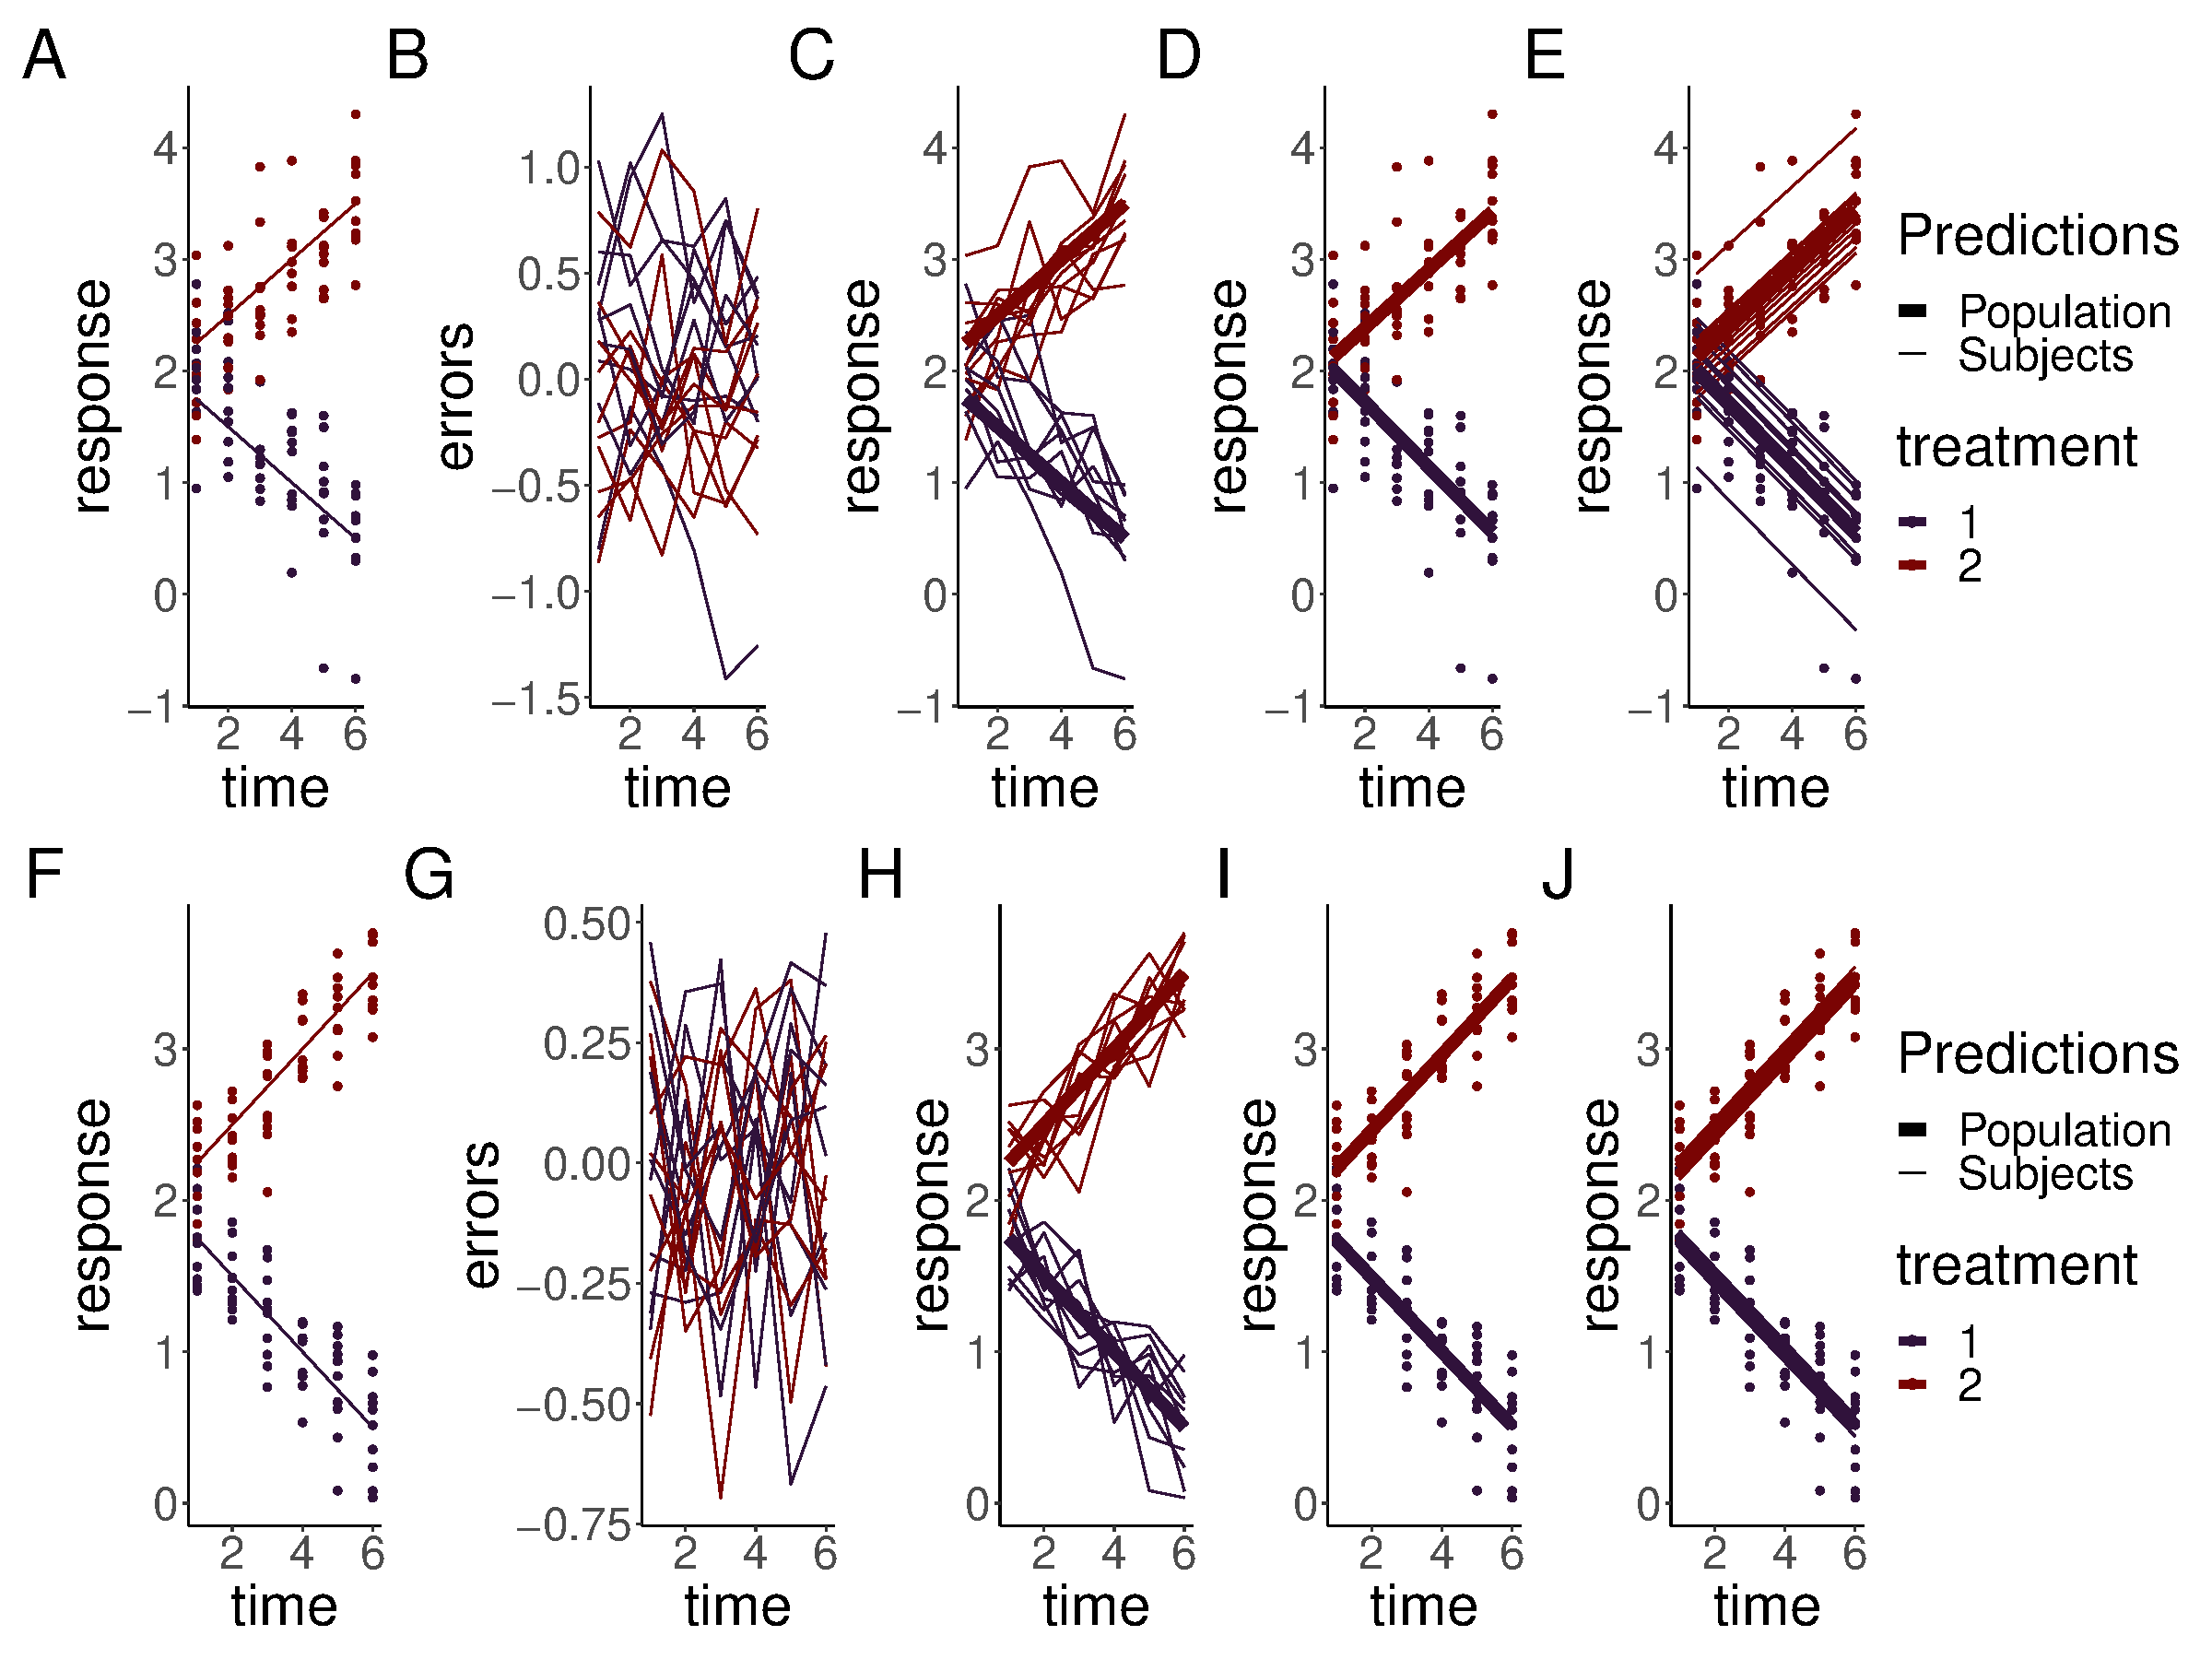
\includegraphics{00-Full_document_files/figure-latex/linear-cases-Appendix-1} \caption{Simulated linear responses from two groups with correlated (top row) or independent (bottom row) errors using a rm-ANOVA model and a LMEM. A, F:Simulated data with known mean response and individual responses (points) showing the dispersion of the data. B,G: Generated errors showing the difference in the behavior of correlated and independent errors. C,H: Simulated data with thin lines representing individual trajectories. D,I: Estimations from the rm-ANOVA model for the mean group response. E, J: Estimations from the LMEM for the mean group response and individual responses (thin lines). In all panels, thick lines are the predicted mean response per group, thin lines are the random effects for each subject and points represent the original raw data. Both rm-ANOVA and the LMEM are able to capture the trend of the data.}\label{fig:linear-cases-Appendix}
\end{figure}

For the quadratic response case, Figure \ref{fig:quadratic-cases-Appendix} shows the simulated responses using compound symmetry and independent errors.



\begin{figure}[H]
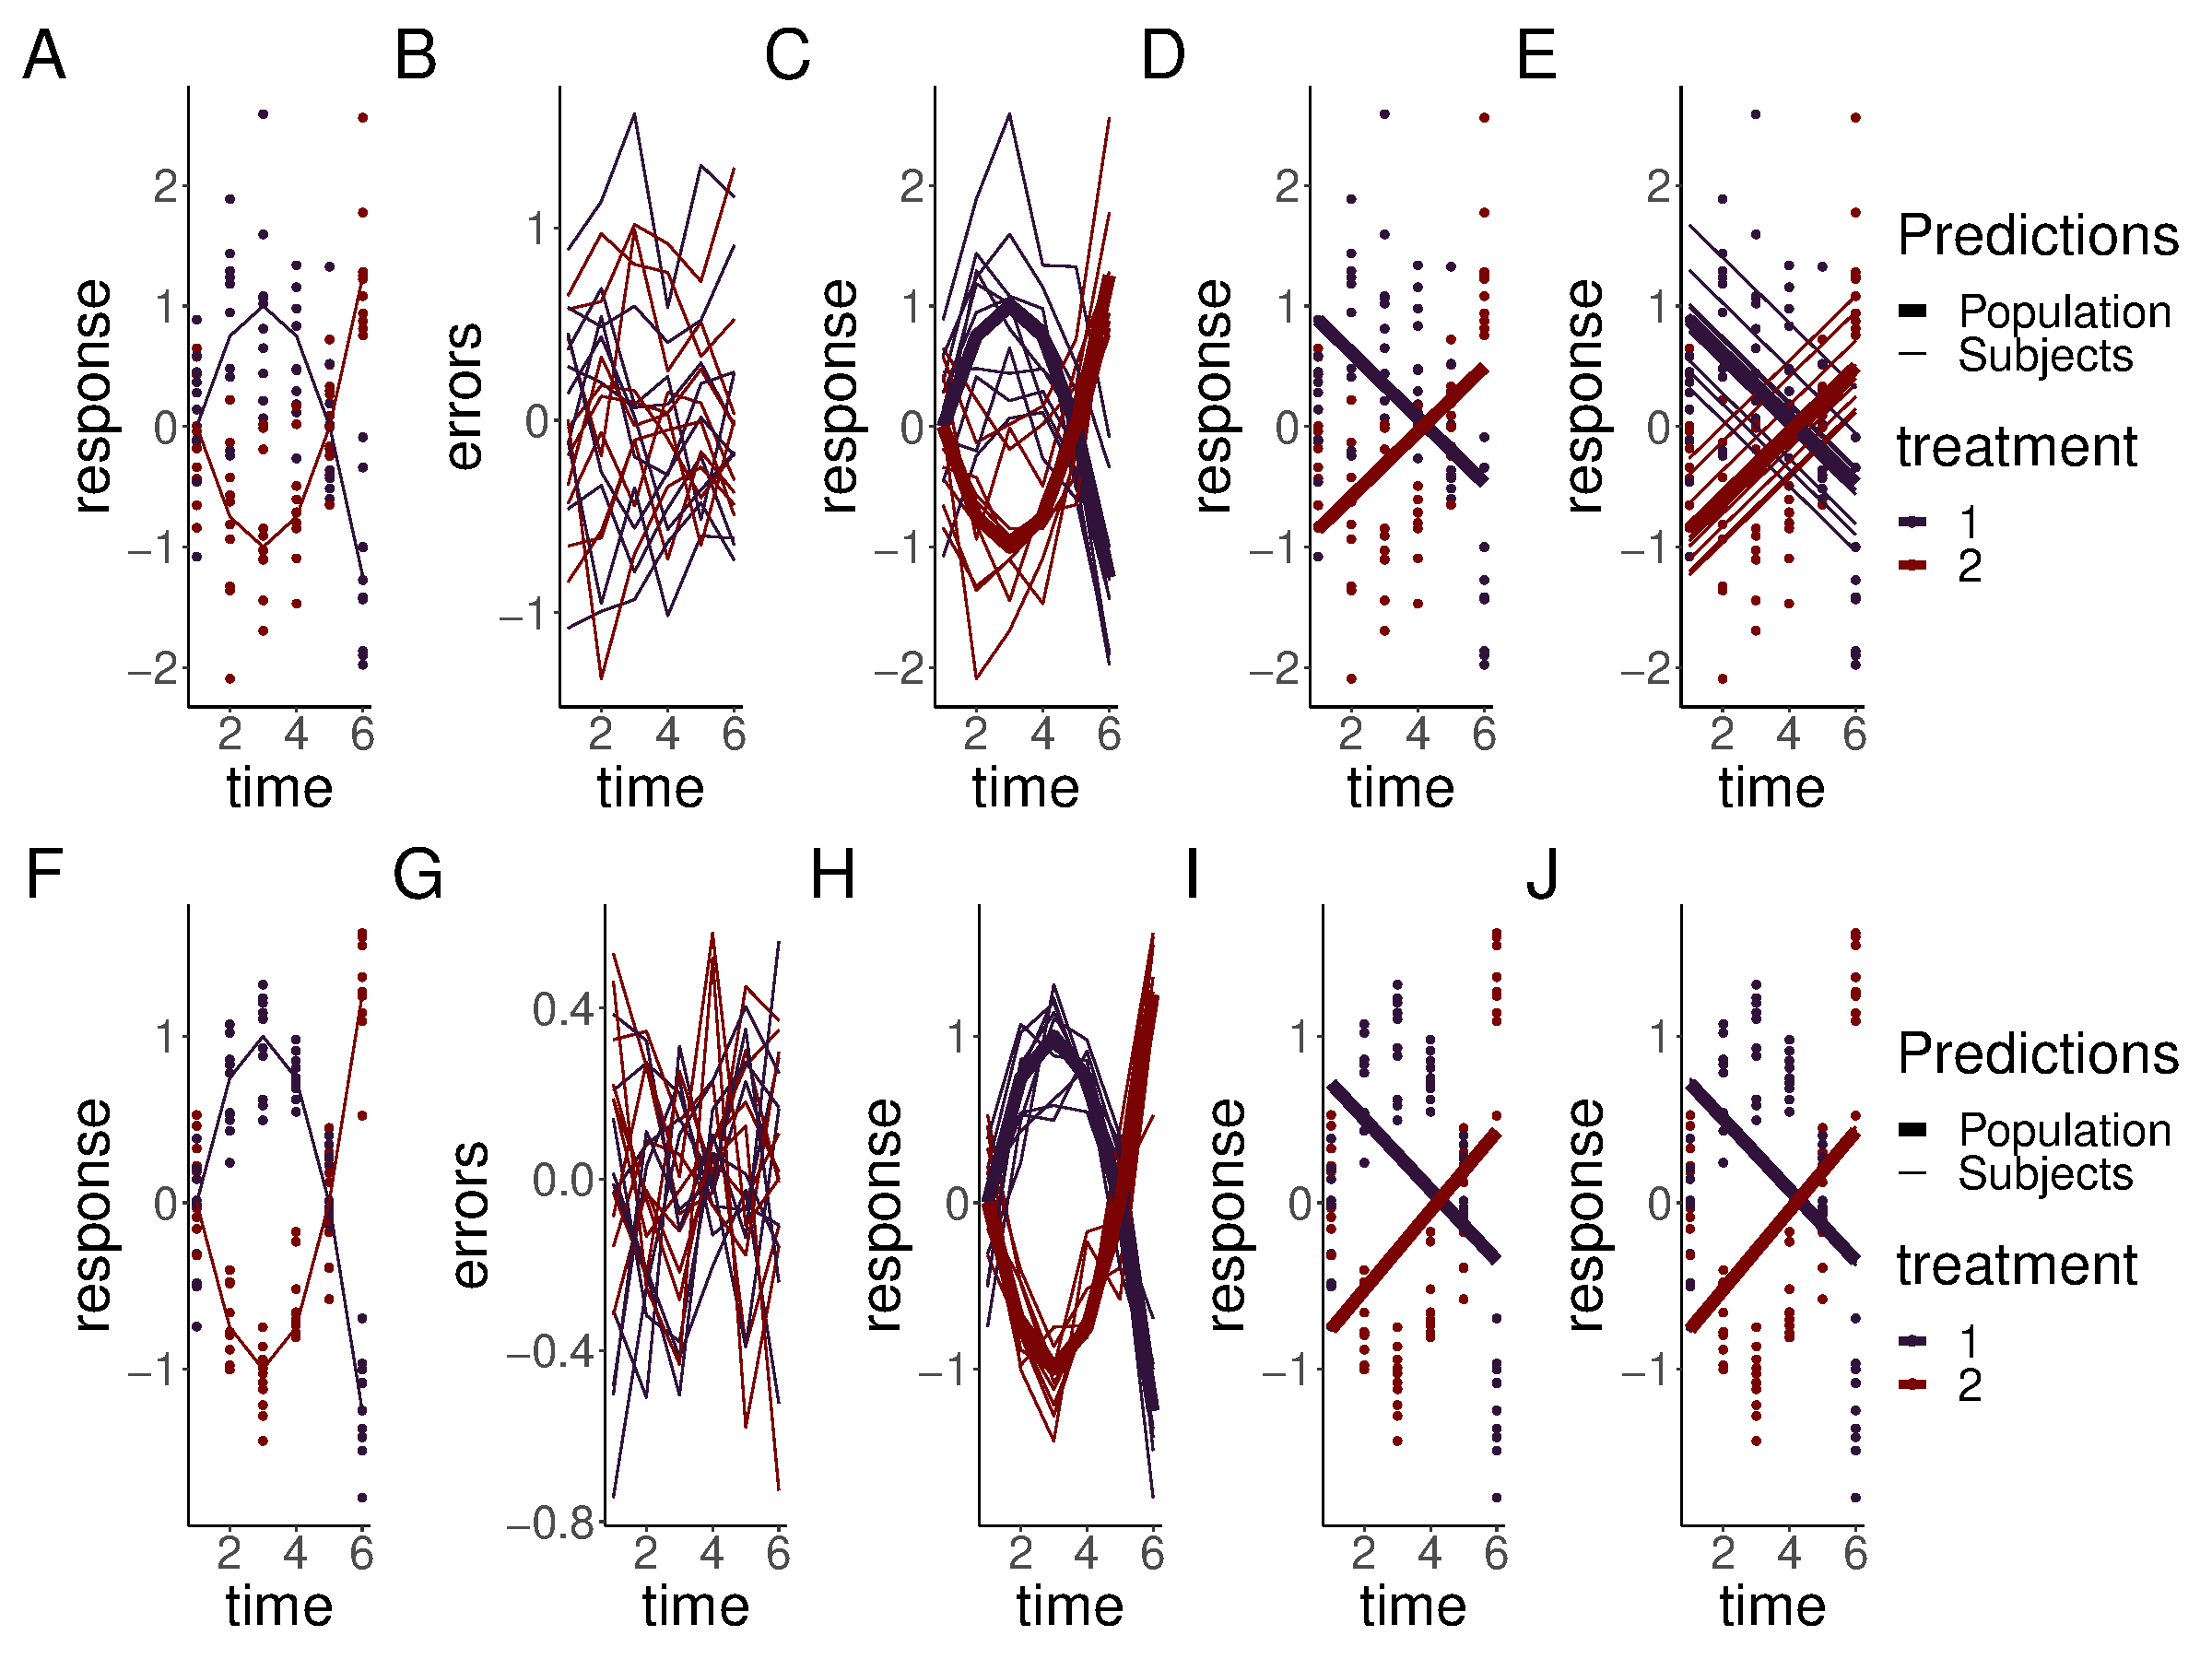
\includegraphics{00-Full_document_files/figure-latex/quadratic-cases-Appendix-1} \caption{Simulated quadratic responses from two groups with correlated (top row) or independent (bottom row) errors using a rm-ANOVA model and a LMEM. A, F:Simulated data with known mean response and individual responses (points) showing the dispersion of the data. B,G: Generated errors showing the difference in the behavior of correlated and independent errors. C,H: Simulated data with thin lines representing individual trajectories. D,I: Estimations from the rm-ANOVA model for the mean group response. E, J: Estimations from the LMEM for the mean group response and individual responses (thin lines). In all panels, thick lines are the predicted mean response per group, thin lines are the random effects for each subject and points represent the original raw data. Both rm-ANOVA and the LMEM are not able to capture the changes in each group over time.}\label{fig:quadratic-cases-Appendix}
\end{figure}

\hypertarget{basis-functions-and-gams}{%
\subsection{Basis functions and GAMs}\label{basis-functions-and-gams}}

This code produces Figure \ref{fig:basis-plot} from the main manuscript. Briefly, a non-linear (quadratic) response is simulated a gam model is fitted and the basis are extracted in order to explain how the smooth is constructed. The code for data simulation is used again here for the sake of keeping the same structure, although the data can be simulated in a more simple fashion.

\begin{lstlisting}[language=R]
#generate the response: the same initial procedure from the previous section to simulate
#the response
set.seed(1)
n_time = 6
 x <- seq(1,6, length.out = n_time)
 mu <- matrix(0, length(x), 2)
 mu[, 1] <-  -(0.25 * x^2) +1.5*x-1.25 #mean response
 mu[, 2] <- (0.25 * x^2) -1.5*x+1.25 #mean response
 y <- array(0, dim = c(length(x), 2, 10))
 errors <- array(0, dim = c(length(x), 2, 10))
 for (i in 1:2) {     # number of treatments
     for (j in 1:10) {  # number of subjects
         # compound symmetry errors
         errors[, i, j] <- rmvn(1, rep(0, length(x)), 0.1 * diag(6) + 0.25 * matrix(1, 6, 6))
         y[, i, j] <- mu[, i] + errors[, i, j]
     }
 }
 
 #label each table
  dimnames(y) <- list(time = x, treatment = 1:2, subject = 1:10)
 dimnames(errors) <- list(time = x, treatment = 1:2, subject = 1:10)
 dimnames(mu) <- list(time = x, treatment = 1:2)
 
 #Convert to dataframes with subject, time and group columns
 dat <- as.data.frame.table(y, responseName = "y")
 dat_errors <- as.data.frame.table(errors, responseName = "errors")
 dat_mu <- as.data.frame.table(mu, responseName = "mu")
 dat <- left_join(dat, dat_errors, by = c("time", "treatment", "subject"))
 dat <- left_join(dat, dat_mu, by = c("time", "treatment"))
 dat$time <- as.numeric(as.character(dat$time))
 
 #label subject per group
 dat <- dat %>%
     mutate(subject = factor(paste(subject, treatment, sep = "-")))
  
 #extract  "Group 1" to fit the GAM
  dat<-subset(dat,treatment==1)
 #keep just the response and timepoint columns
   dat<-dat[,c('y','time')]

   #GAM model of time, 5 knots
gm<-gam(y~s(time,k=5),data=dat)

#model_matrix (also known as) 'design matrix'
#will contain the smooths used to create  model 'gm'
model_matrix<-as.data.frame(predict(gm,type='lpmatrix'))


time<-c(1:6)

basis<-model_matrix[1:6,] #extracting basis (because the values are repeated after every 6 rows)
#basis<-model_matrix[1:6,-1] #extracting basis
colnames(basis)[colnames(basis)=="(Intercept)"]<-"s(time).0"
basis<-basis %>% #pivoting to long format
  pivot_longer(
    cols=starts_with("s")
  )%>%
  arrange(name) #ordering

#length of dataframe to be created: number of knots by number of timepoints (minus 1 for the intercept that we won't plot)
ln<-6*(length(coef(gm))) 

basis_plot<-data.frame(Basis=integer(ln),
                       value_orig=double(ln),
                       time=integer(ln),
                       cof=double(ln)
)

basis_plot$time<-rep(time) #pasting timepoints
basis_plot$Basis<-factor(rep(c(1:5),each=6)) #pasting basis number values
basis_plot$value_orig<-basis$value #pasting basis values
basis_plot$cof<-rep(coef(gm)[1:5],each=6) #pasting coefficients
basis_plot<-basis_plot%>%
  mutate(mod_val=value_orig*cof) #the create the predicted values the bases need to be 
#multiplied by the coefficients

#creating labeller to change the labels in the basis plots

basis_names<-c(
  `1`="Intercept",
  `2`="1",
  `3`="2",
  `4`="3",
  `5`="4"
)

#calculating the final smooth by aggregating the basis functions

smooth<-basis_plot%>% 
  group_by(time)%>%
  summarize(smooth=sum(mod_val))


#original basis
sz<-1
p11<-ggplot(basis_plot,
            aes(x=time,
                y=value_orig,
                colour=as.factor(Basis)
                )
            )+
  geom_line(size=sz,
            show.legend=FALSE)+
  geom_point(size=sz+1,
             show.legend = FALSE)+
  labs(y='Basis functions')+
  facet_wrap(~Basis,
             labeller = as_labeller(basis_names)
             )+
  theme_classic()+
  thm
  

#penalized basis
p12<-ggplot(basis_plot,
            aes(x=time,
                y=mod_val,
                colour=as.factor(Basis)
                )
            )+
  geom_line(show.legend = FALSE,
            size=sz)+
  geom_point(show.legend = FALSE,
             size=sz+1)+
  labs(y='Penalized \n basis functions')+
  scale_y_continuous(breaks=seq(-1,1,1))+
  facet_wrap(~Basis,
             labeller=as_labeller(basis_names)
             )+
  theme_classic()+
  thm

#heatmap of the coefficients
x_labels<-c("Intercept","1","2","3","4")
p13<-ggplot(basis_plot,
            aes(x=Basis,
                y=Basis))+
  geom_tile(aes(fill = cof), 
            colour = "black") +
    scale_fill_gradient(low = "white",
                        high = "#B50A2AFF")+ #color picked from KikiMedium
  labs(x='Basis',
       y='Basis')+
  scale_x_discrete(labels=x_labels)+
  geom_text(aes(label=round(cof,2)),
            size=7,
            show.legend = FALSE)+
  theme_classic()+
  theme(legend.title = element_blank())
  
#plotting simulated datapoints and smooth term
p14<-ggplot(data=dat,
            aes(x=time,y=y))+
  geom_point(size=sz+1)+
  labs(y='Simulated \n response')+
  geom_line(data=smooth,
            aes(x=time,
                y=smooth),
            color="#6C581DFF",
            size=sz+1)+
  theme_classic()
  

#Combining all
b_plot<-p11+p13+p12+p14+plot_annotation(tag_levels='A')&
  theme(
     text=element_text(size=18)
     )
\end{lstlisting}

\begin{figure}[H]

{\centering 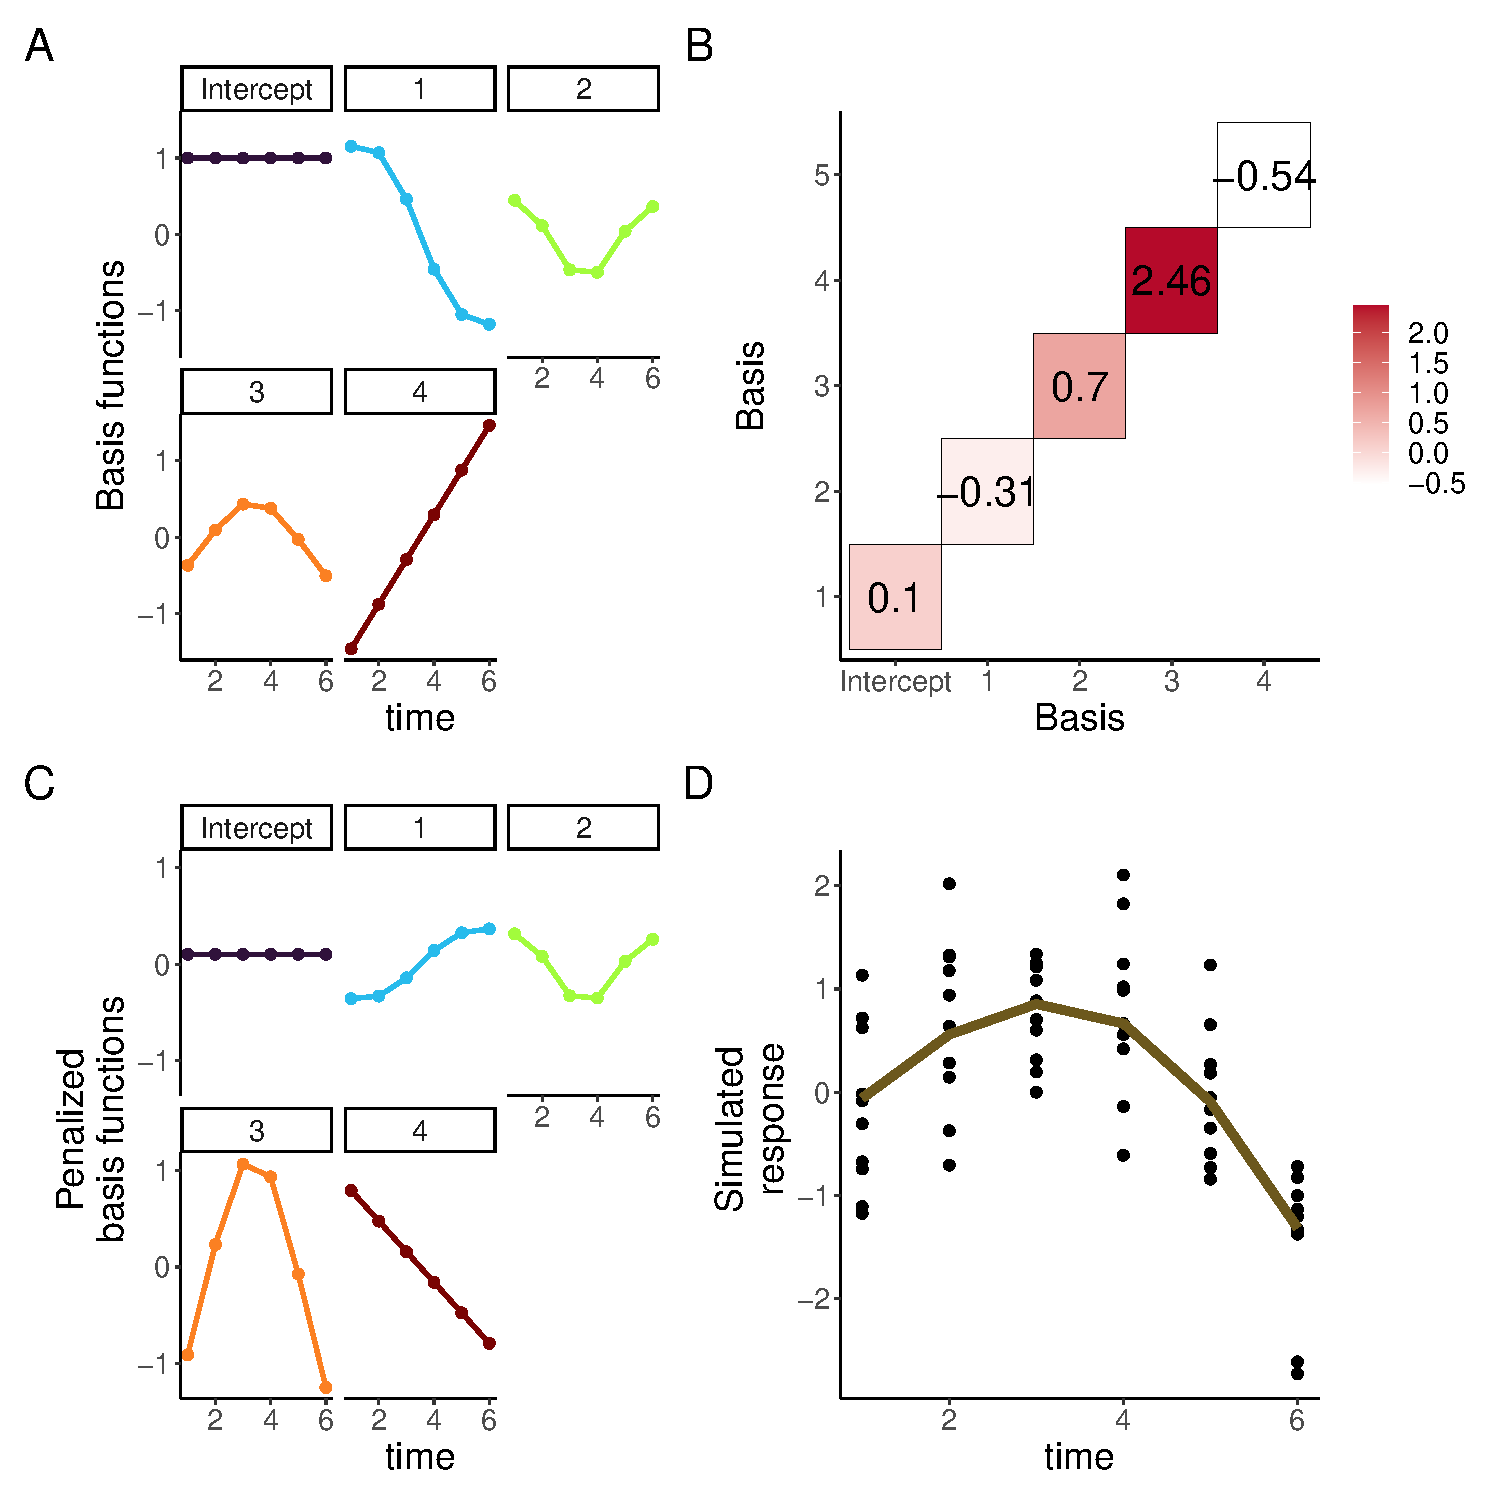
\includegraphics[width=0.75\linewidth,]{00-Full_document_files/figure-latex/basis-plot-appendix-1} 

}

\caption{Basis functions for a single smoother for time with five knots. A: Basis functions for a single smoother for time for the simulated data of Group 1 from Figure 2. B: Matrix of basis function weights. Each basis function is multiplied by a coefficient which can be positive or negative. The coefficient determines the overall effect of each basis in the final smoother. C: Weighted basis functions. Each of the four basis functions of panel A has been weighted by the corresponding coefficient shown in Panel B. Note the corresponding increase (or decrease) in magnitude of each weighted basis function. D: Smoother for time and original data points. The smoother (line) is the result of the sum of each weighted basis function at each time point, with simulated values for the group shown as points.}\label{fig:basis-plot-appendix}
\end{figure}

\hypertarget{tumor-data-simulation}{%
\section{Longitudinal biomedical data simulation and GAMs}\label{tumor-data-simulation}}

This section describes how to fit GAMs to longitudinal data using simulated data. First, data is simulated according to Section \ref{longitudinal-GAMs}, where reported data of oxygen saturation (\(\mbox{StO}_2\)) in tumors under either chemotherapy or saline control is used as a starting point to generate individual responses in each group.

\begin{lstlisting}[language=R]
set.seed(1)
#Dataframe that contains the original reported trends
dat<-tibble(StO2=c(4,27,3,2,0.5,7,4,50,45,56),
            Day=rep(c(0,2,5,7,10),times=2),
            Group=as.factor(rep(c("Control","Treatment"),each=5))
            )


## plot the mean response
f1<-ggplot(dat, 
           aes(x = Day, 
               y = StO2, 
               color = Group)) +
    geom_line(size=1,
              show.legend = FALSE)+
    geom_point(show.legend = FALSE,
               size=1.5,
               alpha=0.5)+
  labs(y=expression(paste(StO[2],
                          ' (real)')))+
  theme_classic()+
  thm+
    scale_x_continuous(breaks=c(0,5,10))+
    scale_y_continuous(breaks=c(0,40))+
  plot_layout(tag_level = 'new')+
  theme(
    plot.background = element_rect(fill = "transparent", 
                                   color = NA),
    axis.text=element_text(size=14)
  )


#This function simulates data for the tumor data using default parameters of 10 observations per time point,and Standard deviation (sd) of 5%.
#Because physiologically StO2 cannot go below 0%, data is  generated with a cutoff value of 0.0001 (the "StO2_sim")

simulate_data <- function(dat, n = 10, sd = 5) {
    dat_sim <- dat %>%
        slice(rep(1:n(), each = n)) %>%
        group_by(Group, Day) %>%
        mutate(
               StO2_sim = pmax(rnorm(n, StO2, sd), 0.0001),
               subject=rep(1:10),
               subject=factor(paste(subject, Group, sep = "-"))
               ) %>%
        ungroup()

    return(dat_sim)
}


#subject = factor(paste(subject, treatment, sep = "-")))
n <- 10 #number of observations
sd <- 10 #approximate sd from paper
df <- 6
dat_sim <- simulate_data(dat, n, sd)

#plotting simulated data
f2<-ggplot(dat_sim, 
           aes(x = Day, 
               y = StO2_sim, 
               color = Group)) +
    geom_point(show.legend=FALSE,
               size=1.5,
               alpha=0.5)+
    stat_summary(aes(y = StO2_sim,
                     group=Group), 
                 fun=mean, geom="line",
                 size=1,
                 show.legend = FALSE)+
  labs(y=expression(atop(StO[2],
                         '(simulated)')))+
  theme_classic()+
  theme(
    axis.text=element_text(size=22)
  )+
  thm+
    scale_x_continuous(breaks=c(0,2,5,7,10))
\end{lstlisting}

\hypertarget{workflow}{%
\subsection{A basic Workflow for GAMs}\label{workflow}}

This section shows a basic workflow to fit a series of increasingly complex GAMs to the simulated data from the previous section. Graphical and parameter diagnostics for goodness of fit are discussed, as well as model comparison via AIC (Aikake Information Criterion).

\hypertarget{first-model}{%
\subsubsection{First model}\label{first-model}}

The first model fitted to the data is one that only accounts for different smooths by day. The model syntax specifies that \passthrough{\lstinline!gam\_00!} is the object that will contain all the model information, and that the model attempts to explain changes in \passthrough{\lstinline!StO2\_sim!} (simulated \(\mbox{StO}_2\)) using a smooth per \passthrough{\lstinline!Day!}. The model will use 5 knots (\passthrough{\lstinline!k=5!}) for the smooth. The smooth is constructed by default using thin plate regression splines. The smoothing parameter estimation method used is the restricted maximum likelihood (\passthrough{\lstinline!REML!}).

\begin{lstlisting}[language=R]
gam_00<-gam(StO2_sim ~ s(Day, k = 5),
            method='REML',
            data  = dat_sim)
\end{lstlisting}

To obtain model diagnostics, two methodologies are to be used: 1) graphical diagnostics, and 2) a model check. In the first case, the functions \passthrough{\lstinline!appraise!} and \passthrough{\lstinline!draw!} from the package \emph{gratia} can be used to obtain a single output with all the graphical diagnostics. For model check, the functions \passthrough{\lstinline!gam.check!} and \passthrough{\lstinline!summary!} from \emph{mgcv} provide detailed information about the model fit and its parameters.



\hypertarget{graphical-diagnostics}{%
\paragraph{Graphical diagnostics}\label{graphical-diagnostics}}

\begin{figure}[H]

{\centering 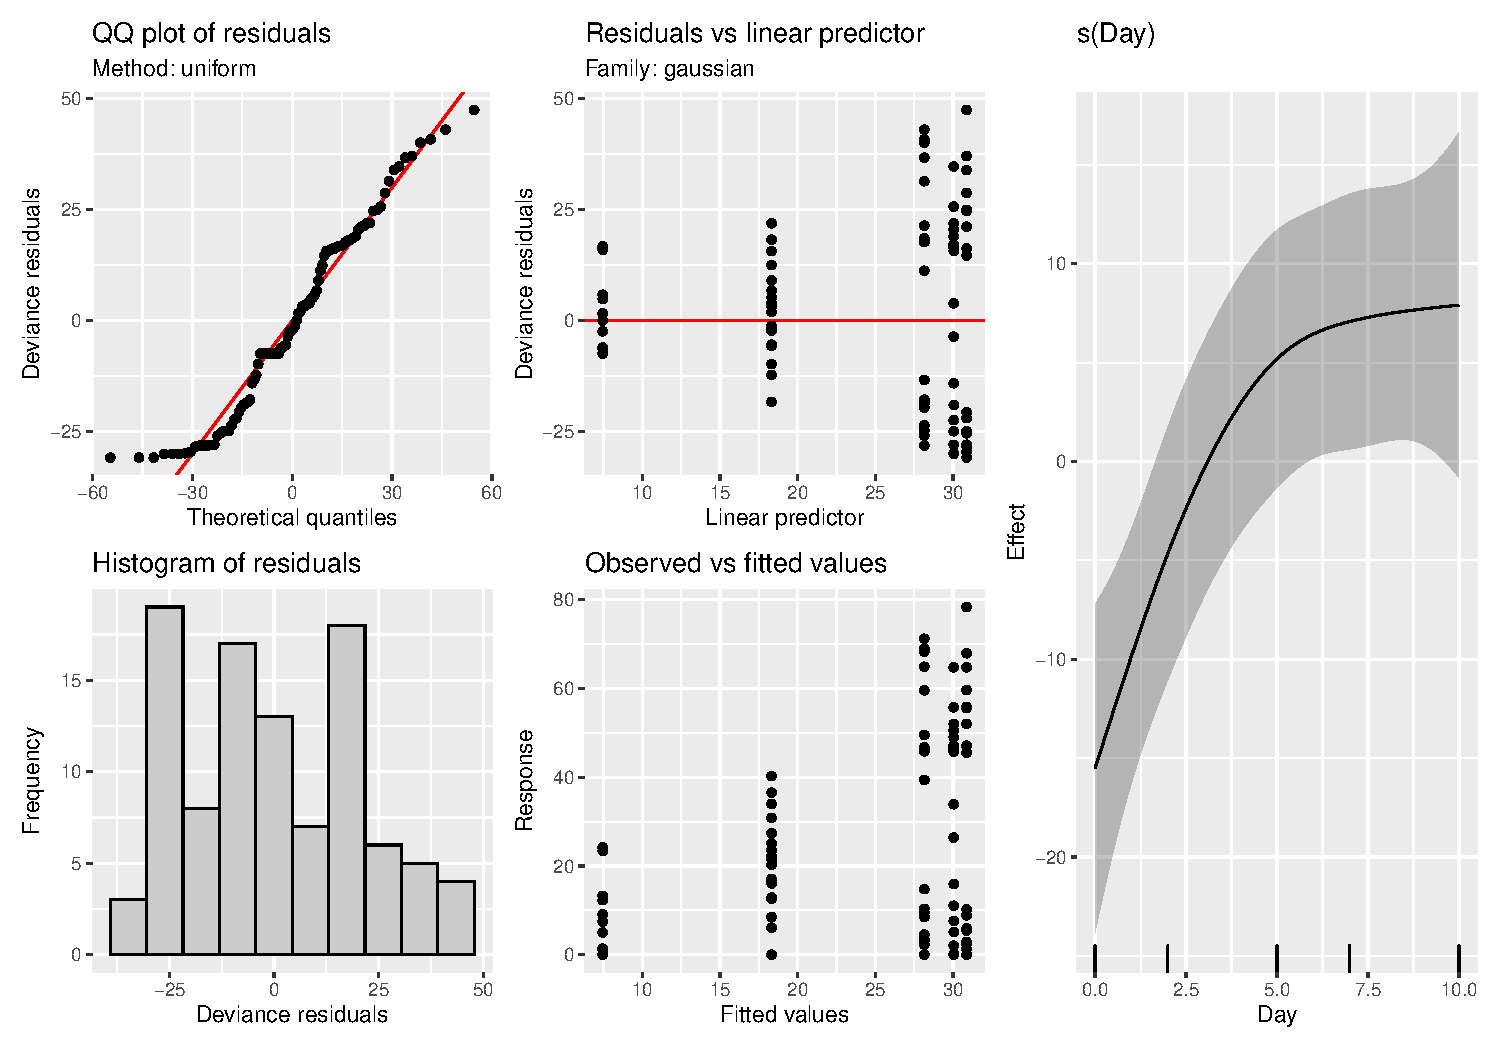
\includegraphics[width=0.75\linewidth,]{00-Full_document_files/figure-latex/first-GAM-diag-1} 

}

\caption{Graphical diagnostics for the first GAM model. Left: Graphical diagnostics provided by the function \passthrough{\lstinline!appraise!} from the package \emph{gratia}. Right: Fitted smooth for the model, provided by the function \passthrough{\lstinline!draw!}.}\label{fig:first-GAM-diag}
\end{figure}

From the output of the function \passthrough{\lstinline!appraise!} in Figure \ref{fig:first-GAM-diag}, the major indicators of concern about the model are the QQ plot of residuals and the histogram of residuals. The QQ plot shows that the errors are not reasonably located along the 45\(^{\circ}\) line (which indicates normality), as there are multiple points that deviate from the trend, specially in the tails. The histogram also shows that the variation (residuals) is not following the assumption of a normal distribution.

The \passthrough{\lstinline!draw!} function permits to plot the smooths as \passthrough{\lstinline!ggplot2!} objects, which eases subsequent manipulation, if desired. Because model \passthrough{\lstinline!gam\_00!} specifies only one smooth for the time covariate (Day), the plot only contains only one smooth. Note that the smooth shows an almost linear profile.

\hypertarget{model-check}{%
\paragraph{Model check}\label{model-check}}

\begin{lstlisting}[language=R]
#need to add figure number and caption
gam.check(gam_00)
\end{lstlisting}

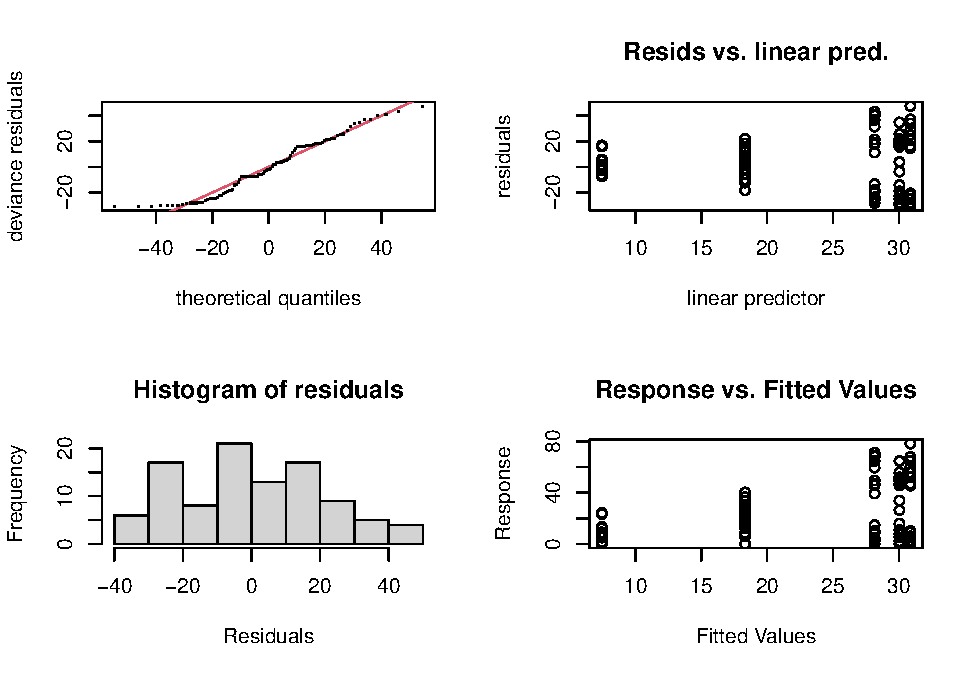
\includegraphics{00-Full_document_files/figure-latex/first-GAM-check-1}

\begin{lstlisting}
## 
## Method: REML   Optimizer: outer newton
## full convergence after 5 iterations.
## Gradient range [-0.0003727881,-6.621452e-07]
## (score 444.0118 & scale 450.6638).
## Hessian positive definite, eigenvalue range [0.3881695,49.00676].
## Model rank =  5 / 5 
## 
## Basis dimension (k) checking results. Low p-value (k-index<1) may
## indicate that k is too low, especially if edf is close to k'.
## 
##          k'  edf k-index p-value    
## s(Day) 4.00 2.11    0.36  <2e-16 ***
## ---
## Signif. codes:  0 '***' 0.001 '**' 0.01 '*' 0.05 '.' 0.1 ' ' 1
\end{lstlisting}

\begin{lstlisting}[language=R]
summary(gam_00)
\end{lstlisting}

\begin{lstlisting}
## 
## Family: gaussian 
## Link function: identity 
## 
## Formula:
## StO2_sim ~ s(Day, k = 5)
## 
## Parametric coefficients:
##             Estimate Std. Error t value Pr(>|t|)    
## (Intercept)   22.967      2.123   10.82   <2e-16 ***
## ---
## Signif. codes:  0 '***' 0.001 '**' 0.01 '*' 0.05 '.' 0.1 ' ' 1
## 
## Approximate significance of smooth terms:
##          edf Ref.df     F  p-value    
## s(Day) 2.114  2.565 7.633 0.000517 ***
## ---
## Signif. codes:  0 '***' 0.001 '**' 0.01 '*' 0.05 '.' 0.1 ' ' 1
## 
## R-sq.(adj) =  0.153   Deviance explained = 17.2%
## -REML = 444.01  Scale est. = 450.66    n = 100
\end{lstlisting}

Special attention must be paid to the `k-index' from \passthrough{\lstinline!gam.check!}. This parameter indicates if the basis dimension of the smooth is adequate, i.e., it checks that the basis used to create the smooth are adequate to capture the trends in the data. If the model is not adequately capturing the trens in the data, this is indicated by a low k-index value (\textless1). From the output, it can be seen that the k-index is 0.36, which indicates that the model is not capturing the variability in the data. The \passthrough{\lstinline!edf!} (effective degrees of freedom) is an indicator of the complexity of the smooth. Here the complexity of the smooth is comparable to that of a 4th degree polynomial.

From the \passthrough{\lstinline!summary!} function, information about the assumed distribution of the errors (Gaussian in this case) and the link function can be obtained. The link function is `identity' as the model does not make any transformation on the predictors. The `significance of smooth terms' \emph{p-value} indicates if each smooth is adding significance to the model. Here, the \emph{p-value} is low but we have seen that there are issues with the model from the previous outputs. Finally, the `deviance explained' indicates how much of the data the model is able to capture, which in this case corresponds to \(\approx\) 17\%.

\hypertarget{second-model}{%
\subsubsection{Second model}\label{second-model}}

The major flaw of \passthrough{\lstinline!gam\_00!} is that this model is not taking into account the fact that the data is nested in groups. The next iteration is a model where a different smooth of time (Day) is assigned for each group using \passthrough{\lstinline!by=Group!} in the model syntax.

\begin{lstlisting}[language=R]
gam_01<-gam(StO2_sim ~ s(Day, by=Group,k = 5),
            method='REML',
            data  = dat_sim)

gam.check(gam_01)
\end{lstlisting}

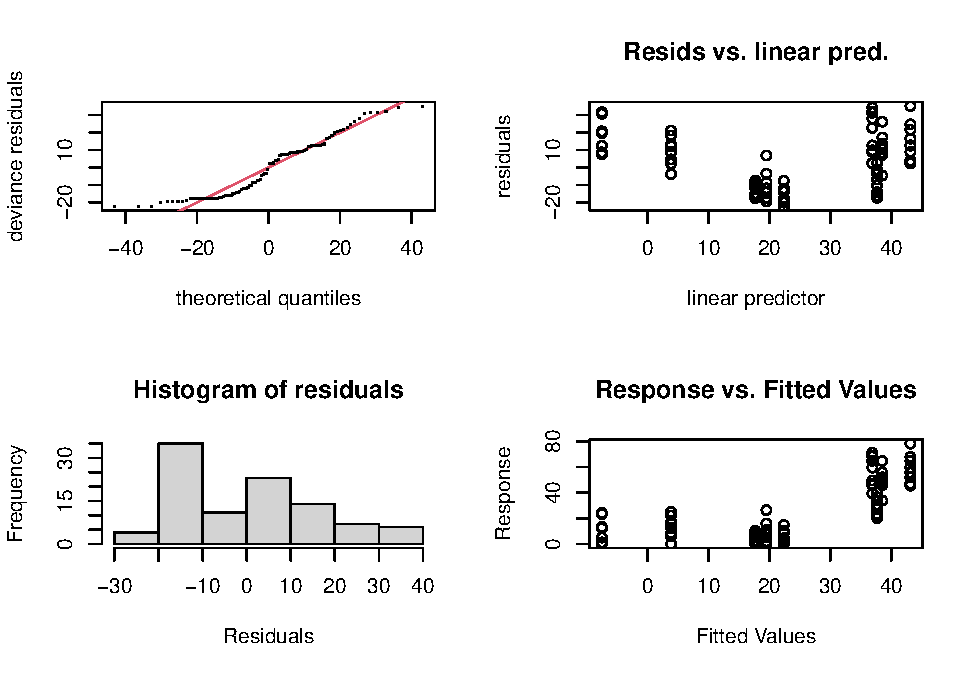
\includegraphics{00-Full_document_files/figure-latex/second-GAM-1}

\begin{lstlisting}
## 
## Method: REML   Optimizer: outer newton
## full convergence after 7 iterations.
## Gradient range [-5.51754e-05,2.671715e-06]
## (score 423.3916 & scale 280.8777).
## Hessian positive definite, eigenvalue range [0.3162258,48.5557].
## Model rank =  9 / 9 
## 
## Basis dimension (k) checking results. Low p-value (k-index<1) may
## indicate that k is too low, especially if edf is close to k'.
## 
##                         k'  edf k-index p-value    
## s(Day):GroupControl   4.00 3.39    0.43  <2e-16 ***
## s(Day):GroupTreatment 4.00 3.23    0.43  <2e-16 ***
## ---
## Signif. codes:  0 '***' 0.001 '**' 0.01 '*' 0.05 '.' 0.1 ' ' 1
\end{lstlisting}

\begin{lstlisting}[language=R]
summary(gam_01)
\end{lstlisting}

\begin{lstlisting}
## 
## Family: gaussian 
## Link function: identity 
## 
## Formula:
## StO2_sim ~ s(Day, by = Group, k = 5)
## 
## Parametric coefficients:
##             Estimate Std. Error t value Pr(>|t|)    
## (Intercept)   22.967      1.676    13.7   <2e-16 ***
## ---
## Signif. codes:  0 '***' 0.001 '**' 0.01 '*' 0.05 '.' 0.1 ' ' 1
## 
## Approximate significance of smooth terms:
##                         edf Ref.df      F p-value    
## s(Day):GroupControl   3.392  3.794  3.817  0.0304 *  
## s(Day):GroupTreatment 3.229  3.682 21.174  <2e-16 ***
## ---
## Signif. codes:  0 '***' 0.001 '**' 0.01 '*' 0.05 '.' 0.1 ' ' 1
## 
## R-sq.(adj) =  0.472   Deviance explained = 50.8%
## -REML = 423.39  Scale est. = 280.88    n = 100
\end{lstlisting}

Diagnostics for this model indicate that the k-index is still below 1 (0.43 from \passthrough{\lstinline!gam.check!}), and that the residuals are still not following a normal distribution (Figure \ref{fig:second-GAM-diag}). Moreover, the smooths (plotted via the \passthrough{\lstinline!draw()!} function) appear with a fairly linear profile, which indicates they are still not capturing the trends observed in the data. From \passthrough{\lstinline!summary()!}, the deviance explained by the model is \(\approx\) 51\%.



\begin{figure}[H]

{\centering 
\includegraphics[width=0.75\linewidth,]{00-Full_document_files/figure-latex/second-GAM-diag-1} 

}

\caption{Graphical diagnostics for the second GAM model. Left: Graphical diagnostics provided by the function \passthrough{\lstinline!appraise!} from the package \emph{gratia}. Right: Fitted smooth for the model, provided by the function \passthrough{\lstinline!draw!}.}\label{fig:second-GAM-diag}
\end{figure}

\hypertarget{third-model}{%
\subsubsection{Third model}\label{third-model}}

Model \passthrough{\lstinline!gam\_00!} was built for didactic purposes to cover the simplest case, but it does not account for the nesting of the data by Group, which is apparent from the type of smooth fitted, the model diagnostics, and, the low variance explained by the model. On the other hand, \passthrough{\lstinline!gam\_01!} takes into account the nesting within each group and provides better variance explanation, but as indicated in Section \ref{longitudinal-GAMs}, in order to differentiate between each group a parametric term needs to be added to the model for the interaction of \emph{Day} and \emph{Group}.

\begin{lstlisting}[language=R]
#GAM for StO2

m1 <- gam(StO2_sim ~ Group+s(Day, by = Group, k = 5),
            method='REML',
            data  = dat_sim)

gam.check(m1)
\end{lstlisting}

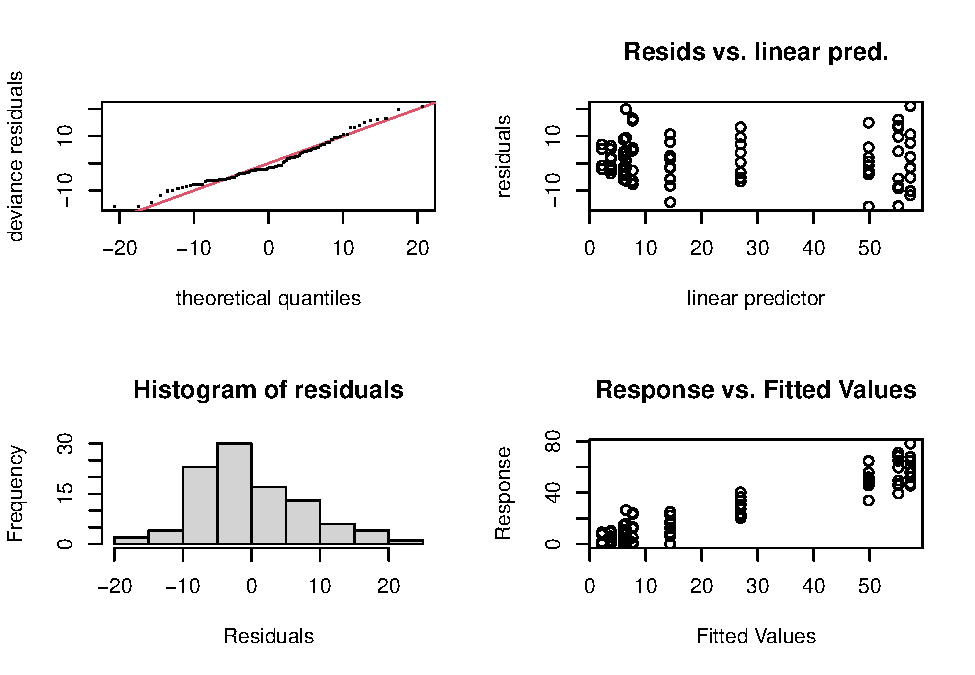
\includegraphics{00-Full_document_files/figure-latex/final-model-Appendix-1}

\begin{lstlisting}
## 
## Method: REML   Optimizer: outer newton
## full convergence after 10 iterations.
## Gradient range [-8.164307e-08,1.500338e-08]
## (score 355.8554 & scale 64.53344).
## Hessian positive definite, eigenvalue range [1.174841,48.08834].
## Model rank =  10 / 10 
## 
## Basis dimension (k) checking results. Low p-value (k-index<1) may
## indicate that k is too low, especially if edf is close to k'.
## 
##                         k'  edf k-index p-value
## s(Day):GroupControl   4.00 3.87    1.02    0.59
## s(Day):GroupTreatment 4.00 3.88    1.02    0.54
\end{lstlisting}

\begin{lstlisting}[language=R]
summary(m1)
\end{lstlisting}

\begin{lstlisting}
## 
## Family: gaussian 
## Link function: identity 
## 
## Formula:
## StO2_sim ~ Group + s(Day, by = Group, k = 5)
## 
## Parametric coefficients:
##                Estimate Std. Error t value Pr(>|t|)    
## (Intercept)       9.084      1.136   7.996 4.09e-12 ***
## GroupTreatment   27.766      1.607  17.282  < 2e-16 ***
## ---
## Signif. codes:  0 '***' 0.001 '**' 0.01 '*' 0.05 '.' 0.1 ' ' 1
## 
## Approximate significance of smooth terms:
##                         edf Ref.df     F p-value    
## s(Day):GroupControl   3.873  3.990 17.57  <2e-16 ***
## s(Day):GroupTreatment 3.879  3.991 89.33  <2e-16 ***
## ---
## Signif. codes:  0 '***' 0.001 '**' 0.01 '*' 0.05 '.' 0.1 ' ' 1
## 
## R-sq.(adj) =  0.879   Deviance explained = 88.9%
## -REML = 355.86  Scale est. = 64.533    n = 100
\end{lstlisting}

The resulting model is \passthrough{\lstinline!m1!}, which is the model fitted in the main manuscript. By using \passthrough{\lstinline!appraise()!} and \passthrough{\lstinline!draw!} on this model (Figure \ref{fig:final-GAM-diag}) we see that the trend on the QQ plot has improved, the histogram of the residuals appears to be reasonably distributed, and the smooths are capturing the trend of the data within each group. From \passthrough{\lstinline!gam.check!}, the k-index is now at an acceptable value (\(\approx\) 1.02), and \passthrough{\lstinline!summary!} now indicates that the model is able to capture 89\% of the variance in the data.



\begin{figure}[H]

{\centering 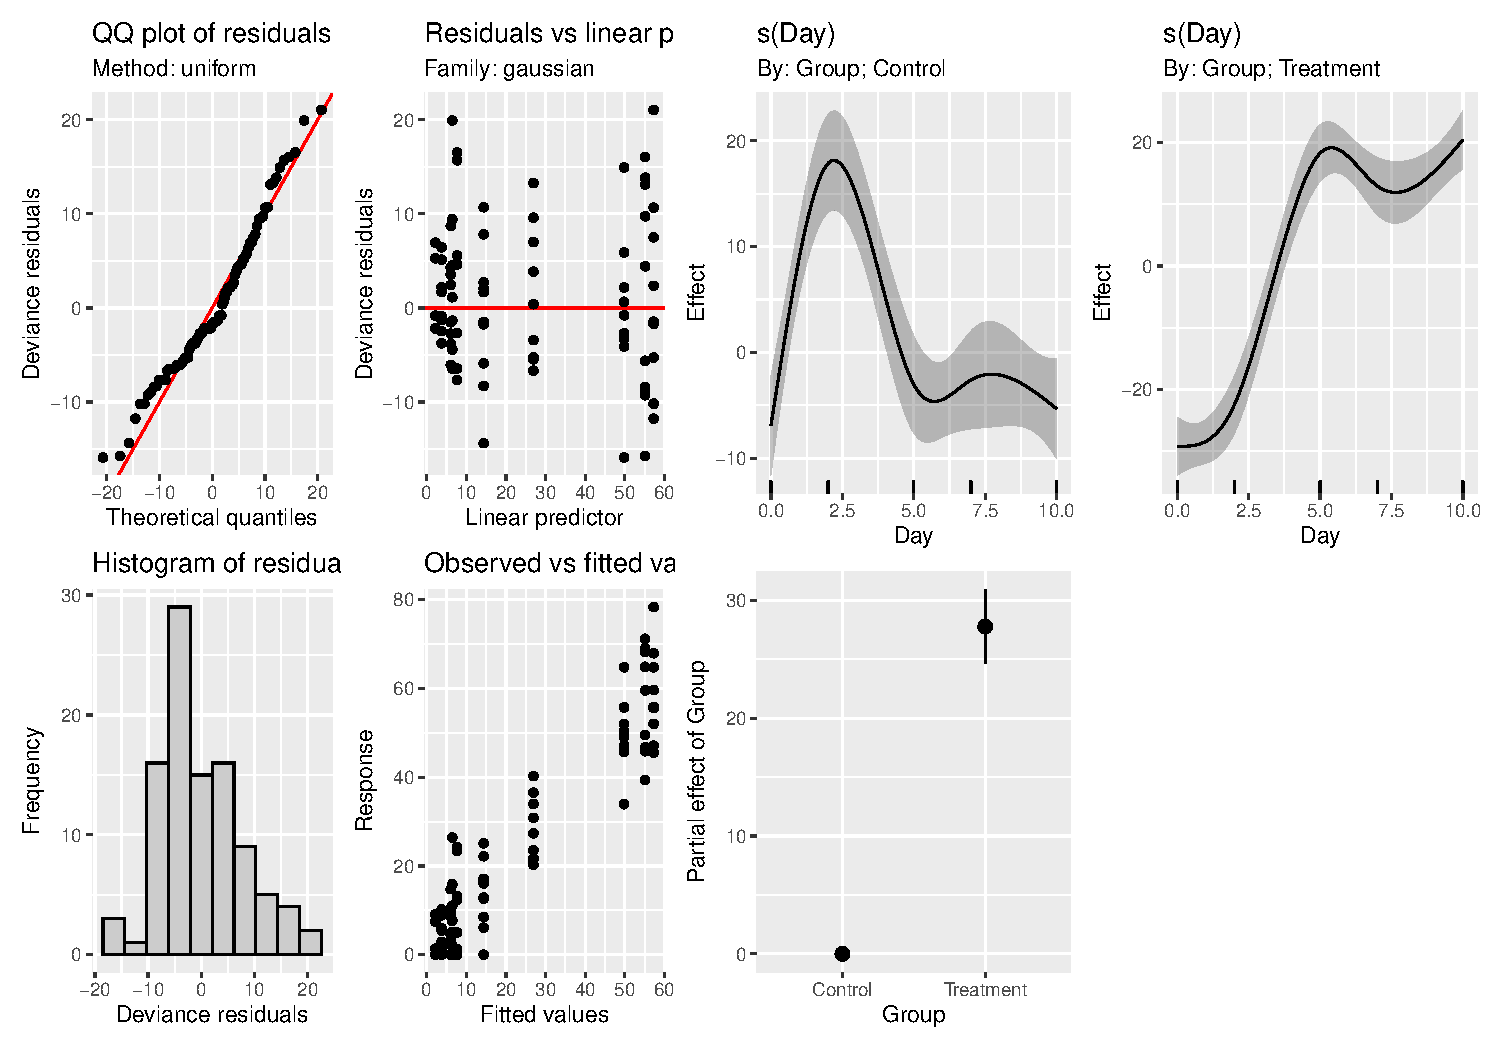
\includegraphics[width=0.75\linewidth,]{00-Full_document_files/figure-latex/final-GAM-diag-1} 

}

\caption{Graphical diagnostics for the final GAM model. Left: Graphical diagnostics provided by the function \passthrough{\lstinline!appraise!} from the package \emph{gratia}. Right: Fitted smooths for the model, provided by the function \passthrough{\lstinline!draw!}.}\label{fig:final-GAM-diag}
\end{figure}

\hypertarget{comparing-models-via-aic}{%
\subsubsection{Comparing models via AIC}\label{comparing-models-via-aic}}

One final comparison that can be made for model selection involves the use of the Aikake Information Criterion (AIC). This metric is used to estimate information loss, which we want to minimize with an appropriate model. Therefore, when 2 or more models are compared, the model with lower AIC is preferred. In R, the comparison is done using the \passthrough{\lstinline!AIC!} function.

\begin{lstlisting}[language=R]
AIC(gam_00,gam_01,m1)
\end{lstlisting}

\begin{lstlisting}
##               df      AIC
## gam_00  4.564893 900.8257
## gam_01  9.476137 858.6051
## m1     10.980983 712.2067
\end{lstlisting}

The output in this case is expected: model \passthrough{\lstinline!m1!} has a lower AIC (712.46) whereas the initial two models have higher AICs (900 and 858). The AIC should not be considered as the only estimator of model quality, instead to be used as complimentary information to the graphical diagnostics and model checks described above.

\hypertarget{pairwise-comparisons-of-smooth-confidence-intervals}{%
\paragraph{Pairwise comparisons of smooth confidence intervals}\label{pairwise-comparisons-of-smooth-confidence-intervals}}

The estimation of significant differences between each treatment group can be achieved via pairwise comparisons of the smooth confidence intervals as described in section \ref{GAM-significance}. In this case, the ``design matrix'' is used to estimate the pairwise comparisons (see main manuscript for details and associated references). Briefly, the ``design matrix'' (also known as the ``Xp matrix'') from the selected model (\passthrough{\lstinline!m1!}) is used to calculate a 95\% confidence interval of the difference between the smooth terms for each group. This approach allows to estimate the time intervals where a significant difference exists between the groups (confidence interval above or below 0). \textbf{All pairwise comparisons in this paper have been centered at the response scale to ease interpretation }.

\begin{lstlisting}[language=R]
##Pairwise comparisons
pdat <- expand.grid(Day = seq(0, 10, length = 400),
                    Group = c('Control', 'Treatment'))

##matrix that contains the basis functions evaluated at the points in pdat
    xp <- predict(m1, newdata = pdat, type = 'lpmatrix')

    
#Find columns in xp where the name contains "Control"
    c1 <- grepl('Control', colnames(xp))

#Find columns in xp where the name contains 'Treatment'
    c2 <- grepl('Treatment', colnames(xp))

#Find rows in pdat that correspond to either 'Control' or 'Treatment'
    r1 <- with(pdat, Group == 'Control')
    r2 <- with(pdat, Group == 'Treatment')

# In xp: find the rows that correspond to Control or Treatment, those that do not match will be
    #set to zero. Then, substract the values from the rows corresponding to 'Control' from those that correspond
    #to 'Treatment'
    X <- xp[r1, ] - xp[r2, ]

    ## remove columns that do not contain name 'Control' or 'Treatment'
    X[, ! (c1 | c2)] <- 0
    ## zero out the parametric cols, those that do not contain in the characters 's('
    #X[, !grepl('^s\\(', colnames(xp))] <- 0

    #Multiply matrix by model coefficients. X has (p,n) (rows, columns) and the coefficient matrix has
    #dimensions (n,1). The resulting matrix has dimensions (p,1)
    dif <- X %*% coef(m1)

    #comp<-test %*% coef(gam1)[3:10]

#Calculate standard error for the computed differences using the variance-covariance matrix
    #of the model
    se <- sqrt(rowSums((X %*% vcov(m1, unconditional = FALSE)) * X))
    crit <- qt(0.05/2, df.residual(m1), lower.tail = FALSE)
    #upper  limits
    upr <- dif + (crit * se)
    #lower limits
    lwr <- dif - (crit * se)
    #put all components in a dataframe for plotting
    comp1<-data.frame(pair = paste('Control', 'Treatment', sep = '-'),
               diff = dif,
               se = se,
               upper = upr,
               lower = lwr)



#add time point sequence
comp_StO2 <- cbind(Day = seq(0, 10, length = 400),
                   rbind(comp1))

#use function from the pairwise comparison plot in the manuscript to get the shaded regions
    
    my_list<-pairwise_limits(comp_StO2)
  rib_col<-'#EDD03AFF' #color for the ribbon
#plot the difference
c1<-ggplot(comp_StO2, aes(x = Day, y = diff, group = pair)) +
  #shaded region
  annotate("rect",
                xmin =my_list$init1, xmax =my_list$final1,ymin=-Inf,ymax=Inf,
                fill='#30123BFF',
                alpha = 0.5,
                ) +
  annotate("text",
             x=1.5,
             y=-10,
             label="Control",size=10
           )+
  #shaded region  
  annotate("rect",
             xmin =my_list$init2, xmax =my_list$final2,ymin=-Inf,ymax=Inf,
             fill='#7A0403FF',
             alpha = 0.5
           ) +
  annotate("text",
             x=6,
             y=-10,
             label="Treatment",
             size=10
           )+
  #ribbon for difference confidence interval  
  geom_ribbon(aes(ymin = lower, ymax = upper),
                alpha = 0.5,
                fill=rib_col) +
    geom_line(color='black',size=1) +
    geom_line(data=comp_StO2,aes(y=0),size=0.5)+
    facet_wrap(~ pair) +
    theme_classic()+
    labs(x = 'Days', y = expression(paste('Difference in StO'[2] )))+
    scale_x_continuous(breaks=c(0,2,5,7,10))+
    theme(
        text=element_text(size=18),
        legend.title=element_blank()
    )
\end{lstlisting}



\begin{figure}[H]

{\centering 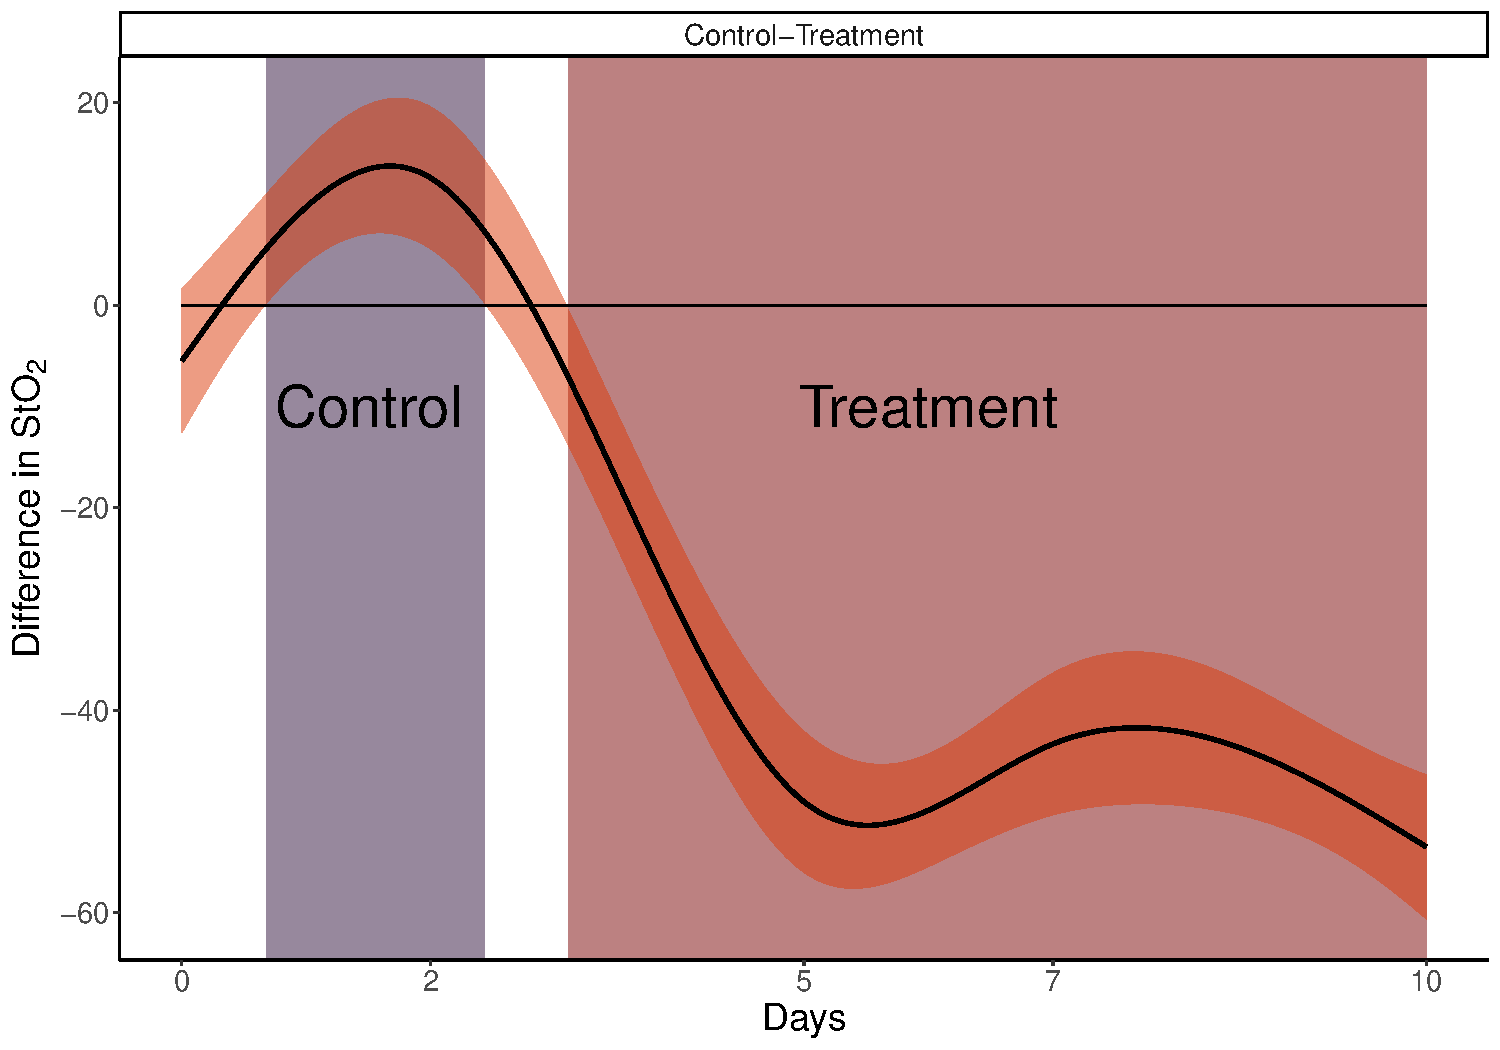
\includegraphics[width=0.75\linewidth,]{00-Full_document_files/figure-latex/pairwise-comp-workflow-fig-1} 

}

\caption{Smooth pairwise comparisons for model \passthrough{\lstinline!m1!} using a 95\% confidence interval for the difference between smooths. The comparison is centered at the response scale. Shaded regions indicate time intervals where each treatment group has a non-zero effect.}\label{fig:pairwise-comp-workflow-fig}
\end{figure}

Of notice, a convenient wrapper for the function described above exists in the package \passthrough{\lstinline!gratia!}. In this package, \passthrough{\lstinline!difference\_smooths!} is a function that makes the comparisons and produces Figure \ref{fig:pairwise-comp-workflow-fig} when is used on a fitted model. The function syntax and an example can be found at:

\url{https://cran.r-project.org/web/packages/gratia/gratia.pdf}

Keep in mind that this function \textbf{does not} center the pairwise comparison at the response scale, so it has to be shifted in order to be compared to the raw data.

\hypertarget{gam-and-linear-model-plots-and-missing-data}{%
\section{GAM and Linear model plots and Missing data}\label{gam-and-linear-model-plots-and-missing-data}}

This section covers the code used to generate Figure \ref{fig:sim-smooth-plot}, where the simulated data, fit of the ``final'' GAM (\passthrough{\lstinline!m1!}), linear model and GAM on data with missing observations are presented. Note that panel A in Figure \ref{fig:sim-smooth-plot} and the inset are generated in the code chunk where the data is simulated in Section \ref{tumor-data-simulation}, and are called later to build the figure.

\hypertarget{gam-and-linear-model-plots}{%
\subsection{GAM and Linear model plots}\label{gam-and-linear-model-plots}}

This code chunk creates panels B and D in Figure \ref{fig:sim-smooth-plot}. Note that this code uses the final GAM from the previous section (\passthrough{\lstinline!m1!}), so the simulated data and the model should be generated before running this section.

\begin{lstlisting}[language=R]
#linear model
lm1<-lm(StO2_sim ~ Day + Group + Day * Group, data = dat_sim)


#creates a dataframe using the length of the covariates for the GAM
gam_predict <- expand_grid(Group = factor(c("Control", "Treatment")),
                         Day = seq(0, 10, by = 0.1),
                         subject=factor(rep(1:10)))

#creates a dataframe using the length of the covariates for rm-ANOVA
lm_predict<-expand_grid(Group = factor(c("Control", "Treatment")),
                         Day = c(0:10),
                        subject=factor(rep(1:10)),
                          )
lm_predict$subject<-factor(paste(lm_predict$subject, lm_predict$Group, sep = "-"))

#adds the predictions to the grid and creates a confidence interval for GAM
gam_predict<-gam_predict%>%
    mutate(fit = predict(m1,gam_predict,se.fit = TRUE,type='response')$fit,
           se.fit = predict(m1, gam_predict,se.fit = TRUE,type='response')$se.fit)

#using lm
lm_predict<-lm_predict%>%
    mutate(fit = predict(lm1,lm_predict,se.fit = TRUE,type='response')$fit,
           se.fit = predict(lm1, lm_predict,se.fit = TRUE,type='response')$se.fit)

#plot smooths and confidence interval for GAM
f3<-ggplot(data=dat_sim, aes(x=Day, y=StO2_sim, group=Group)) +
    geom_point(aes(color=Group),size=1.5,alpha=0.5,show.legend = FALSE)+
  geom_ribbon(aes( x=Day,ymin=(fit - 2*se.fit), 
                   ymax=(fit + 2*se.fit),
                   fill=Group
                   ),
              alpha=0.3,
              data=gam_predict,
            show.legend=FALSE,
                inherit.aes=FALSE) +
  geom_line(aes(y=fit,
                color=Group),
              size=1,data=gam_predict,
              show.legend = FALSE)+
  #facet_wrap(~Group)+
  labs(y=expression(atop(StO[2],'complete')))+
    scale_x_continuous(breaks=c(0,2,5,7,10))+
      theme_classic()+
  theme(
    axis.text=element_text(size=22)
  )+
      thm+
  thm1
 
#plot linear fit for rm-ANOVA
f4<-ggplot(data=dat_sim, aes(x=Day, y=StO2_sim, group=Group)) +
    geom_point(aes(color=Group),size=1.5,alpha=0.5,show.legend = FALSE)+
  geom_ribbon(aes( x=Day,ymin=(fit - 2*se.fit), 
                   ymax=(fit + 2*se.fit),fill=Group),
              alpha=0.3,
              data=lm_predict,
              show.legend = FALSE,
                inherit.aes=FALSE) +
  geom_line(aes(y=fit,
                color=Group),
              size=1,data=lm_predict,
              show.legend = FALSE)+
  #facet_wrap(~Group)+
  labs(y=expression(paste('StO'[2],' (simulated)')))+
    scale_x_continuous(breaks=c(0,2,5,7,10))+
      theme_classic()+
  theme(
    axis.text=element_text(size=22)
  )+
      thm+
  thm1
 


#posthoc comparisons for the linear model
#library(multcomp)


#summary(glht(lm1, linfct = mcp(Group = 'Tukey')))
#summary(glht(lm1, linfct=mcp(Group="Tukey", interaction_average=TRUE)))
\end{lstlisting}

\hypertarget{working-with-missing-data-in-gams}{%
\subsection{Working with Missing data in GAMs}\label{working-with-missing-data-in-gams}}

This code chunk first randomly deletes 40\% of the total observations in the original simulated data, and then an interaction GAM is fitted to the remaining data. Model diagnostics are presented, and an object that stores the fitted smooths is saved to be called in the final code chunk to build the figure.

\begin{lstlisting}[language=R]
#missing data
#create a sequence of 40 random numbers between 1 and 100, these numbers will
#correspond to the row numbers to be randomly erased from the original dataset

missing <- sample(1:100, 40)

#create a new dataframe from the simulated data with 40 rows randomly removed, keep the missing values as NA

ind <- which(dat_sim$StO2_sim %in% sample(dat_sim$StO2_sim, 40))

#create a new dataframe, remove the StO2 column
dat_missing <- dat_sim[,-1]

#add NAs at the ind positions
dat_missing$StO2_sim[ind]<-NA 

#Count the number of remaining observations per day (original dataset had 10 per group per day)
dat_missing %>%
    group_by(Day,Group) %>%
    filter(!is.na(StO2_sim))%>%
  count(Day)


#the same model used for the full dataset
mod_m1 <- gam(StO2_sim ~ Group+s(Day,by=Group,k=5), data  = dat_missing,family=scat)
#appraise the model
appraise(mod_m1)


m_predict <- expand_grid(Group = factor(c("Control", "Treatment")),
                         Day = seq(0, 10, by = 0.1))

#adds the predictions to the grid and creates a confidence interval
m_predict<-m_predict%>%
    mutate(fit = predict(mod_m1,m_predict,se.fit = TRUE,type='response')$fit,
           se.fit = predict(mod_m1, m_predict,se.fit = TRUE,type='response')$se.fit)


f6<-ggplot(data=dat_missing, aes(x=Day, y=StO2_sim, group=Group)) +
    geom_point(aes(color=Group),size=1.5,alpha=0.5,show.legend = FALSE)+
  geom_ribbon(aes( x=Day,ymin=(fit - 2*se.fit), 
                   ymax=(fit + 2*se.fit),
                   fill=Group
                   ),
              alpha=0.3,
              data=m_predict,
            show.legend=FALSE,
                inherit.aes=FALSE) +
  geom_line(aes(y=fit,
                color=Group),
              size=1,data=m_predict,
              show.legend = TRUE)+
  #facet_wrap(~Group)+
  labs(y=expression(atop(StO[2],'missing')))+
    scale_x_continuous(breaks=c(0,2,5,7,10))+
      theme_classic()+
  theme(
    axis.text=element_text(size=22)
  )+
      thm+
  thm1
\end{lstlisting}

\begin{figure}[H]

{\centering 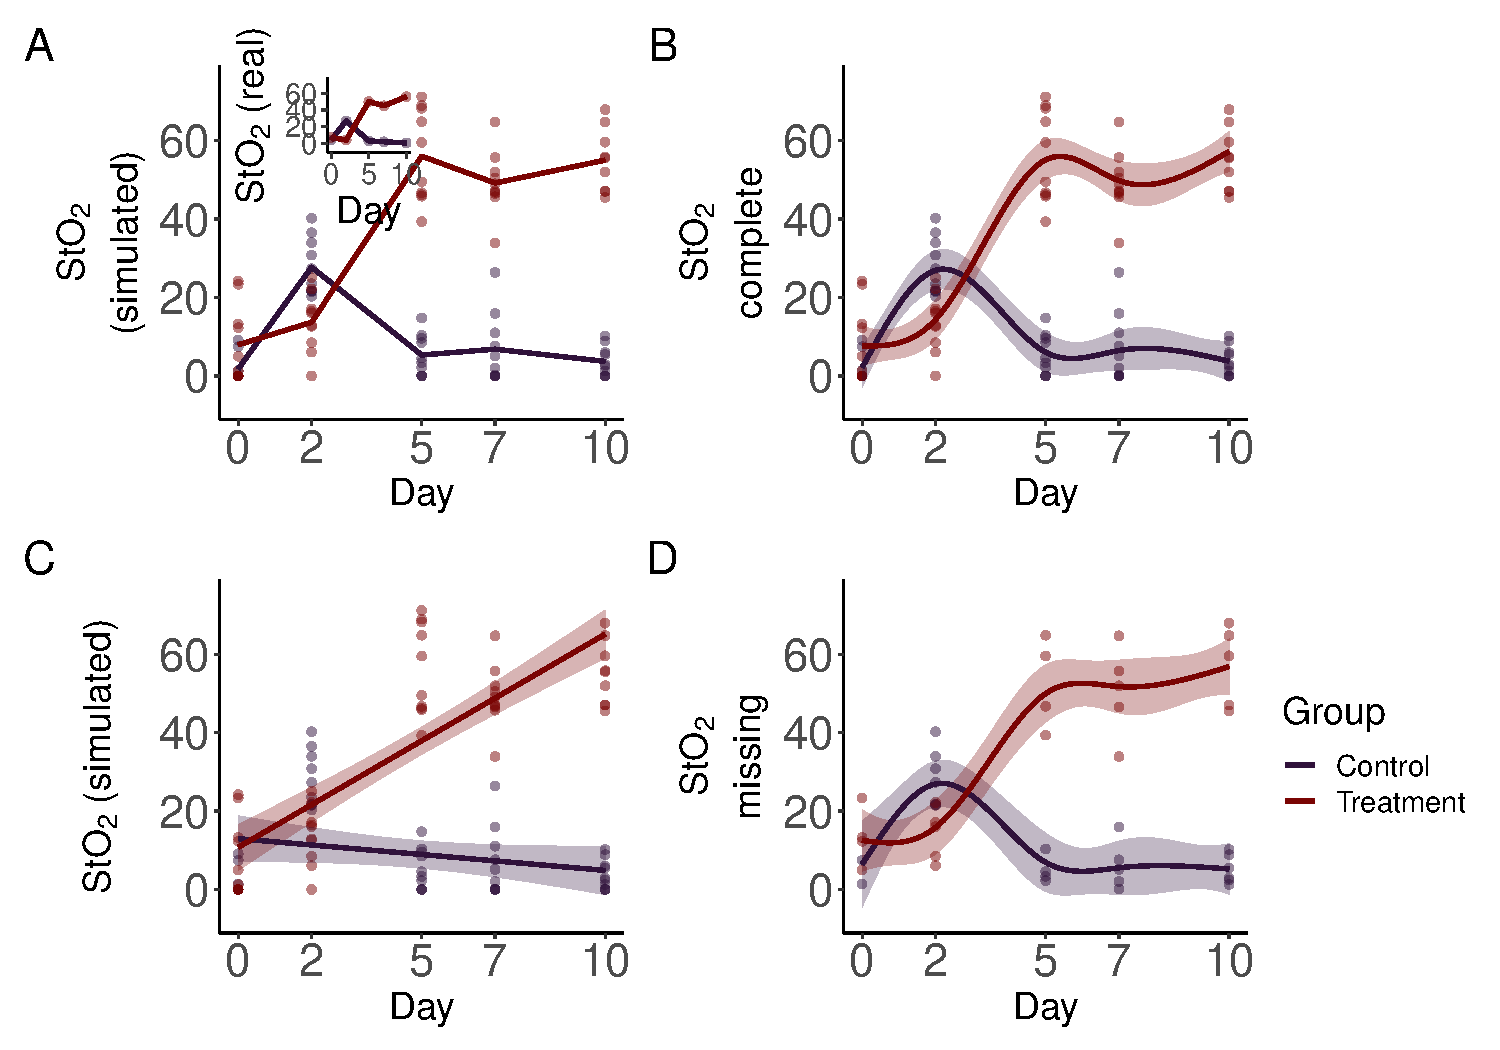
\includegraphics[width=0.75\linewidth,]{00-Full_document_files/figure-latex/sim-smooth-plot-Appendix-1} 

}

\caption{Simulated data and smooths for oxygen saturation in tumors. A: Simulated data that follows previously reported trends (inset) in tumors under chemotherapy (Treatment) or saline (Control) treatment. Simulated data is from a normal distribution with standard deviation of 10\% with 10 observations per time point. Lines indicate mean oxygen saturation B: Smooths from the GAM model for the full simulated data with interaction of Group and Treatment. Lines represent trends for each group, shaded regions are 95\% confidence intervals. C: The rm-ANOVA model for the simulated data, which does not capture the changes in each group over time. D: Smooths for the GAM model for the simulated data with 40\% of its observations missing. Lines represent trends for each group, shaded regions are 95\% empirical Bayesian confidence intervals.}\label{fig:sim-smooth-plot-Appendix}
\end{figure}

\hypertarget{pairwise-comparisons-in-gams-full-and-missing-data-cases}{%
\subsection{Pairwise comparisons in GAMs: full and missing data cases}\label{pairwise-comparisons-in-gams-full-and-missing-data-cases}}

The next code chunk reproduces Figure \ref{fig:plot-pairwise-comp}. Here pairwise comparisons are made for the full and missing datasets.

\begin{lstlisting}[language=R]
##Pairwise comparisons

pdat <- expand.grid(Day = seq(0, 10, length = 400),
                    Group = c('Control', 'Treatment'))

#this function takes the model, grid and groups to be compared using the lpmatrix
#originally developed by G. Simpson:
#https://fromthebottomoftheheap.net/2017/10/10/difference-splines-i/

smooth_diff <- function(model, newdata, g1, g2, alpha = 0.05,
                        unconditional = FALSE) {
    xp <- predict(model, newdata = newdata, type = 'lpmatrix')
    #Find columns in xp where the name contains "Control" and "Treatment"
    col1 <- grepl(g1, colnames(xp))
    col2 <- grepl(g2, colnames(xp))
    #Find rows in xp that correspond to each treatment
    row1 <- with(newdata, Group == g1)
    row2 <- with(newdata, Group == g2)
    ## difference rows of xp for data from comparison
    X <- xp[row1, ] - xp[row2, ]
    ## zero out cols of X related to splines for other lochs
    X[, ! (col1 | col2)] <- 0
    
    ## zero out the parametric cols
    #This line has been commented to keep the comparison at the response level,
    #otherwise it gives the marginal change between smooths
    #X[, !grepl('^s\\(', colnames(xp))] <- 0
    dif <- X %*% coef(model)
    #get standard error, critical value and boundaries
    se <- sqrt(rowSums((X %*% vcov(model, unconditional = unconditional)) * X))
    crit <- qt(alpha/2, df.residual(model), lower.tail = FALSE)
    upr <- dif + (crit * se)
    lwr <- dif - (crit * se)
    data.frame(pair = paste(g1, g2, sep = '-'),
               diff = dif,
               se = se,
               upper = upr,
               lower = lwr)
}

#use the function to calculate the difference in smooths
comp1<-smooth_diff(m1,pdat,'Control','Treatment')

#Create a dataframe with time, comparisons and labels for regions where difference exists
comp_StO2_full <- cbind(Day = seq(0, 10, length = 400),
                   rbind(comp1)) %>%
  mutate(interval=case_when(
    upper>0 & lower<0~"no-diff",
    upper<0~"less",
    lower>0~"greater"
  ))

pairwise_limits<-function(dataframe){
    #extract values where the lower limit of the ribbon is greater than zero
    #this is the region where the control group effect is greater
    v1<-dataframe%>%
        filter(lower>0)%>%
        select(Day)
    #get day  initial value
    init1=v1$Day[[1]]
    #get day final value
    final1=v1$Day[[nrow(v1)]]

    #extract values where the value of the upper limit of the ribbon is lower than zero
    #this corresponds to the region where the treatment group effect is greater
    v2<-comp_StO2_full%>%
        filter(upper<0)%>%
        select(Day)

    init2=v2$Day[[1]]
    final2=v2$Day[[nrow(v2)]]
    #store values
    my_list<-list(init1=init1,
                  final1=final1,
                  init2=init2,
                  final2=final2)
return(my_list)
}

my_list<-pairwise_limits(comp_StO2_full)
rib_col<-'#EDD03AFF'

c1<-ggplot(comp_StO2_full, aes(x = Day, y = diff, group = pair)) +
    annotate("rect",
                xmin =my_list$init1, xmax =my_list$final1,ymin=-Inf,ymax=Inf,
                fill='#30123BFF',
                alpha = 0.5,
                ) +
  annotate("text",
             x=1.5,
             y=-18,
             label="Control>Treatment",
           size=8,
           angle=90
           )+
    annotate("rect",
             xmin =my_list$init2, xmax =my_list$final2,ymin=-Inf,ymax=Inf,
             fill='#7A0403FF',
             alpha = 0.5,
    ) +
  annotate("text",
             x=6,
             y=-18,
             label="Treatment>Control",
             size=8,
           angle=90
           )+
    geom_ribbon(aes(ymin = lower, ymax = upper),
                alpha = 0.5,
                fill=rib_col) +
    geom_line(data=comp_StO2_full,aes(y=0),size=0.5)+
    geom_line(color='black',size=1) +

    facet_wrap(~ pair) +
    theme_classic()+
    labs(x = 'Days', y = expression(paste('Difference in StO'[2] )))+
    scale_x_continuous(breaks=c(0,2,5,7,10))+
    theme(
        text=element_text(size=18),
        legend.title=element_blank()
    )


###for missing data
comp2<-smooth_diff(mod_m1,pdat,'Control','Treatment')
comp_StO2_missing <- cbind(Day = seq(0, 10, length = 400),
                   rbind(comp2))

missing_plot<-ggplot(comp_StO2_missing, aes(x = Day, y = diff, group = pair)) +
    geom_ribbon(aes(ymin = lower, ymax = upper), alpha = 0.2) +
    geom_line(color='black',size=1) +
    facet_wrap(~ pair) +
    labs(x = 'Days', 
         y = expression(paste('Difference in StO'[2],'\n (missing data)' 
                              )))+
  scale_x_continuous(breaks=c(0,2,5,7,10))+
  theme_classic()+
  theme(
     text=element_text(size=18),
     legend.title=element_blank()
     )

my_list<-pairwise_limits(comp_StO2_missing)

c2<-ggplot(comp_StO2_missing, aes(x = Day, y = diff, group = pair)) +
    annotate("rect",
             xmin =my_list$init1, xmax =my_list$final1,ymin=-Inf,ymax=Inf,
             fill='#30123BFF',
             alpha = 0.5,
    ) +
  annotate("text",
             x=1.5,
             y=-18,
             label="Control>Treatment",
           size=8
           )+
    annotate("rect",
             xmin =my_list$init2, xmax =my_list$final2,ymin=-Inf,ymax=Inf,
             fill='#7A0403FF',
             alpha = 0.5,
    ) +
  annotate("text",
             x=6,
             y=-18,
             label="Treatment>Control",
             size=8)+
    geom_ribbon(aes(ymin = lower, ymax = upper),
                alpha = 0.5,
                fill=rib_col) +
    geom_line(data=comp_StO2_missing,aes(y=0),size=0.5)+
    geom_line(color='black',size=1) +
    facet_wrap(~ pair) +
    theme_classic()+
    labs(x = 'Days', y = expression(paste('Difference in StO'[2] )))+
    scale_x_continuous(breaks=c(0,2,5,7,10))+
    theme(
        text=element_text(size=18),
        legend.title=element_blank()
    )

pair_comp<-c1+c2
\end{lstlisting}

\begin{figure}[H]

{\centering 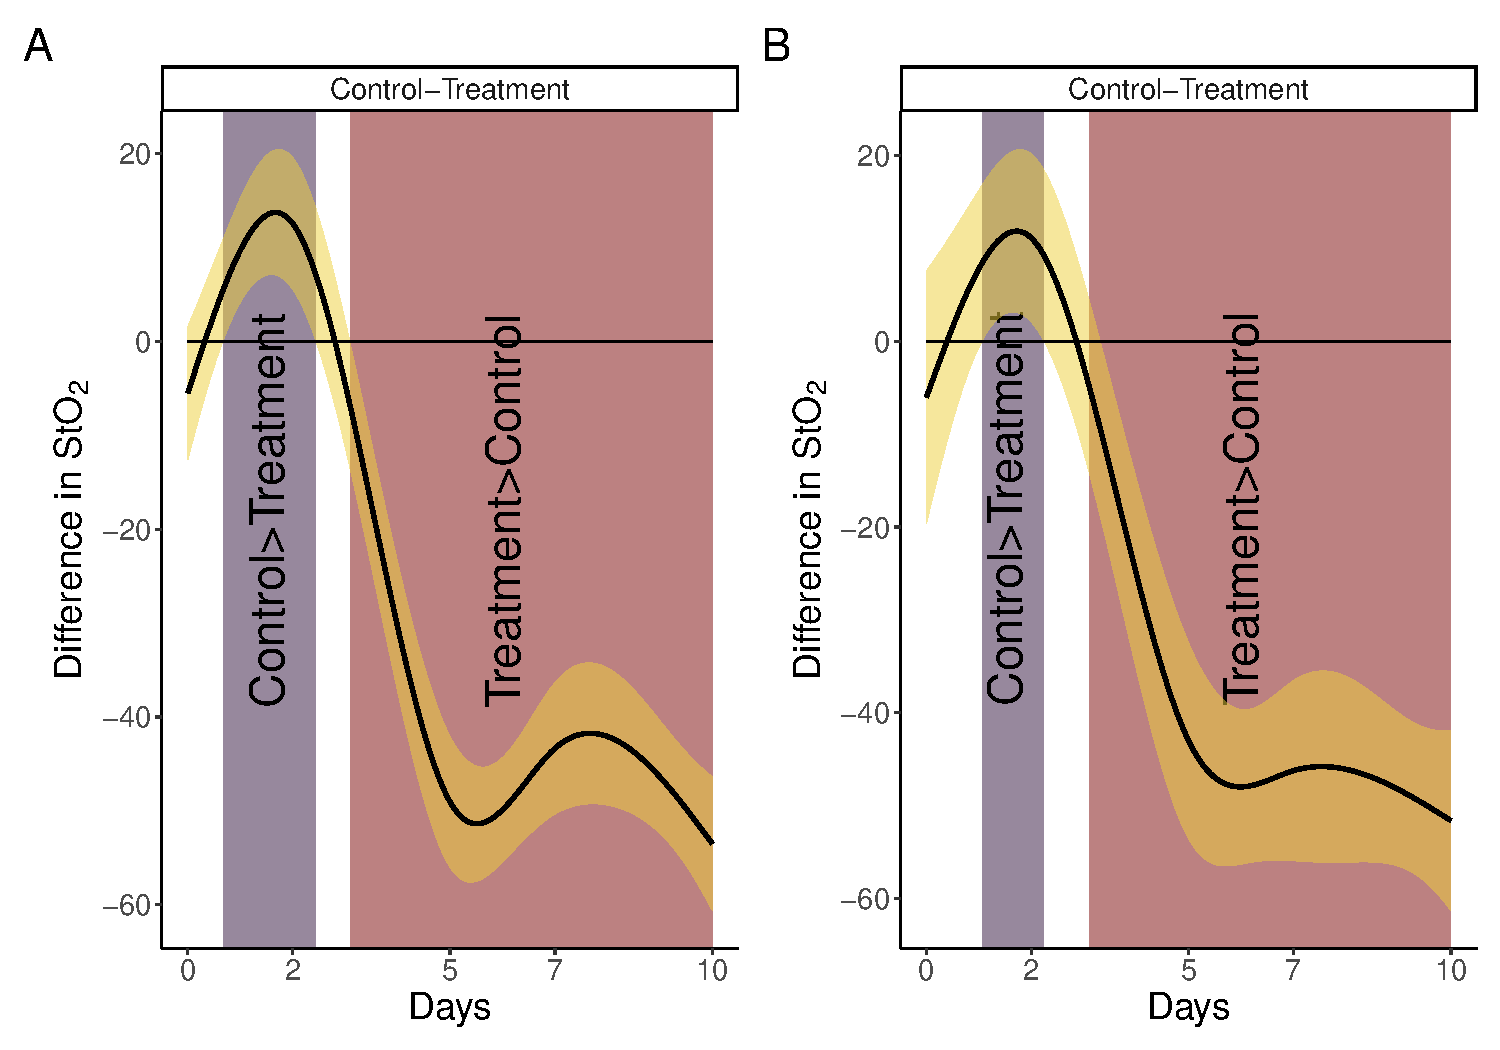
\includegraphics[width=0.75\linewidth,]{00-Full_document_files/figure-latex/plot-pairwise-comp-Appendix-1} 

}

\caption{Pairwise comparisons for smooth terms. A: Pairwise comparisons for the full dataset. B: Pairwise comparisons for the dataset with missing observations. Significant differences exist where the 95\% empirical Bayesian credible interval does not cover 0. In both cases the effect of treatment is significant after day 3.}\label{fig:plot-pairwise-comp-Appendix}
\end{figure}

\end{document}
